\documentclass[tikz,12pt,margin=0px]{article}

\usepackage[a4paper,bindingoffset=0.2in,
            left=1.5cm,right=1.5cm,top=1.25cm,bottom=1.5cm,%
            footskip=.25in]{geometry}
\usepackage[normalem]{ulem}
\usepackage[utf8]{inputenc}
\usepackage{amsmath}
\usepackage{amssymb}
\usepackage{comment}
\usepackage{enumitem}
\usepackage{fancyhdr}
\usepackage{float}
\usepackage{fontawesome}
\usepackage{makecell}
\usepackage{tikz}
\usepackage{titlesec}
\usepackage[hungarian]{babel}
\usetikzlibrary{positioning,calc,shapes.multipart,arrows,arrows.meta,matrix,automata,shapes.misc}

\setlist[itemize,1]{label=$\bullet$}
\setlist[itemize,2]{label=$\circ$}
\setlist[itemize,3]{label=$\centerdot$}
\setlist[itemize,4]{label=$\cdot$}

\titleformat*{\section}{\Large\bfseries}
\titleformat*{\subsection}{\large\bfseries}
\titleformat*{\subsubsection}{\normalsize\bfseries}
\titleformat*{\paragraph}{\small\bfseries}
\titleformat*{\subparagraph}{\footnotesize\bfseries}

\pagestyle{fancy}

\newcommand\blfootnote[1]{%
  \begingroup
  \renewcommand\thefootnote{}\footnote{#1}%
  \addtocounter{footnote}{-1}%
  \endgroup
}

\renewcommand{\figurename}{ábra}

\makeatletter
\renewcommand\paragraph{%
	\@startsection{paragraph}{4}{0mm}%
	{-\baselineskip}%
	{.5\baselineskip}%
	{\normalfont\normalsize\bfseries}}
\makeatother

\useunder{\uline}{\ul}{}
\fancyhead{}
\cfoot{15. tétel | \thepage. oldal}

\renewcommand{\headrulewidth}{0pt}
\renewcommand{\footrulewidth}{0.4pt}

{\par
\hyphenpenalty=10000
\exhyphenpenalty=10000
}
{\par}

\newcommand\lword[1]{\leavevmode\nobreak\hskip0pt plus\linewidth\penalty50\hskip0pt plus-\linewidth\nobreak #1}

\begin{document}

    \thispagestyle{fancy}
    \hyphenation{oddword}
    \uchyph=0

    \begin{center}
        {\Large\bfseries\noindent 15. Operációs rendszerek} \\
    \end{center}

	\section*{Folyamatok megvalósítása, ütemező algoritmusaik}
	
    \subsection*{Folyamatok}

    A \emph{program} egy bájthalmaz a fájlrendszerben. A \emph{folyamat} egy futó program példánya a memóriában: kód + I/O adatok + állapot. Annyiszor jön létre, ahányszor a programot elindítjuk.\\

    \noindent Egy folyamat élettartamának vezérlése az operációs rendszer feladata:

    \begin{enumerate}[topsep=8pt,itemsep=4pt,partopsep=4pt, parsep=4pt]
        \item létrehozás
        \item ütemezés (folyamatok közti váltás)
        \item megszüntetés
    \end{enumerate}

    \paragraph*{Folyamatok létrehozása}

    A működésre kész operációs rendszerben például interaktív kiszolgálás esetén minden terminálhoz tartozhat egy rendszerfolyamat, amelyik felhasználói parancsokat fogad és hajt végre. Kötegelt feldolgozás esetén elindulhat egy jobkészletet kezelő folyamat, amelyik jobok végrehajtását kezdi meg és jobonként egy újabb folyamatot indít. Valós idejű rendszer esetén az operációs rendszer saját felépülése után létrehozza és inicializálja a felhasználói rendszert alkotó folyamatokat.\\

    \noindent A rendszerfolyamatok tehát újabb, felhasználói folyamatokat hoznak létre, a felhasználói folyamatok pedig – bizonyos típusú rendszerekben – maguk is létrehozhatnak további felhasználói folyamatokat a logikai processzor megfelelő utasításának végrehajtásával (például fork, create).\\

	\paragraph*{Folyamatok befejezése}

    Egy folyamat az elindulása után a megadott időkeretben (el)végzi a feladatát. A befejezés lehet önkéntes vagy önkéntelen.
	\begin{itemize}[topsep=8pt,itemsep=4pt,partopsep=4pt, parsep=4pt]
        \item Önkéntes befejezések:
        \begin{itemize}
            \item szabályos kilépés (exit, return stb.)
            \item kilépés lekezelt hiba esetén (szintén pl. return utasítással)
        \end{itemize}
        \item Önkéntelen befejezések:
        \begin{itemize}
            \item illegális utasítás
            \item végzetes hiba (0-val osztás, nem létező memória használat, stb)
            \item egy másik folyamat által
            \item felhasználói megszakítás
        \end{itemize}
	\end{itemize}

    \noindent A folyamatok futhatnak előtérben, illetve a háttérben (démonok).\\

    \noindent Azokat a rendszereket, amelyek működése során – a felépülés és inicializálás kezdeti szakaszától eltekintve – nem jönnek létre és nem szűnnek meg folyamatok, \emph{statikus rendszereknek} nevezzük, szemben a \emph{dinamikus rendszerekkel}, amelyekben működés közben bármikor születhetnek és \lword{megszűnhetnek} a folyamatok.\\

    \noindent A folyamatok eredetét szükség esetén a szülő–gyermek viszonyokkal, azaz egy fa struktúrával írhatjuk le (processzgráf). Dinamikus rendszerben a fa természetesen folyamatosan követi a folyamatok születését és halálát. Sok operációs rendszer a szülő–gyermek viszonyokra építi erőforrás-gazdálkodási és jogosultsági filozófiáját. Ennek egyik megközelítése a hierarchikus erőforrás-gazdálkodás, amikor a gyermek folyamatok csak a szülő erőforrásaiból részesülhetnek és nem létezhetnek önállóan, csak amíg szülőjük is létezik. Egy másik megközelítés a globális erőforrás-gazdálkodás, amikor a rendszer valamennyi folyamata létrejötte után egyenrangú, önálló szereplő, és versenyezhet a teljes erőforráskészletből való részesedésért.

    \subsection*{Folyamatállapotok}

    \noindent A mai modern számítógép fogalmához hozzátartozik, hogy természetesnek vesszük azt, amikor a számítógépünk egyidejűleg több tevékenységet végez. Például zenehallgatás közben böngészünk a neten.\\

    \noindent Hogyan lehetséges ez, ha a számítógépünkben egy processzor (CPU) van, és az egyidejűleg csak egy feladatot képes végrehajtani?\\

    \noindent Erre a kérdésre a válasz a végrehajtás sebességében van. A központi egység olyan gyorsan képes végrehajtani az utasításokat (több millió utasítást másodpercenként), hogy ha ennél a sebességnél váltogatjuk az éppen végrehajtódó feladatokat, az számunkra azt az illúziót kelti, mintha egymással párhuzamosan történnének a feladat-végrehajtások (ál-multitasking).\\

    \noindent A folyamatok közti gyors kapcsolást, a végrehajtás váltását \emph{multiprogramozás}nak nevezzük.\\

\begin{comment}
    {\footnotesize \noindent {\color{blue} \faLightbulbO\ $\triangleright$ } }
    {\footnotesize
    \noindent A mai számítógép egyrészt nem egy processzort, hanem több, önálló végrehajtási egységet foglal magában, másrészt egy fizikai processzor ráadásul több (kettő, négy vagy akár nyolc) magot is tartalmazhat.\\

    \noindent A központi egységekben minden magnak saját belső memóriája van, ahova a közös fizikai memóriából betöltik az éppen végrehajtandó feladat kódját, és ekkor a magok valódi párhuzamos működést mutatnak. Ez azt jelenti, hogy egy időegység alatt (körülbelül egy óraciklus) mindegyik mag végrehajtja a saját folyamatának utasítását.\\

    \noindent Ekkor nem látszatpárhuzamosságról beszélhetünk, de ez nem befolyásolja érdemben azt, hogy a folyamatok fogalmi modelljén (szekvenciális, egymás után végrehajtódó folyamatok sora) módosítsunk, amelynek segítségével a párhuzamosság\footnote{Programok vagy programfolyamatok egy idejű, egymás melletti futása} kezelését tudjuk végezni.\\

    \noindent Így ebben az értelemben a számítógépen futó „program” – magával az operációs rendszer feladataival együtt – nem más, mint szekvenciális folyamatok sorozata. A folyamat egy végrehajtás alatt álló program, és ehhez a folyamathoz tartoznak természetesen más jellemzők is még, mint például a központi egység utasításszámlálója (hol tart a folyamatban a végrehajtás), a központi egység regiszterei (a végrehajtási számítások segédértékei) és a folyamat egyéb más állapotleírói. Ahhoz, hogy egyik folyamatról a másikra tudjunk váltani, az szükséges, hogy mindezen leírókat, adatokat mentsük, hiszen ezek ismerete feltétlenül szükséges a folyamat egy későbbi időpillanatban történő folytatásához.
    $\triangleleft$ \faLightbulbO}\\
\end{comment}
    \noindent A folyamatok önálló egységek, a memória egy kis szeletében helyezkednek el. Ahhoz, hogy a központi egység ezeket végre tudja hajtani, a folyamatokhoz tartozzon saját utasításszámláló, verem, és legyenek egyéb állapotjelzői.\\

    \noindent A folyamatok közül biztosan egy folyamat fut mindig, és az összes többi arra vár, hogy lehetőséget kapjon a futásra.\\

    \noindent A folyamatok gyakran nemcsak önmagukban számolnak, végeznek feladatokat, hanem az operációs rendszer lehetőségeit is igénybe vehetjük: rendszerhívás\footnote{A rendszerhívás olyan speciális eljáráshívás, amikor a hívások egy kritikus feladat végrehajtására a kernelbe vagy más privilegizált operációs rendszerbeli komponensbe irányulnak. Ilyen rendszerhívások például egy állomány írására, olvasására, átnevezésére irányuló programhívásoké.} formájában kérhetünk segítséget ahhoz, hogy egy program vagy az operációs rendszer fennhatósága alá eső fájlokkal (eszközzel) vagy egy másik folyamattal kommunikáljunk. A folyamatok működése során gyakori feladat, hogy más alkalmazás szolgáltatását vegyük igénybe.\\

    \noindent A várakozó folyamatokat több csoportba sorolhatjuk az operációs rendszerektől függően. Bármilyen csoportosítást is nézünk, jellemzően két lényeges csoport különböztethető meg a várakozó folyamatok között.\\

    \noindent Ebből talán a folyamatok többségét a \textbf{futásra készen álló folyamatok} adják, melyeknek nincs semmire szükségük, csak arra, hogy újra „processzorhoz jussanak”! A másik csoportot a \textbf{blokkolt folyamatok} alkotják, melyeknek további működéséhez szükségük van egy másik folyamat eredményére vagy valamilyen adatára. Ezek nem tudnak futni még akkor sem, ha processzoridőt kapnának.\\
\newpage
    \noindent A csoportok között az alábbi négy átmenetet különböztethetjük meg:

    \begin{itemize}[topsep=8pt,itemsep=4pt,partopsep=4pt, parsep=4pt]
        \item Futó $\rightarrow$ Blokkolt
            \begin{itemize}
                \item Várni kell még valamire. A futó folyamat nem tudja folytatni a futását, mert valamilyen bemeneti adatra van szüksége. Ez akár egy másik folyamat eredménye is lehet.
            \end{itemize}
        \item Futó $\rightarrow$ Futásra kész
            \begin{itemize}
                \item Ez egy természetes átmenet. Egyszerűen lejárt az aktuális folyamat processzorideje, és az operációs rendszer a folyamatot a futásra kész, várakozó folyamatok csoportjába sorolja.
            \end{itemize}
        \item Futásra kész $\rightarrow$ Futó
            \begin{itemize}
                \item Az előző átmenet fordítottja. Az operációs rendszer ütemezője a futásra készen várakozó folyamatok csoportjából a soron következő folyamatot futtatja. A sorrendről az ütemező dönt, a folyamatok nem nagyon tudnak róla, hogy melyikük fog következni.
            \end{itemize}
        \item Blokkolt $\rightarrow$ Futásra kész
            \begin{itemize}
                \item A várva várt adat megérkezett, a blokkolt folyamat marad még a várakozó folyamatok csoportjában, de már futásra készen várja, hogy az ütemező döntése esetén újra futhasson.
            \end{itemize}
    \end{itemize}

    \noindent A folyamatok négy állapotátmenetét és a hozzájuk tartozó három állapotot szemléletesebb formában az \ref{allapotatmentek}. ábra mutatja.

	\begin{figure}[H]
		\centering
		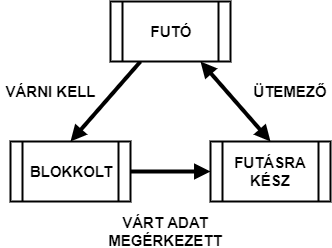
\includegraphics[width=0.5\textwidth]{img/allapot.png}
		\caption{Állapotátmenetek}
        \label{allapotatmentek}
	\end{figure}

    \noindent \textit{További állapotok}: alvó, megállított, és zombi. A zombi állapotban ha egy gyermek folyamat befejeződik, de szülője nem hív wait(\&st) hívást, akkor a gyermek bent marad a processztáblában, init folyamat törli ezeket.\\

    \noindent Egy processzoron egyszerre egy futó folyamat lehet. Üres processzoron az \emph{Idle} folyamat fut, ami nem csinál semmit.\\
	
    \noindent Az operációs rendszernek ahhoz, hogy ezeket a folyamatokat helyesen tudja kezelni, felügyelnie kell a folyamatokat. Az operációs rendszerünk így minden egyes folyamatot nyilvántart, és az operációs rendszer lelkének is nevezett ütemező (scheduler) segítségével szépen sorban minden egyes folyamatnak ad egy kis processzor- (CPU) időszeletet, amíg az adott folyamat dolgozik, azaz a processzorra kerülhet.

    \paragraph*{Folyamatok leírása és táblázata}

    \noindent Ahhoz, hogy a folyamatokat megfelelően tudja ütemezni az operációs rendszer, nyilván kell tartani minden olyan információt, ami a folyamat újraütemezéséhez szükséges. A nyilvántartáshoz az operációs rendszer egy táblázatot használ, amit \textbf{folyamattáblázatnak} vagy \textbf{folyamatvezérlő blokknak} (Process Control Block – PCB) neveznek.\\

    \noindent Ebben a táblázatban minden olyan információ tárolva kell legyen, ami ahhoz kell, hogy a folyamatot a futó állapotából a futásra kész állapotba hozzuk át, majd ha újra futó állapotba kerül, akkor úgy folytathassa a futását, mintha semmi sem történt volna.\\

    \noindent A teljesség igénye nélkül egy folyamathoz tartozó ilyen adatok:
    \begin{itemize}[topsep=8pt,itemsep=4pt,partopsep=4pt, parsep=4pt]
        \item a folyamat utasításszámlálója,
        \item a folyamat veremmutatója,
        \item a processzor regisztereinek adatai,
        \item a nyitott fájlok állapotinformációja,
        \item a memória (kapcsolódó) adatai,
        \item stb.
    \end{itemize}

\begin{comment}
    {\footnotesize \noindent {\color{blue} \faLightbulbO\ $\triangleright$ } }
    {\footnotesize
    \noindent Ez az adatmennyiség nem is olyan kevés, nagyon fontos a mentési és a visszaolvasási hatékonyság. Ha sok időt igényel, akkor az azzal jár, hogy az operációs rendszer ütemezője leköti a rendszererőforrások nagy részét. Bár ezen segít a processzorok egyre nagyobb teljesítménye, de nem lenne elég, ha nem társulna hozzá processzortámogatás. Az x486 processzorcsalád megjelenése óta a folyamatállapot szegmens (Task State Segment – TSS\footnote{Task State Segment, más néven folyamatállapot szegmens. Feladata a folyamatokkal kapcsolatos információk tárolása pl. azonosító, folyamat állapota stb.}, minden folyamatnak van ilyen) segítségével gyorsítja a váltást, illetve a folyamatregiszter (Task Register – TR) tartalmazza az aktív folyamat TSS leíróját. Ennek a cseréje gyors (általában egy-két gépi óraciklus), így ezek révén a folyamatok váltása nagyon hatékony.\\

    \noindent A folyamattábla legfontosabb mezői (teljesség igénye nélkül):

    \begin{itemize}
        \item Kernel információk:
        \begin{itemize}
            \item a regiszterek, az utasításszámláló, a folyamatállapot, a veremmutató, az aktuális ütemezési prioritás, a maximális ütemezési prioritás, az időzítési egység mérete, a felhasznált processzoridő (CPU idő) stb.
        \end{itemize}
        \item Folyamatkezelő információk:
        \begin{itemize}
            \item a kódszegmens-mutató, az adatszegmens-mutató, a szignálállapot, a kilépési állapot, a folyamat azonosítója (PID), a szülőfolyamat azonosítója (PPID), a gyermekfolyamatok processzorideje, a valódi felhasználói azonosító (UID), a valódi csoportazonosító (GID), a folyamat neve stb.
            \end{itemize}
        \item Fájlkezelő információk:
        \begin{itemize}
            \item az umask-érték (user mask), a gyökérkönyvtár, a munkakönyvtár, a fájlleírók, a valós felhasználói azonosító (UID), a valós csoportazonosító (GID), a TTY vezérlő stb.
        \end{itemize}
    \end{itemize}

    \noindent A hardvereszközök kezelésének alapja minden mai operációs rendszerben a megszakításelven működik. Adott egy táblázat, aminek sorszáma a megszakítás\footnote{Egy olyan (általában külső) esemény, amelynek hatására a program futása félbemarad. A megszakításokat egy szám (1 bájt méretű) azonosítja, az int utasításnak is ez a paramétere. A megszakítás azonosító száma alapján a processzor meg tudja állapítani, hogy milyen esemény történt.} számát jelenti, míg a táblázat eleme megadja a kiszolgálórutin címét. Ezt a táblát megszakításvektornak nevezzük. Ilyen kiszolgálási elvre épül az ütemező időzítője is. Ekkor az ütemező, az időzítő kiszolgálórutinja az aktuális folyamatot lecseréli a következőre.\\

    \noindent Tegyük fel, hogy egy folyamat adatot vár egy lemezegységtől. Az adat hozzáférhetőségét a lemezegység egy megszakításkéréssel jelzi. Ennek kiszolgálása során a kért adatokat a folyamat rendelkezésére bocsátja (a fájlleírók területére másolja), majd a folyamatot blokkolt állapotból futásra készbe állítja, így egy következő ütemezés során a folyamat végrehajtása tovább folytatódik.
    $\triangleleft$ \faLightbulbO}\\
\end{comment}

    \section*{Szálak}

    \noindent A klasszikus operációs rendszerekben minden folyamatnak saját memóriaterülete és saját \lword{címtartománya} van, és egyetlen végrehajtási folyamata. Azaz ha elindítunk egy programot a számítógépen, akkor a program utasítássorozata a kezdetétől az utolsó utasításig egy egyszerű, egymás utáni (szekvenciális) parancssorozatnak tekinthető. Ez ma is jellemzője a legtöbb programnak.\\

    \noindent Néha előfordul, hogy a feladatunk szempontjából célszerűbb lenne, ha több „párhuzamosan” futó vezérlési szála lenne a folyamatnak. Ilyen eset lehet akár egy számsorozat-rendezési feladat a „Quick Sort” rendezési módszerrel: a sorban keresünk egy „középső” elemet, ami előtt ennél kisebbek, mögötte nagyobb elemek vannak. Így két részre bonthatjuk a sorozatot, és rögtön felötlik bennünk: de jó lenne „párhuzamosan” rendezni az alsó és a felső részt, hiszen ekkor valószínűleg gyorsabban befejeződne a feladatmegoldás.\\

    \noindent Az ilyen párhuzamosan futó vezérlési szálak használatakor a szálak egy közös memóriaterület foglalnak, amit az eredeti folyamat címtartományából, memóriaterületéből kapnak. A vezérlési szálakat általában egyszerűen szálnak (thread) nevezik, de sokszor találkozhatunk a könnyűsúlyú folyamat (lightweight process) elnevezéssel is.\\

    \noindent Egy szálnak vannak regiszterei az aktuális változók tárolására, van utasításszámlálója, ami mutatja az aktuálisan következő utasítást, és tartozik hozzá verem is, hiszen a függvények hívási módja megköveteli ennek meglétét.\\

    \noindent Ha az információkat tárolni kell, márpedig ezek minden szálra egyediek, akkor az adatokat is a folyamatokhoz hasonlóan egy táblázatban célszerű elraktározni. Ebben a táblázatban annyi bejegyzés van, ahány szálat létrehoz a folyamat.\\
\newpage
    \noindent A legjellemzőbb sajátosságok, amelyek egy folyamatban biztosan vannak, de egy szálban \lword{(száltáblában)} pedig biztosan nincsenek, a következők:
        \emph{címtartomány}, \emph{globális változók}, \emph{nyitott fájlleírók}, \emph{gyermekfolyamatok}, \emph{jelzések} (szignálok\footnote{Más néven jelzés. Egy esemény bekövetkeztéről szignál küldéssel értesíthetünk egy folyamatot.}), \emph{jelzéskezelők}, \emph{függőben lévő ébresztők}.\\

    \noindent Egy szálban is biztosan nyilván kell tartani az alábbiakat (természetesen ezek egy folyamathoz is kötődnek):
    \begin{itemize}[topsep=8pt,itemsep=4pt,partopsep=4pt, parsep=4pt]
        \item utasításszámláló,
        \item regiszterek,
        \item verem,
        \item szálállapot.
    \end{itemize}

    \noindent Természetesen ahogy a folyamatok, úgy a szálak is lehetnek „blokkolt”, „futásra kész” vagy éppen „futó” állapotban.

    \subsection*{Szálak megvalósítása\\}

    \noindent Vannak operációs rendszerek, amelyek nem támogatják a szálak használatát. Ekkor teljes egészében a felhasználónak és a programozási környezetének kell biztosítani a kezelésükhöz szükséges infrastruktúrát. Ilyen felhasználói szintű szálkezelő csomag például a POSIX\footnote{A Portable Operating System Interface for Unix vagy röviden POSIX egy kollektív neve azon szabványok családjának, melyeket az IEEE, a Unix operációs rendszerek meghatározásaként definiált.} P szálak csomagja.

    \paragraph*{1. verzió}
    \begin{itemize}[topsep=8pt,itemsep=4pt,partopsep=4pt, parsep=4pt]
        \item A többszálú program saját ütemezőt tartalmaz, így egyetlen folyamatként fut, a szálak rejtve maradnak az operációs rendszer elől (green thread).
        \item Kommunikáció folyamaton belül történik, közös memóriaterületen, nincs szükség \lword{rendszerhívásra}.
        \item Szálak közötti kapcsolás felhasználói védelmi szinten történik, nincs szükség hozzá megszakításra, kivételre vagy \lword{renszerhívásra}.
        \item Egyik szál blokkolódik operációs rendszer ezt nem tudja, így az egész folyamatot blokkolja.
    \end{itemize}

    \noindent A mai operációs rendszerek általában támogatják a szálak használatát, így ezekben a kernel vezérli a szálfolyamatokat is, tehát a száltáblázatot is a kernel tárolja.

    \paragraph*{2. verzió}
    \begin{itemize}[topsep=8pt,itemsep=4pt,partopsep=4pt, parsep=4pt]
        \item  Minden szál külön folyamatként fut, az operációs rendszer nem tud róla, hogy összetartoznak (native thread).
        \item  Folyamatok egymástól függetlenül blokkolódhatnak vagy kerülhetnek vissza futáskész \lword{állapotba}.
        \item  Kommunikáció rendszerhívásokon keresztül történik.
        \item  Szálak közötti kapcsolás lassú.
        \item  Megoldás: operációs rendszernek tudnia kell a szálakról.
    \end{itemize}

    \noindent Látszólag a két változat között nem igazán lehet különbség, ám például a felhasználói szálkezelés jóval hatékonyabb, gyorsabb megoldást eredményez. Ebben az esetben viszont ha egy szál blokkolt állapotba kerül, mert például adatra vár, akkor az egész folyamat blokkolt állapotba jut, hiszen az ütemező nem tud a szálakról. Ebből a meggondolásból ma mindkét rendszerrel találkozhatunk.\\

    {\footnotesize \noindent {\color{blue} \faLightbulbO\ $\triangleright$ } }
    {\footnotesize

    \noindent Függetlenül a szálak kezelésének módjától, a szálkezeléssel sok probléma merül fel:\\

    \begin{itemize}[topsep=8pt,itemsep=4pt,partopsep=4pt, parsep=4pt]
        \item A fork rendszerhívásnál a szülőfolyamat szálait a gyermekfolyamatban is hozzuk létre?
        \item Ha egy gyermekszál blokkolódik, például a billentyűzetről való beolvasás miatt, akkor mindkét szálat (a szülőt és a gyermeket is) blokkolni kell? Mindegyik kap az adatokból?
        \item A jelzések, szignálok egy része billentyűzetről kezdeményezhető. A SIGINT (billentyűzetkombináció: Ctrl + C) jelzést kinek kell elkapni? Mindegyik szálnak?
        \item A szálaknak van saját verme. Ha nem tud az operációs rendszer a szálakról, tehát felhasználói szinten kezeljük, akkor a verem túlcsordulása esetén mit csináljon a kernel?
    \end{itemize}
    $\triangleleft$ \faLightbulbO}\\

    \section*{A folyamatok ütemezése}

    \noindent A többfeladatos rendszerekben biztosítani kell azt, hogy az egyik folyamat után mikor és melyik folyamat kapja meg a processzorvezérlést. Az operációs rendszernek azt a részét, ami ennek eldöntéséért felel, \textbf{\emph{ütemező}}nek nevezzük. Azt, hogy mi alapján és hogyan végzi ezt a feladatot az ütemező pedig az \emph{\textbf{ütemezési algoritmus}}nak nevezzük.\\

    \noindent Biztosan van folyamatváltás:
    \begin{itemize}[topsep=8pt,itemsep=4pt,partopsep=4pt, parsep=4pt]
        \item ha befejeződik egy folyamat
        \item ha egy folyamat blokkolt állapotba kerül (I/O vagy szemafor miatt)
        \item ha új folyamat jön létre (újabb rendszerekben)
        \item I/O megszakítás bekövetkezés (I/O megszakítás után jellemzően egy blokkolt folyamat, ami erre várt, folytathatja futását)
        \item időzítő megszakítás (nem megszakítható ütemezés, megszakítható ütemezés) \\
    \end{itemize}

    \noindent A folyamatokat úgy is osztályozhatjuk, hogy számításigényes vagy input/output-igényes (avagy beviteli/kiviteli, röviden B/K vagy I/O) folyamatról van-e szó. Könnyen belátható, hogy a számításigényes folyamatoknak az a legjobb, ha az ütemező általában hosszú időperiódusra adja meg nekik a processzort, míg az input/output-igényes folyamatoknak a rövidebb periódusidő a megfelelőbb.\\

    \noindent Az ütemezési algoritmusoktól minden környezetben elvárjuk, hogy pártatlanok, illetve a kiválasztott elveket és a rendszeregyensúlyt megtartók legyenek.\\

    \noindent Az ütemezési algoritmusok is annak megfelelően csoportosíthatók, hogy milyen rendszerekről is van szó.\\\\
\newpage
    \noindent Ezért megkülönböztetjük az alábbi ütemezési csoportokat:

    \begin{itemize}[topsep=8pt,itemsep=4pt,partopsep=4pt, parsep=4pt]
        \item \emph{\textbf{Kötegelt}} rendszerekben\footnote{Előre meghatározott sorrend szerint végrehajtandó feladatok együttese.} (bár ezek ma már ritkábban használatosak, és nagy, drága rendszerek), fontos a processzor- (CPU-) kihasználtság, az egységnyi idő alatt végrehajtott feladatok száma.
        \begin{itemize}
            \item Felhasználótól menet közben nem vár adatot
            \item Futásához szükséges idő néhány másodperctől több napig terjedhet
            \item Kisebb csúszásokat általában észre sem veszi a felhasználó
            \item Régen lyukkártyákon voltak az elvégzendőműveletek, ma parancsállományban, amit a felhasználó egyik interaktív folyamata ad át az operációs rendszer számára (pl. időzítve)
            \item \emph{Előnye}: a számítógép jó kihasználtsága.
            \item \emph{Hátránya}: a feldolgozás menetének megváltoztatására kevés lehetőség van.
            \item Példák: pénzintézetek éjszakai vagy hétvégi feldolgozásai (pl. kamatok könyvelése), mentések, hálózati letöltések, víruskeresés\\
        \end{itemize}
        \item \emph{\textbf{Interaktív}} rendszerekben\footnote{Párbeszéden alapuló rendszer.} (ilyenek a mai operációs rendszereink), a legfontosabb a felhasználói elvárásoknak való megfelelés és a kérésekre adott gyors válasz.
            \begin{itemize}
                \item Futás közben állandó kommunikáció a felhasználóval
                \item Interakció: felhasználóval való kommunikáció
                \item Tipikus interakció:
                \begin{itemize}
                    \item Nagygépes terminálon adatok bevitele Enter‐rel lezárva
                    \item Karakteres terminálon egy billentyű lenyomása
                    \item Grafikus felületen egér megmozdítása, gombjának megnyomása
                \end{itemize}
                \item Tranzakció: két interakció közötti feldolgozás
                \item Ha ez lassú (hosszú válaszidő), úgy érezzük, hogy „akad” a gép
                \item \emph{Előnye}: a folyamatos beavatkozás lehetősége.
                \item \emph{Hátránya}: a processzor alacsony kihasználtsága.
                \item Példák: munka a számítógép előtt, azaz szövegszerkesztés, rajzolás, bizonyos játékok\\
            \end{itemize}

        \item \emph{\textbf{Valós idejű}} rendszerekben (ezekből sincs olyan sok a mai hétköznapi környezetünkben), a legfontosabb követelmény az, hogy a megfelelően előírt határidőket (válaszokat, reakciókat) be kell tartani, hiszen ettől valós idejű a rendszerünk.
            \begin{itemize}
                \item Események történnek, melyekre megadott határidőn belül kell reagálnia egy folyamatnak
                \item Lágy valós idejű rendszer: kisebb csúszások megengedettek, de az események torlódása nem
                \item  Szigorú valós idejű rendszer: kisebb csúszás is katasztrofális következményekkel járhat
                \item  Különböző fontosságú események lehetnek
                \item \emph{Előnye}: azonnali beavatkozásra van lehetőség.
                \item \emph{Hátránya}: a gépnek alacsony a kihasználtsága (folyamatosan adatokra vár).
                \item  Példák:a repülőgép robotpilótája, az üzemek vezérlő számítógépe, és a bankok automatái.\\
            \end{itemize}

    \end{itemize}

    \subsection*{Kötegelt rendszerek ütemezése}

    \noindent Kötegelt rendszerben három fontosabb ütemezést különböztetünk meg.\\

    \noindent \textbf{Sorrendi ütemezés} [FCFS (First Come First Served)]

    \begin{itemize}[topsep=8pt,itemsep=4pt,partopsep=4pt, parsep=4pt]
        \item Nem preemptív.
        \item Sorrendi ütemezés, nem megszakítható.
        \item A legrégebben várakozó folyamatot választja ki futásra.
        \item A futásra kész folyamatok egy várakozási sor végére kerülnek, az ütemező pedig a sor elején álló folyamatot kezdi futtatni.
		\item Egy folyamat addig fut, amíg nem végez, vagy nem blokkolódik.
		\item Ha blokkolódik, a sor végére kerül.
		\item Pártatlan, egyszerű, láncolt listában tartjuk a folyamatokat.
    \end{itemize}

    \noindent Hátránya: Nagy lehet az átlagos várakozási idő\footnote{Egy munka mennyi időt tölt várakozással (futásra kész állapot, várakozó állapot, felfüggesztett állapotok)}, mert egy hosszú CPU löketű\footnote{A CPU löket idő az ameddig a folyamat a CPU-t használja} folyamat feltarja a mögötte levőket és a perifériák is tétlenek. I/O igényes folyamatok nagyon lassan végeznek\\

    \noindent Példa: $\begin{array}{|c|c|c|c|}
                        \hline
                         P_{i} & P_{1} & P_{2} & P_{3} \\ \hline
                         C_{i}(ms) & 24 & 3 & 3 \\ \hline
                       \end{array}$\\\\

    \noindent Végrehajtási sorrend: $\boldsymbol{P_1$, $P_2$, $P_3}$\\
    \noindent Várakozási idő: $P_1$ : \textbf{0} ms, $P_2$ : \textbf{24} ms, $P_3$ : \textbf{27} ms\\

    \noindent  Átlagos várakozási idő: (0+24+27)/3=17 ms\\
    \noindent  Átlagos körülfordulási idő: (24+27+30)/3=27 ms  \text{(konvoj hatás)}

    \noindent Végrehajtási sorrend: $\boldsymbol{P_2$, $P_3$, $P_1}$\\
    \noindent Várakozási idő: $P_1$ : \textbf{0} ms, $P_2$ : \textbf{3} ms, $P_3$ : \textbf{6} ms\\

    \noindent Átlagos várakozási idő: (0+3+6)/3=3 ms\\
    \noindent Átlagos körülfordulási idő: (3+6+30)/3=13 ms\\\\

    \noindent \textbf{Legrövidebb (löket)idejű} [SJF (Shortest Job First)]

    \begin{itemize}[topsep=8pt,itemsep=4pt,partopsep=4pt, parsep=4pt]
        \item Nem preemptív.
        \item Az a program kapja meg a vezérlést, amelyik (várhatóan) a legkevesebb ideig fogja foglalni a processzort a következő perifériaműveletig.
    \end{itemize}

    \noindent \textbf{Legrövidebb hátralevő (löket)idejű} [SRTF (Shortest Remaining Time First)]

    \begin{itemize}[topsep=8pt,itemsep=4pt,partopsep=4pt, parsep=4pt]
        \item Az SJF preemptív változata.
        \item Ha új folyamat lesz futásra kész, akkor megvizsgálja hogy a futó folyamat hátralevő löketideje vagy az új folyamat löketideje a kisebb. A környezetváltás idejét is figyelembe veszi.
    \end{itemize}

    \subsection*{Interaktív rendszerek ütemezése\\}

    \noindent Körbenjáró [RR: (Round Robin)]:

    \begin{itemize}[topsep=8pt,itemsep=4pt,partopsep=4pt, parsep=4pt]
        \item Preemptív\footnote{Az aktuális processztől a kernel bizonyos idő után elveszi a vezérlést, és a következő várakozó folyamatnak adja} algoritmus.
        \item A programokat egy kör mentén rendezzük sorba, egy program leállásakor a körben utána lévő első futóképes program kapja meg a processzort.
        \item Garantáltan minden program sorra kerül.
        \item Minden folyamat, amikor futni kezd kap egy időszeletet.
        \begin{itemize}
            \item Ha a CPU lökete ennél nagyobb, az időszelet végén az ütemező elveszi a folyamattól a CPU-t és a futásra kész várakozási sor végére rakja.
            \item Ha a CPU löket rövidebb az időszeletnél, akkor a folyamatokat újraütemezzük, és a futó folyamat időszelete újraindul.
        \end{itemize}
        \item Mindenkinek jut időszelet, aminek végén, vagy blokkolás esetén jön a következő folyamat.
        \item Időszelet végén a körkörös listában következő lesz az aktuális folyamat.
        \item Pártatlan, egyszerű.
        \item Egy listában tárolhatjuk a folyamatokat (jellemzőit), és ezen megyünk körbe-körbe.
    \end{itemize}

    \noindent Hátránya: Nehéz az időszelet megfelelő méretének a meghatározása, mert a processz átkapcsolás időigényes. Nagy időszelet átmegy FCFS algoritmusba és interaktív felhasználóknak lassúnak tűnhet pl a billentyűkezelés. Kis időszelet esetén egyenlő mértékben használják a CPU-t, de sok a környezetváltás, ami rontja a teljesítményt.\\

    \noindent Példa: $\begin{array}{|c|c|c|c|}
                        \hline
                         P_{i} & P_{1} & P_{2} & P_{3} \\ \hline
                         C_{i}(ms) & 24 & 3 & 3 \\ \hline
                       \end{array}$\\

    \noindent Legyen az időszelet $T_{szelet} = 4 ms$\\

    \noindent $
      \begin{array}{c|c|c|c|c|c|c|c}
        P_{1} & P_{2} & P_{3} & P_{1} & P_{1} & P_{1} & P_{1} & P_{1} \\ \hline
        4ms & 3ms & 3ms & 4ms & 4ms & 4ms & 4ms & 4ms
      \end{array}\\\\
    $

    \noindent \textbf{Időszelet ($T_{szelet}$) hatása a környezetváltás gyakoriságára} \\

    \noindent $\begin{array}{|c|c|c|c|}
                        \hline
                         P_{i} & P_{1} & P_{2} & P_{3}  \\ \hline
                         C_{i}(ms) & 10 & 10 & 10 \\ \hline
                       \end{array}$\\\\

      \noindent $\begin{array}{c||c|c|c}
        T_{szelet} & P_1 & P_2 & P_3  \\ \hline
        12 ms & 10 ms & 10 ms & 10 ms \\
      \end{array}$\\\\

    \noindent Környezetváltások száma: \emph{0}.\\

      \noindent $\begin{array}{c||c|c|c||c|c|c}
        T_{szelet} & P_1 & P_2 & P_3 & _{KV_1} | P_1 & P_2 & P_3  \\ \hline
        6 ms & 6 ms & 6 ms & 6 ms & 4 ms & 4 ms & 4 ms \\
      \end{array}$\\\\

    \noindent Környezetváltások száma: \emph{1}.\\
\newpage

      \noindent $\begin{array}{c||c|c|c||c|c|c||c||c|c|c}
        T_{szelet} & P_1 & P_2 & P_3 &_{KV_1} | P_1 & P_2 & P_3 & \cdots & _{KV_9} | P_1 & P_2 & P_3  \\ \hline
        1 ms & 1 ms & 1 ms & 1 ms & 1 ms & 1 ms & 1 ms & \cdots & 1 ms & 1 ms & 1 ms \\
      \end{array}$\\\\

    \noindent Környezetváltások száma: \emph{9}.\\

    \subsection*{Prioritásos ütemezés}

    Az egyenlőség, futási erősség jelzésére prioritási szinteket definiálunk, és minden programhoz egy prioritási értéket rendelünk (rendszerint egy egész számot).\\

    \noindent Például: Unix
    \begin{itemize}[topsep=8pt,itemsep=4pt,partopsep=4pt, parsep=4pt]
        \item 0-49 nem megszakítható (kernel) prioritás,
        \item 50-127 user prioritás.
    \end{itemize}
    A legmagasabb prioritással rendelkező programok futnak először. \\

    \noindent Ennek a módszernek a hátránya, hogy előfordulhat olyan eset mikor egy alacsony prioritású folyamat örökké várakozik. Ezért ezt a módszert így tisztán nem alkalmazzák, a prioritásokat bizonyos idő után korrigálják, hogy az alacsony prioritású programok is sorra kerüljenek.\\

    \paragraph*{A prioritás meghatározása}

    \noindent A prioritás meghatározása:
    \begin{itemize}[topsep=8pt,itemsep=4pt,partopsep=4pt, parsep=4pt]
      \item \emph{belső}: Az OS határozza meg
      \item \emph{külső}: Az OS-en kívüli tényező határozza meg
    \end{itemize}

    \noindent A prioritás a futás során:
    \begin{itemize}[topsep=8pt,itemsep=4pt,partopsep=4pt, parsep=4pt]
        \item statikus: végig azonos
        \item dinamikus: az OS változtatja
    \end{itemize}

    \noindent Prioritást sokszor a löketidő alapján határozzák meg.\\

    \noindent A löketidő szükséglet meghatározása:
    \begin{itemize}[topsep=8pt,itemsep=4pt,partopsep=4pt, parsep=4pt]
      \item a folyamat (felhasználó) bevallása alapján
      \item ellőző viselkedés alapján (a korábbi löketidők alapján becsli)
    \end{itemize}

    \noindent A kiéheztetés és elkerülése
    \begin{itemize}[topsep=8pt,itemsep=4pt,partopsep=4pt, parsep=4pt]
      \item Kiéheztetés: A folyamat sokáig (esetleg soha) nem jut processzorhoz
      \item Prioritásos algoritmusoknál kiéheztetés felléphet. Ennek kivédése a folyamatok öregítése: A régóta várakozó folyamatok prioritását növeljük.\\
    \end{itemize}
\newpage
    \subsubsection*{Prioritásos ütemezési algoritmusok\\}

    \noindent \textbf{Legrövidebb (löket)idejű} [SJF (Shortest Job First)]\\

    \noindent A kötegelt rendszerben használt algoritmus itt is használható.

    \begin{itemize}[topsep=8pt,itemsep=4pt,partopsep=4pt, parsep=4pt]
        \item A legrövidebb becsült löketidejű folyamatot választja ki futásra.
        \item A felhasználó által megadott és az előzmények alapján becsült löketidőt veszi alapul.\\\\
        Az első futási időt jelöljük $T_1$-gyel, a következő időt $T_2$-vel, és vegyünk egy $x$-szel jelölt, egynél kisebb súlyértéket. Ekkor a következő becsült (avagy súlyozott) futási időt tételezzük fel harmadszorra:
        \[
            x * T_{1} + (1 - x)T_{2}
        \]
        \item Legjobb válaszarány (HRR: Highest Reponse Ratio): A folyamat kiválasztásánál a löketidőt és a várakozási időt is figyelembe veszi. Öregítést alakalmaz (aging), azaz a régóta várakozó folyamatok prioritását növeli.\\
    \end{itemize}

    \paragraph*{A garantált ütemezés}

    \noindent Minden aktív folyamat arányos CPU időt kap, nyilván kell tartani, hogy egy folyamat már mennyi időt kapott, ha valaki arányosan kevesebbet akkor az kerül előre.\\

    {\footnotesize \noindent {\color{blue} \faLightbulbO\ $\triangleright$ } }
    {\footnotesize
    Ez az ütemezés egy kicsit más szemléletű a korábbiakhoz képest. Ígéretet teszünk, és garantáljuk, hogy ha mondjuk, N folyamat van a rendszerben, akkor egy folyamat körülbelül a teljes processzoridő 1/N részét kapja meg. (Egy egyfelhasználós rendszerben az N jelentse a párhuzamosan működő folyamatok számát.) Ehhez nyilván kell tartanunk a már felhasznált processzoridőt, majd ennek ismeretében kell egy felhasználónak (illetve az ő folyamatainak) rendszeridőt biztosítani. Az ütemező mindig a legkisebb arányszámú folyamatot fogja futtatni addig, amíg ez az arány meg nem haladja egyik „versenytársáét”.
    $\triangleleft$ \faLightbulbO}\\

    \paragraph*{A sorsjáték-ütemezés}

    \noindent Mint a garantált ütemezés, csak a folyamatok között „sorsjegyeket” osztunk szét és az kapja vezérlést akinél a kihúzott jegy van.\\

    {\footnotesize \noindent {\color{blue} \faLightbulbO\ $\triangleright$ } }
    {\footnotesize
     Az iménti garantált ütemezés világos és egyszerű módszerénél kicsit komplikáltabb a sorsjátéknak a megvalósítása. A sorsjáték-ütemezés annyiban módosítja a garantált ütemezés által adott processzor- (CPU-) arány biztosítását, hogy ebben a folyamatok a megfelelő arányban sorsjegyeket kapnak a processzorütemezéshez. Az időintervallum lejáratakor sorsjegyet húz az ütemező, és amelyik folyamatnál van a sorsjegy, az kapja a végrehajtási jogot. Egy húzás után az adott folyamat természetesen elveszti a húzott sorsjegyet.\\

    \noindent Látható, hogy amilyen arányban birtokolják a folyamatok a sorsjegyeket, pontosan olyan arányban jutnak processzoridőhöz is. A fontosabb folyamatok több sorsjegyet kapnak (magasabb prioritás), így nagyobb eséllyel (hamarabb) kapnak processzoridőt. Egy új folyamat megjelenésekor könnyű kezelni a helyzetet: kap valahány sorjegyet, és megy az ütemezés tovább. A sorsjáték-ütemezéssel adott arányú erőforrás biztosítása nagyon egyszerű: például egy videokiszolgáló esetén ha egy nagy és egy kis felbontású video-adatfolyam egységnyi adataránya mondjuk 3:1, akkor az ehhez szükséges erőforrástöbbletet ilyen arányú sorsjegyosztással megoldhatjuk.
    $\triangleleft$ \faLightbulbO}\\
\newpage
    \paragraph*{Az arányos ütemezés}

    \noindent Úgy működik, mint a garantált, csak felhasználókra nézve.\\

    {\footnotesize \noindent {\color{blue} \faLightbulbO\ $\triangleright$ } }
    {\footnotesize
    Egy élelmes felhasználó sok folyamatot elindít, akkor majdhogynem kisajátítja a teljes processzoridőt. Tekintve, hogy ez nem mindig szerencsés, vegyük figyelembe azt, hogy ki éppen egy adott folyamatnak a tulajdonosa. Ekkor például a sorsjáték-ütemezésnél egy felhasználó kap egy adott arányú sorsjegycsomagot, és ezen osztoznak a folyamatai. Ha sok folyamatot indít el, vagy éppen keveset, az nem számít, de azok összes sorsjegye nem változik.
    $\triangleleft$ \faLightbulbO}\\

    \subsection*{Valós idejű rendszerek ütemezése}

    A valós idejű rendszerek kulcsa az idő. Ahogy láttuk korábban, az ütemezési algoritmusok pedig pontosan arról szólnak, hogy adott idő eltelte után ki legyen a következő futó. Ezek esetében is kulcsszerepe van az időnek.\\

    \noindent Egy operációs rendszerben, ha a feladatainknak nemcsak azt szabjuk meg, hogy hajtódjanak végre valamilyen korrekt ütemezés szerint, hanem az is egy kritérium, hogy egy adott kérést valamilyen időn belül ki kell szolgálni, akkor valós idejű operációs rendszerről beszélünk.\\

    \noindent A valós idejű ütemezést két kategóriába sorolhatjuk.
	\begin{itemize}[topsep=8pt,itemsep=4pt,partopsep=4pt, parsep=4pt]
		\item Hard Real Time (szigorú), abszolút, nem módosíthatóhatáridők.
		\item Soft Real Time (toleráns), léteznek a határidők, de ezek kis mértékű elmulasztása tolerálható.\\
	\end{itemize}

    \noindent A megfelelő határidők betartása úgy valósítható meg, hogy egy programot több folyamatra bontunk, és ezeknek a rövid (vagy rövidebb) folyamatoknak az ütemező biztosítja a számukra előírt határidő (vagy határidők) betartását. Ha a folyamatoknak egységnyi idő alatt $N$ eseményük van, amelyek elvégzéséhez szükséges összes idő több mint egy, akkor az ilyet kezelhetetlenek tekintjük. Ha az összes idő kisebb, mint egy, akkor a valós idejű rendszer ütemezhető.

	\subsection*{Szálütemezés}

    \noindent Röviden szóljunk befejezésül a szálak ütemezéséről. Két esetről beszélhetünk a szálak ütemezésével kapcsolatban.\\

    \noindent A felhasználói szintű szálakról az operációs rendszer nem tud, így ebben az esetben az alkalmazás tud mindenről, akár arról is, hogy egy szál elhasználja a folyamat teljes idejét, és a többi szál pedig csak várakozik. Az ilyen szál önző viselkedése nem érinti a többi folyamatot, csakis a szál folyamatát, és esetlegesen a meglévő „testvér” szálait.\\

    \noindent A kernel rendszerhívásszintű szálakról az operációs rendszer tud, és gyakorlatilag egyenrangúan kezeli azokat a folyamatokkal, tehát minden szál részt vesz az ütemezési folyamatban. Ebben az esetben a szálak közti kapcsolás gyakorlatilag a folyamatok közti kapcsolással azonos erőforrást igényel, és pontosan az a helyzet, mint a korábbi ütemezési algoritmusoknál.\\

    \noindent A felhasználói szálváltás, amit nem is az ütemező végez, ehhez képest gyors, hiszen nem kell környezetváltást végezni, de ezt az ütemezést az alkalmazásnak kell tartalmaznia!

\newpage
	\section*{Párhuzamosság, kritikus szekciók, kölcsönös kizárás megvalósítása}
	
	\subsection*{Párhuzamosság és megvalósítása}
	
    A mai operációs rendszerek majdnem mindegyike a többfeladatos, multiprogramozásos modellt használja. Ez azt jelenti, hogy az operációs rendszer nyilvántartja az éppen „futó” folyamatokat, és gondoskodik arról, hogy ezek szép sorban végrehajtódjanak, biztosítva azt, hogy minden folyamatról úgy érezzük: „folyamatosan” működik.\\

    \noindent Ebben az esetben néha látszatpárhuzamosságról is beszélünk, különösen akkor, amikor egy processzor (CPU) van a rendszerben, megkülönböztetve ezt attól az esettől, amikor többmagos processzorral kiépített számítógépet használunk, netalán ebből nem is egyet. Ekkor a magok valódi párhuzamos működést mutatnak, ugyanazt a fizikai memóriát használva. Ebben a modellben a folyamatok párhuzamosságának alapja az, hogy a folyamatok egy szekvenciális végrehajtási sorrá alakulnak. Ezekbe a folyamatokba beleértjük az operációs rendszer rendszerfolyamatait is.\\

    \subsubsection*{Valódi párhuzamosság}

    \begin{itemize}[topsep=8pt,itemsep=4pt,partopsep=4pt, parsep=4pt]
        \item Többprocesszoros rendszerek
        \begin{itemize}
            \item Akár processzorok százai egy számítógépben
            \item Közös sín, közös órajel, akár közös memória és perifériák, gyors kommunikáció
            \item Gazdaságos teljesítmény-növelés
            \item A megbízhatóságot általában nem növeli!
        \end{itemize}
        \item Klaszterek (fürtök)
        \begin{itemize}
            \item Önállóan is működőképes számítógépek együttműködése
            \item Egységes rendszer illúziója
            \item Lassú kommunikáció (tipikusan helyi hálózat)
            \item Magas rendelkezésre állás
        \end{itemize}
    \end{itemize}

    \subsubsection*{Versenyhelyzetek}

    Amikor a futás kimenete attól függ, hogy melyik folyamat mikor és mennyit futott, azaz a párhuzamos végrehajtás következtében előforduló nem determinisztikus viselkedést versenyhelyzetnek nevezzük.\\

    \noindent A versenyhelyzeteket nehéz reprodukálni és debuggolni, mivel a program működése nemdeterminisztikus, és az egymással versengő szálak közötti viszonylagos időzítéstől függ. Minden beavatkozás a program működésébe azzal járhat, hogy megváltozik a viszonylagos időzítés, így lehet, hogy a naplózás vagy a debuggoló rendszer teljesen kijavítja a hibát; ezek nélkül a program azonban továbbra is néha hibásan működik.\\

    \noindent A program bármilyen módosítása újra felszínre hozhatja a hibát, ami ismét csak néha fordul elő.\\
\newpage
    {\footnotesize \noindent {\color{blue} \faLightbulbO\ $\triangleright$ } }
    {\footnotesize
    \noindent \emph{Példák}:\\

    \noindent \emph{Biztonság}: A versenyhelyzetnek következményei lehetnek biztonsági szempontból is. Ez lehetővé teszi, hogy a támadó hozzáférjen a megosztott erőforráshoz, így a többi aktor hibásan kezd viselkedni, ami okozhat szolgáltatásmegtagadást és a jogkör kiterjesztését eredményezheti.\\

    \noindent \emph{Fájlrendszerek}: Ha két vagy több program egyszerre fér hozzá egy fájlhoz, akkor az adatvesztéshez vagy a jogkör kiterjesztéséhez vezethet.[7] A leggyakrabban alkalmazott módszer a fájlok zárolása. Egy másik lehetőség, hogy egy démonnak kizárólagos hozzáférése van a fájlhoz, és amelyik program hozzá akar férni, azt csak a démonnal kommunikálva teheti. Ez folyamatszintű szinkronizációt igényel.\\

    \noindent Előfordulhat, hogy ugyan a programok nem férnek hozzá ugyanahhoz a fájlhoz, viszont versengenek egymással más erőforrásokért, tárhelyért, memóriáért, processzoridőért. A nem megfelelően tervezett programok viselkedése megjósolhatatlanná válhat. Egy nagyon megbízható rendszerben egy ilyen hiba sokáig elkerülheti a figyelmet, azonban a tárhely fogytával vagy túl sok program indításával a rendszer több része elveszti stabilitását.\\

    \noindent \emph{Hálózat}: Egy IRC-hez hasonló elosztott chat hálózatban az a felhasználó, amelyik megnyit egy csatornát, adminisztrátori jogot szerez arra a csatornára. Versenyhelyzet fordul elő, ha két felhasználó két szerverről ugyanazzal a névvel nyit csatornát ugyanoda, akkor mindketten megkapják az adminisztrátori jogot, mivel egyik szerver sem értesült arról, hogy ez a csatorna már meg van nyitva. Ezt a problémát azóta már megoldották.\\

    \noindent Biztonságkritikus rendszerekben a versenyhelyzet különösen nagy veszéllyel jár, hiszen nagy anyagi kárt, akár halált is okozhat.\\
    $\triangleleft$ \faLightbulbO}\\
	
	\subsection*{Kölcsönös kizárás és megvalósítása}
	
    A megosztott változók, vagy akár a megosztott fájlok használatánál keressük az ideális módszert arra, hogy ezeket az adatokat egy időben egynél több folyamat ne tudja használni (versenyhelyzet elkerülése). Ez azt jelenti, hogy a folyamatoknak kölcsönösen ki kell zárni egymást ezen megosztott erőforrások használata során.\\

    \noindent A programok futásuk nagy részében végzik a mindenki mástól független számolási, írási, olvasási műveleteket. Azokat az utasításokat, azt a programrészt, amelyben a programunk a közös adatokat használja, kritikus területnek, \textbf{\emph{kritikus szakasznak}} vagy kritikus blokknak nevezzük.\\

    \noindent Annak biztosítására, hogy a párhuzamosan működő folyamataink korrekten együttműködjenek, ne alakuljon ki versenyhelyzet, az alábbi négy feltételnek kell teljesülni:
    \begin{itemize}[topsep=8pt,itemsep=4pt,partopsep=4pt, parsep=4pt]
        \item Egyszerre legfeljebb egy folyamat lehet a kritikusszakaszban. (\textbf{\emph{Kölcsönös kizárás}})
        \item Ne legyen semmilyen előfeltétel a számítógép sebességéről, a processzorok számáról vagy a memória nagyságáról.
        \item A folyamat a kritikus szakaszon kívül ne blokkoljon másik folyamatot.
        \begin{itemize}
            \item Ha egy folyamat sincs a kritikus szakaszban, és van olyan folyamat, amely be akar lépni, akkor csak a belépni kívánó folyamatok vehetnek részt annak eldöntésében, hogy ki lépjen be, és véges időn belül dönteniük kell. (\textbf{\emph{Haladás}})
        \end{itemize}
        \item Egy folyamatnak se kelljen örökké várni arra, hogy sorra kerüljön.
        \begin{itemize}
            \item A kritikus szakaszba belépni kívánó folyamatok közül minden folyamat előbb-utóbb kerüljön sorra. (\textbf{\emph{Korlátozott várakozás}})
        \end{itemize}
    \end{itemize}

	\begin{figure}[H]
		\centering
		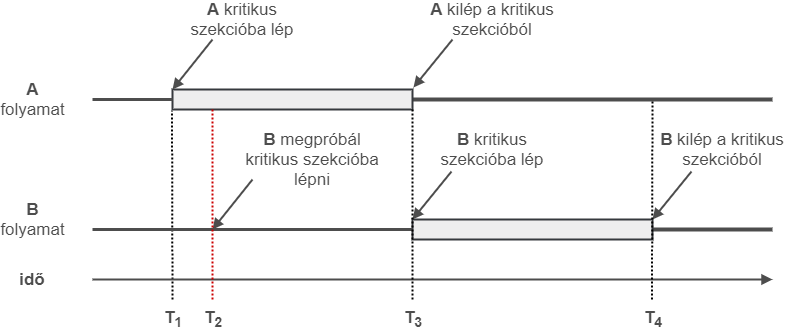
\includegraphics[width=0.9\textwidth]{img/mutex.png}
		\caption{A kölcsönös kizárás elvárt viselkedése}
	\end{figure}

    \noindent A két folyamat (az „A” és a „B” folyamatok) közti kölcsönös kizárás biztosítja, hogy egyidejűleg csak az egyik lehet a kritikus szekciójában. A „B” folyamat $T_2$ időpillanatban megpróbálja a kritikus szekcióját végrehajtani, de nem teheti, mert az „A” folyamat már a saját kritikus szekciójában van. A $T_2$ és  $T_3$ időpillanat között a „B” folyamatnak várakoznia kell arra, hogy be tudjon lépni a saját kritikus szekciójába.

	\subsection*{Megvalósítások}
	
    \subsubsection*{A kölcsönös kizárás biztosítása a megszakítások tiltásával}

    A legegyszerűbb megoldás a kölcsönös kizárás megvalósítására: a folyamat, mielőtt belépne a kritikus szakaszba, letiltja a megszakításokat, majd miután kilépett a kritikus szakaszból, újra engedélyezi a megszakításokat. Ezzel elérheti, hogy a kritikus szakasza alatt nem történik folyamatváltás, mivel az ütemező az óramegszakítás hatására cseréli le a folyamatokat. Ugyanezt éri el, ha csak az ütemezést vagy a folyamatváltást tiltja le a folyamat.\\

    \noindent Ez a megoldási módszer valódi párhuzamos folyamatok esetén nem használható, mivel a megszakítások tiltása csak az adott processzorra vonatkozik. Továbbá nem szabad a felhasználói folyamatoknak ekkora hatalmat adni, mivel a rosszindulatú folyamatok nem kapcsolják vissza a folyamatváltást, így átveszik az uralmat a processzor (CPU) felett.\\

    \noindent Az ismertetett megoldás a felhasználói programok esetén sem használatos, azonban a kerneleken belül gyakran alkalmazott módszer. A kernel a futása alatt tiltja a megszakításokat, így más folyamat nem futhat, amíg a kerneleljárás véget nem ért. Az egyprocesszoros rendszereknél így tudja biztosítani a kernelműveletek atomi voltát (megszakíthatatlanságát).\\

    \subsubsection*{Szigorú váltogatás}

    A következő megoldásban egy „zálog” nevű változó tartalmazza azt, hogy melyik folyamat léphet be a kritikus szakaszba.

\newpage
   \begin{verbatim}
#define FALSE 0
#define TRUE 1
int zalog;

while( TRUE ) {
     while( zálog != sorszámom );
     // Tevékeny várakozás.
     kritikus_szakasz();
     zálog = (zálog + 1) % folyamatok_száma;
     nem_kritikus_szakasz();
}\end{verbatim}

    \noindent A második sorban lévő ciklus azt teszteli, hogy beléphet-e a folyamat a kritikus szakaszba, azaz a zálog az ő sorszámával megegyezik-e. A ciklus magja egy üres utasítás, tehát csak a feltételt teszteljük folyamatosan. Ezt tevékeny várakozásnak nevezzük. A tevékeny várakozást általában kerülni kell, mivel nagyon pazarolja a processzor- (CPU-) időt. A másik probléma ezzel a megoldással, hogy a folyamatok sorba léphetnek csak be a kritikus szakaszba, ami megsérti a párhuzamos környezetben egy közös erőforrás használatakor javasolt feltételekből a harmadik feltételt, mivel ezáltal előfordulhat, hogy egy kritikus szakaszon kívüli folyamat sorszámával azonos a zálog, és ekkor ez a folyamat blokkolja a zálogra váró folyamatokat.\\

    \subsubsection*{Peterson megoldása (1981)}

    G. L. Peterson javította a szigorú váltogatást. Tegyük fel most azt, hogy két folyamat verseng egymással a közös erőforrás használatáért (processz = 0 és processz = 1). Mielőtt a folyamat belépne a kritikus szakaszba, meghívja a „belepes” eljárást, a kritikus szakasz végén pedig meghívja a „kilepes” eljárást. A „belepes” eljárás biztosítja, hogy szükség esetén várakozni fog a folyamat (mindezt tevékeny várakozással).

   \begin{verbatim}
#define FALSE 0
#define TRUE 1
#define N 2
int zalog;
int verseng[N];

while( TRUE ) {
     belepes(processz);
     kritikus_szakasz();
     kilepes(processz);
     nem_kritikus_szakasz();
}

void belepes(int proc) {
     int masik = 1 - proc;
     verseng[proc] = TRUE;
     zalog = proc;
     while(zálog == proc && verseng[masik] == TRUE);
     // Tevékeny várakozás.
}

void kilepes(int process) {
     verseng[process] = FALSE;
}\end{verbatim}

    \noindent A megoldás lényege az, hogy a \emph{verseng} nevű vektorban tároljuk azt, hogy mely folyamatok akarnak belépni a kritikus szakaszba. Ha csak az egyik folyamat akar belépni a kritikus szakaszba, akkor a \emph{zalog} az övé lesz, ha a másik folyamat nem verseng. Tehát a várakozó ciklust „átugorjuk”. Ha ezután a másik folyamat is belép, akkor a \emph{zalog} nála lesz, de a \emph{verseng} nevű vektorból azt látja, hogy a már belépett folyamat verseng, tehát várakozni fog addig, amíg a kritikus szakaszból ki nem lép a folyamat, és meg nem hívja a \emph{kilepes} eljárást. A \emph{kilepes} eljárás a \emph{verseng} nevű vektornak a folyamat sorszámával indexelt elemét FALSE-ra állítja.\\

    \paragraph*{A TSL utasítás használata}

    Szoftveres megoldás helyett hardveresen biztosított a kritikus szakaszba lépés.\\

    \noindent TSL (Test and Set Lock) utasítás, melynek működése a következő:
    \begin{verbatim}
boolean TSL (boolean & zár) {
    boolean érték = zár;
    zár = true;
    return érték;
}
    \end{verbatim}

    \noindent A TSL utasítástól elvárt, hogy legyen
        \begin{itemize}
            \item atomi
            \item megszakíthatatlan, és
            \item ugyanarra a zárra egyszerre csak egy processzor hajthatja végre
        \end{itemize}

    \noindent Ez által a szinkronizáció jóval egyszerűbbé válik:
    \begin{itemize}
        \item Belépés:
        \begin{verbatim}
    while (TSL(zár))
    ; /* várakozik */
        \end{verbatim}
        \item Kilépés:
        \begin{verbatim}
    zár = false;
        \end{verbatim}
    \end{itemize}

    \noindent A modern processzorokban általában van ilyen utasítás, viszont a \emph{korlátozott várakozás feltétele} nem teljesül!

    \subsubsection*{TSL + korlátozott várakozás}

    A várakozó folyamatok nyilvántartásával kijavítható a megoldásunk:

    \begin{itemize}
        \item Belépés:
        \begin{verbatim}
#define FALSE 0
#define TRUE 1

várakozik[i] = TRUE;
while (várakozik[i] && TSL (zár))
; /* vár */
várakozik[i] = false;
        \end{verbatim}
        \item Kilépés:
        \begin{verbatim}
j = i + 1;
do {
    j = (j + 1) % n;
} while (j != i && !várakozik[j]);
if (j == i)
    zár = false;
else
    várakozik[j] = false;
        \end{verbatim}
    \end{itemize}

    \noindent Ez már mindhárom követelménynek eleget tesz (kölcsönös kizárás, haladás, korlátozott várakozás).

    \paragraph*{Az alvás-ébredés módszere}

    Az előzőekben említett megoldások komoly problémájának róható fel az, hogy tevékeny várakozással oldották meg a problémát, azaz egy ciklusban vizsgálták, hogy beléphetnek-e a kritikus szakaszba, vagy sem. Ezzel a módszerrel feleslegesen sok processzor- (CPU-) időt pazaroltak. A tevékeny várakozás a processzoridő pazarlása mellett fordított prioritási problémának nevezett hibalehetőséget is magában rejti. Tegyük fel, hogy az operációs rendszer prioritásos ütemezőt használ. Amíg van magas prioritású futásra kész folyamat, addig alacsonyabb prioritású folyamatot nem futtat. Legyen egy alacsony prioritású folyamat, amelyik a kritikus szekciójában van; ekkor egy magas prioritású folyamat tevékeny várakozásba kezd, amit az alacsonyabb prioritású folyamat tudna feloldani, ha be tudná fejezni a kritikus szekcióját, de soha nem kerül a processzorhoz, mivel az ütemező mindig a magas prioritású tevékenyen várakozó folyamatot választja.\\

    \noindent A tevékeny várakozás feloldására javasolt egyik eszköz a sleep-wakeup páros. A sleep egy olyan rendszerhívás, amely blokkolja a hívó folyamatot, a wakeup pedig olyan rendszerhívás, amely felébreszti a paraméterül kapott alvó folyamatot.

    \paragraph*{Példa az alvás-ébredés módszerére: a gyártó-fogyasztó probléma}

    A sleep-wakeup használatára tekintsük példaként a gyártó-fogyasztó problémát. Van egy gyártó és egy fogyasztó folyamatunk. A gyártó termel, és a termelt árut elhelyezi egy tárolóban.\\ A fogyasztó fogyaszt úgy, hogy a tárolóból kiveszi az árut. A tároló kapacitása véges
    \begin{itemize}
        \item ha megtelik, a gyártást le kell állítani;
        \item ha kiürül, a fogyasztónak várnia kell, amíg újra áru kerül a tárolóba.
    \end{itemize}

    \noindent Amikor a gyártó egy új árut rak a tárolóba, és a tároló megtelik, akkor elmegy aludni, majd amikor a fogyasztó kivesz árut a tárolóból, akkor felébreszti a gyártót. Fordítva is hasonlóan: amikor a fogyasztó szeretne kivenni árut a tárolóból, de azt látja, hogy kiürült, akkor elmegy aludni, majd amikor a gyártó árut helyez el a tárolóban, akkor felébreszti az alvó fogyasztót.\\

    \noindent Legyen egy „DB” nevű változó, amely a tárolóban lévő elemek számát, illetve egy „KAPACITÁS” nevű változó, ami a tároló kapacitását tartalmazza.
\newpage
\begin{verbatim}
#define KAPACITAS 100
int DB = 0

void gyarto() {
     while(1) {
          gyart();
          if(DB == KAPACITAS)  // Megnézi, hogy tele van-e a tároló?
               sleep();        // Ha igen, akkor elmegy aludni.
          berak();             // Felébresztették, tehát berakhatja az árut.
          DB = DB + 1;         // A gyártó berakott egy árut a tárolóba.
          if(DB == 1)          // Ha üres volt a tároló,
               wakeup();       // akkor felébreszti a fogyasztót.
     }
}

void fogyaszto() {
     while(1) {
          if(DB == 0)          // Megnézi, hogy üres-e a tároló?
               sleep();        // Ha igen, akkor elmegy aludni.
          kivesz();            // Felébresztették, tehát kivehet egy árut.
          DB = DB - 1;         // A fogyasztó kivett egy árut a tárolóból.
          if(DB == N - 1)      // Ha tele volt a tároló,
               wakeup();       // akkor felébreszti a gyártót.
          feldolgozas();
     }
}
\end{verbatim}

    \noindent Versenyhelyzet előfordulhat ebben a megoldásban. Tegyük fel azt, hogy a tároló üres, és a fogyasztó kiolvassa a „DB” nevű változó értékét, majd az ütemező átadja vezérlést a gyártónak, aki betesz egy árut a tárolóba, és növeli a „DB” nevű változó értékét egyre. A gyártó látván azt, hogy a „DB” nevű változó értéke eggyel egyenlő (azaz DB==1), ébresztést küld a fogyasztónak, aki még nem alszik (tehát az ébresztés elmarad). Amikor a vezérlés visszakerül a fogyasztóra, a korábban kiolvasott „DB” nevű változó nulla értéke miatt (azaz DB==0) elmegy aludni. A gyártó szép lassan megtölti a tárolót, majd elmegy ő is aludni. Ezt követően mindkét folyamat alszik, és a másikra vár, hogy felébressze. Tehát így „örökké” aludni fognak. A probléma akkor történt, amikor a nem alvó folyamatnak küldtek ébresztést. Ez az ébresztés elveszett. Meg lehetne oldani, hogy az ilyen ébresztést elrakjuk, és amikor el akarna aludni a folyamat, akkor megnézi, van-e talonba ébresztése; ha igen, akkor nem alszik el, csak a talont felhasználja.
\newpage
    \subsubsection*{Sorszámhúzásos szinkronizáció}

    A  sorszámhúzós szinkronizáció tetszőleges számú folyamatra alkalmazható. Működése az ügyfélfogadó rendszerek mintájára épül.

    \noindent Implementáció: kezdetben sorszám[1..n] = 0
        \begin{itemize}[topsep=8pt,itemsep=4pt,partopsep=4pt, parsep=4pt]
            \item Belépés (i. folyamat):
            \begin{verbatim}
    sorszámot_húz[i] = TRUE;
    sorszám[i] = max(sorszám[1..n]) + 1;
    sorszámot_húz[i] = FALSE;
    for (j = 0; j < n; j++) {
        while (sorszámot_húz[j]); /* vár */
        while (sorszám[j] != 0 && (sorszám[j], j) < (sorszám[i], i))
        ; /* vár */
    }
        \end{verbatim}
            \item Kilépés:
            \begin{verbatim}
    sorszám[i] = 0;
            \end{verbatim}
        \end{itemize}

    \noindent Ez mindhárom követelménynek eleget tesz (kölcsönös kizárás, haladás, korlátozott várakozás).

	\section*{Szemaforok, osztott memória, üzenetküldés}
	
    \subsubsection*{Szemaforok}

    E.W. Dijkstra(1965) javasolta ezen új változótípus bevezetését. A szemafor egy új, egész értékű típus. Általános célú megoldás, a szinkronizáció megkönnyítésére.

    \begin{itemize}[topsep=8pt,itemsep=4pt,partopsep=4pt, parsep=4pt]
        \item Ha a szemafor értéke $> 0$, szabad a pálya, beléphetünk a kritikus szakaszra.
        \item Két atomi művelet (plusz kezdőértékadás)
        \begin{itemize}
            \item Ha belépünk egy kritikus szekcióba, csökkentjük szemafor értékét;
            \begin{itemize}
                \item \emph{down}(S): Ha S értéke zérus, várakozik, míg S pozitívvá nem válik. Egyébként, ill. ezután S-t eggyel csökkenti.\\
                (Eredetileg: P(S), a holland proberen, megpróbálni szóból.)
            \end{itemize}
            \item Ha kilépünk egy kritikus szekcióból, növeljük a szemafor értékét.
            \begin{itemize}
                \item \emph{up}(S): S értékét eggyel növeli. \\
                (Eredetileg: V(S), a holland verhogen, megemelni szóból.)
            \end{itemize}
            \item Megengedett, hogy egyszerre több down művelet legyen várakozó állapotban
        \end{itemize}
    \end{itemize}

    \noindent Ha a szemafor tipikus vasutas helyzetet jelöl, azaz 1 vonat mehet át csak a jelzőn, a szemafor értéke ekkor 0 vagy 1 lehet. Ez a \textit{bináris szemafor}, vagy más néven \textbf{\emph{mutexnek}} (Mutual Exclusion) nevezzük, és kölcsönös kizárásra használjuk. \\

    \noindent Rendszerhívással, felhasználói szinten nem biztosítható a műveletek atomiságának megvalósítása. Művelet elején például letiltunk minden megszakítást. Ha több CPU van, akkor az ilyen szemafort védeni tudjuk a TSL utasítással. Viszont ezek a szemafor műveletek kernel szintű, rendszerhívás műveletek. A fejlesztői környezetek biztosítják.

    \subsubsection*{Szemaforok alkalmazásai}

    \begin{itemize}[topsep=8pt,itemsep=4pt,partopsep=4pt, parsep=4pt]
        \item Kezdetben legyen mutex = 1.
        \item Belépés: down(mutex);
        \item Kilépés: up(mutex);
        \begin{verbatim}
while (1) {
    down(mutex);
    kritikus_szekcio();
    up(mutex);
    nem_kritikus_szekcio();
}
        \end{verbatim}
        \item Tetszőleges számú folyamatra működik.
        \item Kölcsönös kizárás és a haladás feltétele teljesül.
        \item Korlátozott várakozás teljesítése az \emph{up} implementációjától függ.
        \item Ha mutex értékét \emph{k}-ról indítjuk, egyszerre legfeljebb \emph{k} darab folyamat lehet a kritikus szekcióban.
        \item Már két utasítás felcserélése is gondot okozhat.
    \end{itemize}

    \subsection*{Szemaforok implementációja}

    Egyszerű implementáció:
    \begin{itemize}[topsep=8pt,itemsep=4pt,partopsep=4pt, parsep=4pt]
        \item down(S):
        \begin{verbatim}
while (S <= 0); /* vár */
S = S-1;
        \end{verbatim}
        \item up(S):
        \begin{verbatim}
S = S+1;
        \end{verbatim}
    \end{itemize}
    \noindent Feltételezések:
    \begin{itemize}
            \item S értékváltoztatásai atomiak
            \item A \emph{down} műveletben a ciklusfeltétel hamissá válása és az értékcsökkentés együtt is oszthatatlan művelet
    \end{itemize}

    \noindent Általában processzorok speciális utasításai segítik az implementációt.\\

    \noindent A szemafor és a mutex közti különbség: Az a különbség, hogy míg utóbbi csak kölcsönös kizárást tesz lehetővé, azaz egyszerre mindig pontosan csakis egyetlen feladat számára biztosít hozzáférést az osztott erőforráshoz, addig a szemafort olyan esetekben használják, ahol egynél több - de korlátos számú - feladat számára engedélyezett a párhuzamos hozzáférés

    \subsection*{Monitorok}

    A szemaforral ellentétben a monitor egy magasabb szintű, objektum elvű, objektumorientált művelet. Ezt a programszerkezetet C.A.R Hoare angol programfejlesztő  dolgozta ki 1974-ben. \

    \noindent A monitor objektum egy több szál által használt eljárás nem párhuzamos végrehajtását teszi lehetővé, azaz nem folyamat szintű művelet. Ötvözi az objektum orientált programozást a szinkronizációs metódusokkal.\\

    \noindent A monitor objektuma következőkből áll:

    \begin{itemize}[topsep=8pt,itemsep=4pt,partopsep=4pt, parsep=4pt]
        \item osztott adat
        \item ezeket az adatokat feldolgozó eljárások
        \item monitort inicializáló metódusok
    \end{itemize}

    \noindent A megvalósításhoz három dologra van szükség:

    \begin{itemize}[topsep=8pt,itemsep=4pt,partopsep=4pt, parsep=4pt]
        \item feltételváltozó és
        \item két művelet
        \begin{itemize}
            \item wait(): Az állapot bekövetkeztére vár, eközben más folyamatok is beléphetnek a monitorba
            \item signal(): Jelzi az állapot bekövetkeztét. Ha nincs az állapotra váró folyamat, nem csinál semmit; egyébként kiválaszt egy várakozó folyamatot, és felébreszti
        \end{itemize}
    \end{itemize}

    \noindent A  kritikus  adatokhoz  csak  szinkronizált  műveleteken keresztül lehet hozzáférni.\\

    \noindent Minden eljárás halmazt egy monitor kontrolál. A többszálas alkalmazás futásakor, a monitor egyetlen szálnak engedélyezi egy adott időpontban az eljárás végrehajtását. Ha egy szál  éppen egy monitor által kontrolált eljárást akar futtatni akkor az lefoglalja a monitort. Abban az esetben ha a monitor már foglalt akkor a belépni szándékozó szál várakozik amíg  a monitort lefoglaló szál befejezi az adott eljárás végrehajtását és felszabadítja a monitort.\\

    \noindent Előnye, hogy a közösen használandó erőforrások és az erőforrásokon végrehajtható műveletek egyetlen szintaktikus egységben helyezkednek el.\\

    \noindent A monitor és a szemafor összehasonlítása:
    \begin{itemize}[topsep=8pt,itemsep=4pt,partopsep=4pt, parsep=4pt]
        \item A monitor magasabb szintű eszköz. Magas szintű, objektumorientált nyelvek esetében (pl. Java) roppant egyszerűen használható.
        \item A szemaforok segítségével rugalmasabban kezelhetők a kritikus szakaszok, hiszen nem kell beágyazott módon, előre elkészíteni az összes kritikus szakaszt.
        \item A szemaforokkal több kritikus erőforrás használatát könnyebb általában összekombinálni egy kritikus szakaszon belül.
    \end{itemize}

    \noindent Ha olyan osztott, többprocesszoros rendszert használunk, ahol a központi egységeknek saját memóriájuk van, akkor ezek a módszerek nem igazán használhatóak.

    \paragraph*{Az üzenetküldéses paradigma}

    Ha a párhuzamos programot – a programfejlesztés valamilyen szintjén – egymástól független, egymással kommunikáló szekvenciális folyamatok halmazaként fogjuk fel,  akkor  a  kommunikációt  tekintve  alapvetően  kétfajta  programozási  paradigmáról beszélhetünk.

    \noindent Az első az osztott memóriás modell, amelyben a futó folyamatok ugyanahhoz a (nem feltétlenül fizikai) memóriához férnek hozzá.\\

    \noindent A második pedig az üzenetváltásos modell, amelyben minden egyes folyamat a többi által nem elérhető memóriát használ, a kommunikációt pedig a folyamatok közötti (szinkron, aszinkron, illetve a kettő közötti átmenetnek  megfelelő)  üzenetek  biztosítják.\\

    \noindent Az, hogy a programfejlesztési modellünk üzenetváltásos modell, nem jelenti feltétlenül azt, hogy végül az implementált programnak is feltétlenül „üzenetváltásos” hardveren kell futnia.\\
    Természetesen igaz az, hogy az üzenetváltásos modellnek megfelelő algoritmusok, programok  egyszerűbben  és  általában  hatékonyabban  implementálhatók  üzenetváltásos architektúrákon.  (Valamint  az  osztott  memóriás  modell  alapján  készült  programok egyszerűbben és hatékonyabban implementálhatók osztott memóriás hardveren.)

	\subsection*{Osztott memória}

    A megosztott memória segítségével megoldható, hogy különböző folyamatok ugyanazt a \lword{memóriaterületet} közösen használják. A közösen használt memóriaterület lehetőséget ad az adatok megosztására és a gyors kommunikációra. A rendszer csak a hozzáférési jogosultságokat kezeli, tehát az egyidejű közös erőforrás-használat következményeként versenyhelyzet alakulhat ki. A versenyhelyzetek kezelése a felhasználói folyamatok feladata.\\

    \noindent Közös memórián keresztül történő adatcsere esetén az együttműködő folyamatok mindegyike saját címtartományában lát egy közös memóriát. A közös memória elérését (a közös memória címtartományára kiadott olvasás vagy írás művelet végrehajtását) valamilyen adatátviteli rendszer (kapcsolóhálózat, sín stb.) teszi lehetővé.\\

    \noindent A folyamatok párhuzamos futása miatt a közös memóriát egyidejűleg több folyamat is írhatja, illetve olvashatja. Ilyen esetekre a RAM-modell nem határozza meg a memória működését, ezért a közös memóriát a RAM-modell kiterjesztésével kapott PRAM (Pipelined Random Access Memory) modell szerint kell kialakítani.\\

    \begin{figure}[H]
        \centering
        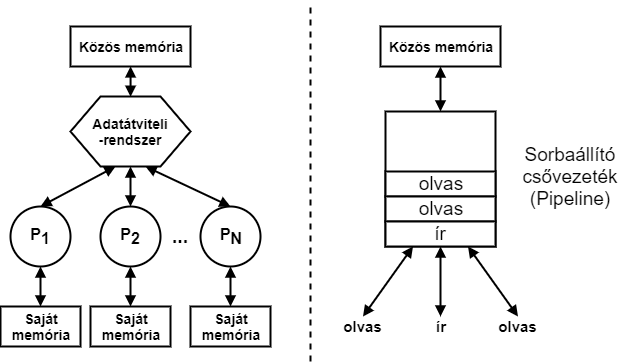
\includegraphics[width=0.7\textwidth]{img/shared_memory_sync.png}
        \caption{Folyamatok együttműködése PRAM szerint működő közös memórián}
        \label{shared_memory_sync}
    \end{figure}
\newpage
    \noindent A PRAM-modell szerint működő memóriát több processzor írhatja és olvashatja egyidejűleg. Az olvas és ír műveletek egyidejű végrehajtására a RAM-modellhez képest az alábbi kiegészítések vonatkoznak:
    \begin{itemize}
        \item olvasás-olvasás ütközésekor mindkét olvasás ugyanazt az eredményt adja, és ez megegyezik a rekesz tartalmával,

        \item olvasás-írás ütközésekor a rekesz tartalma felülíródik a beírni szándékozott adattal, az olvasás eredménye vagy a rekesz régi, vagy az új tartalma lesz, más érték nem lehet,

        \item írás-írás ütközésekor valamelyik művelet hatása érvényesül, a két beírni szándékozott érték valamelyike írja felül a rekesz tartalmát, harmadik érték nem alakulhat ki.
    \end{itemize}

    \noindent Ezek a szabályok lényegében azt jelentik, hogy az egyidejű műveletek nem interferálhatnak, azaz nem lehet közöttük zavaró kölcsönhatás. Hatásuk olyan lesz, mintha valamilyen előre nem meghatározható sorrendben hajtódnának végre (ezt tükrözi a pipelined elnevezés, arra utalva, hogy a memóriához egy sorosítást végző csővezetéken jutnak el a parancsok). Másként fogalmazva, ezek a műveletek a modell szintjén oszthatatlanok (atomiak).\\

    \noindent A közös memória használatával történő adatcsere helyes lebonyolításához a PRAM-modell szerint működő memória mellett a folyamatok működésének összehangolása is szükséges (például az adat fogadója akkor olvassa el az adatot, ha a küldő már elhelyezte azt; összetett adatok átadásakor félig átírt rekordot ne kezdjen olvasni a fogadó stb.). Ez ismét a folyamatok szabadon futásának (aszinkronitásának) korlátozását jelenti, azaz szinkronizációt igényel.
	
	\subsection*{Üzenetküldés}
	
    Üzenetváltásos adatcsere esetén a folyamatoknak nincs közös memóriája. Az adatátviteli rendszer most a logikai processzorokat kapcsolja össze. Rajta keresztül a folyamatok üzeneteket tudnak küldeni, illetve fogadni. Az üzenetküldésre, illetve fogadásra a folyamatok logikai processzorainak utasításkészletében megfelelő utasítások állnak rendelkezésre. Legyenek ezek a Küld (Send) és a Fogad (Receive) műveletek.\\

    \noindent A $\text{Küld}(<\text{cím}>,<\text{folyamat}>)$ művelet végrehajtásakor a műveletet végrehajtó folyamat elküldi a saját memóriájának megadott címén tárolt adatot a megadott folyamatnak,\\ a $Fogad(<\text{cím}>,<\text{folyamat}>)$ művelet pedig végrehajtásakor a megadott folyamattól érkező üzenetet a saját memória megadott címén tárolja.

    \begin{figure}[H]
        \centering
        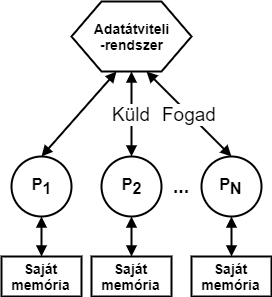
\includegraphics[width=0.35\textwidth]{img/messaging_sync.png}
        \caption{Folyamatok együttműködése üzenetváltással}
        \label{messaging_sync}
    \end{figure}

    \noindent Míg gyakorlatilag valamennyi közös memóriás információcserét alkalmazó megoldás a PRAM-modellre alapul, az üzenetközvetítésre nincs egyetlen elfogadott modell. Ha csak a működés logikájával foglalkozunk, és olyan lényeges kérdéseket nem is érintünk, mint az átviteli sávszélesség, az összeköttetés megbízhatósága, az üzenetszerkezet, az átviteli közeg sajátosságai, a kapcsolatépítés esetleges dinamikája, akkor is számos tulajdonságot találunk, amelyekben az egyes megoldások eltérhetnek, és amelyek ismerete fontos a felhasználók (rendszertervezők, programozók, üzemeltetők) számára. A folyamatok kommunikációs műveleteinek tulajdonságaival ezért külön pontban foglalkozunk.

    \subsection*{Folyamatok kommunikációja}

    A folyamatok együttműködésének másik alapmodellje a közös memóriás együttműködés mellett az üzenetváltásos együttműködés, azaz a folyamatok közötti kommunikáció. Az üzenetváltásos együttműködés akkor került előtérbe, amikor realitássá vált több, adatátviteli vonalon, vagy hálózaton keresztül összekapcsolt számítógép együttműködése.

    \noindent Azonkívül, hogy a logikai processzor utasításkészletében szerepel \emph{Küld} és \emph{Fogad} művelet, a kommunikáció működésével, tulajdonságaival kapcsolatban számos nyitott kérdés maradt, és \lword{megállapítottuk}, hogy nincs egyetlen tiszta modell, amelyet a megoldások követnek.\\

    \noindent Néhány a legkézenfekvőbb kérdések közül:
    \begin{itemize}[topsep=8pt,itemsep=4pt,partopsep=4pt, parsep=4pt]
        \item Milyen megnevezést használhatnak a kommunikáló partnerek, hogy egymásra találjanak?
        \item Milyen szemantikai konzisztenciának kell fennállni a küldés és a fogadás között?
        \item Milyen járulékos (implicit) szinkronizációs hatása van a kommunikációnak?
    \end{itemize}

    \paragraph*{A partner megnevezése}

    Megnevezés tekintetében beszélhetünk közvetlen (direkt), közvetett (indirekt), valamint aszimmetrikus kommunikációról, illetve megnevezésről, továbbá csoportkijelölésről és üzenetszórásról.\\

    \noindent A közvetlen (direkt) kommunikáció két folyamat között zajlik, mind a \emph{Küld}, mind a \emph{Fogad} művelet megnevezi a partner folyamatot (\ref{direct_communication}. ábra). $P_1$ elküldi a saját címtartományában tárolt $x$ változó értékét $P_2$-nek, aki azt saját $y$ változójába teszi el. (Ha a változók közös címtartományban lennének, egyszerűen $y:=x$ értékadást használhatnánk, így azonban kommunikációs műveletek szükségesek.)

    \begin{figure}[H]
        \centering
        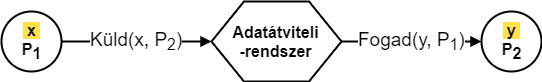
\includegraphics[width=0.6\textwidth]{img/direct_communication.png}
        \caption{Kommunikáció direkt megnevezéssel}
        \label{direct_communication}
    \end{figure}

    \noindent Közvetett (indirekt) kommunikáció esetén a partnerek nem egymást nevezik meg, hanem egy közvetítő objektumot, (például postaládát, vagy csatornát). A postaládán keresztül bonyolódó kommunikációt a \ref{indirect_communication}. ábra szemlélteti.

    \begin{figure}[H]
        \centering
        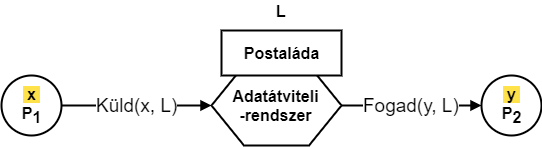
\includegraphics[width=0.6\textwidth]{img/indirect_communication.png}
        \caption{Kommunikáció indirekt megnevezéssel}
        \label{indirect_communication}
    \end{figure}

    \noindent A postaláda egy általában véges, de elméletileg esetleg korlátlan befogadóképességű, az üzenetek sorrendjét megtartó (FIFO) tároló, amely a \emph{Küld}-\emph{Fogad}, (betesz-kivesz) műveletpárral kezelhető. A $\text{Küld}(<\text{cím}>,<\text{postaláda}>)$ művelet a saját címtartományban elhelyezkedő üzenetet a postaláda következő szabad tárolóhelyére másolja. Ha a postaláda tele van, ürülésig várakozik. A $\text{Fogad}(<\text{cím}>,<\text{postaláda}>)$ művelet a postaládában legrégebben várakozó üzenetet kimásolja a megadott, saját címtartománybeli címre, helyét pedig felszabadítja.\\

    \noindent A csatorna olyan kommunikációs objektum, amelyik két folyamatot kapcsol össze. A csatorna lehet egyirányú (szimplex), osztottan kétirányú, azaz egyidejűleg egyirányú, de az irány változtatható (félduplex), vagy kétirányú (duplex). Tartalmazhat 0, véges vagy végtelen kapacitású átmeneti tárolót. Egy véges tárolókapacitású duplex csatorna egyenértékű két véges befogadóképességű postaládával, amelyeket csak két folyamat használ, egyiket egyik irányú, másikat az ellenkező irányú adatcserére.\\

    \noindent A postaláda és a csatorna lazítja a kommunikáló folyamatok közötti csatolást, lehetővé teszi, hogy olyan folyamatok is információt cseréljenek, amelyek nem ismerik egymást.

    \begin{figure}[H]
        \centering
        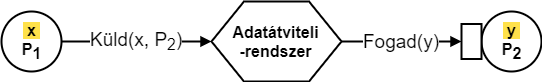
\includegraphics[width=0.6\textwidth]{img/asymmetric_communication.png}
        \caption{Kommunikáció asszimetrikus megnevezéssel}
        \label{asymmetric_communication}
    \end{figure}

    \noindent Aszimmetrikus megnevezés esetén az egyik folyamat, az adó vagy vevő, megnevezi, hogy melyik folyamattal akar kommunikálni, a másik partner viszont egy saját be-/kimeneti kaput (port) használ, amelyiket – ha csak egy van – nem is kell megneveznie. Ha az üzenet vevője használ bemeneti kaput, akkor a műveletek alakja $\text{Küld}(<\text{cím}>,<\text{folyamat}>)$, $\text{Fogad}(<\text{cím}>)$. Ez a megoldás azokban az esetekben hasznos, amikor a fogadó folyamat nem ismeri a küldőt, de a küldő ismeri a fogadót, például egy ügyfél folyamat szolgáltatási kérelmet küld egy szolgáltató folyamatnak (kliens–szerver modell). A fordított irányú aszimmetria alkalmazására pedig egy feladat lebontását és szétosztását végző menedzser folyamat és több, munkáért versengő végrehajtó folyamat kapcsolata lehet példa. A küldő a kimeneti port­jára küldi az elvégzendő feladatot tartalmazó üzenetet, a fogadó pedig az első ráérő feldolgozó lesz (farmer–worker modell).\\

    \noindent Csoportkommunikáció esetén az üzenet küldője folyamatok (esetleg kommunikációs objektumok) egy csoportját nevezheti meg vevőként. Ilyenkor egyetlen üzenetküldő művelet végrehajtása azt eredményezi, hogy az üzenetet a csoport valamennyi tagja megkapja. Az üzenetszórás (broadcasting) logikailag a csoportkommunikáció azon esete, amikor az egyetlen művelettel elküldött üzenet a rendszer valamennyi folyamatához eljut (\ref{broadcasting_communication}. ábra).\\

    \begin{figure}[H]
        \centering
        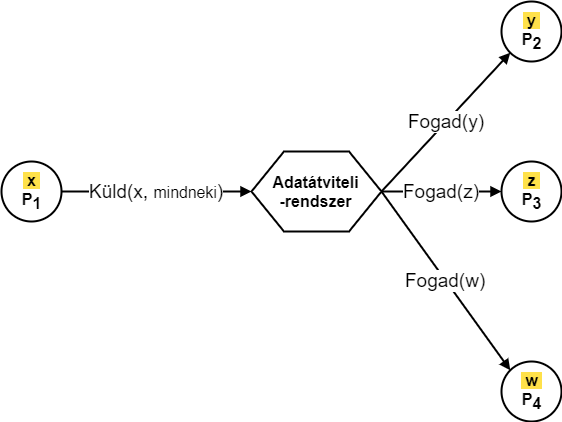
\includegraphics[width=0.6\textwidth]{img/broadcasting_communication.png}
        \caption{Kommunikáció üzenetszórással}
        \label{broadcasting_communication}
    \end{figure}

    \noindent A csoportkommunikáció lehetősége lényegesen egyszerűsíti a küldő műveleteit, ha több folyamattal akarja ugyanazt az információt közölni. Bizonyos típusú fizikai átviteli közegeken a csoportkommunikáció igen hatékonyan valósítható meg (például sín-topológiájú összeköttetések, \lword{rádiókommunikáció}).

    \paragraph*{Szemantikai konzisztencia}

    Most azt szeretnénk tisztázni, hogy mi történik a kommunikációs műveletek végrehajtásakor, milyen hatása van a műveleteknek az egyes folyamatok ál­la­­potterére (változókra, kommunikációs objektumokra), milyen minimális kon­zisztencia-feltételt kell betartani a műveletek megvalósításakor.\\

    \noindent Az üzenetváltásos modell akkor került előtérbe, amikor több számítógépet kapcsoltak össze egy rendszerré adatátviteli vonalon, vagy hálózaton keresztül. Ilyenkor fel kell készülni olyan rendkívüli esetekre is, hogy a partner folyamatot futtató számítógépet esetleg kikapcsolták, vagy a nagyobb távolságot áthidaló átvitel közben az adatok sérülnek, hiszen a hibalehetőség lényegesen nagyobb, mint az egyetlen chipben, dobozban, esetleg egyetlen kártyán elhelyezkedő egységek közötti átvitel esetén.\\

    \noindent Az üzenettovábbítás műveleteivel szemben ezért elvárás, hogy a műveletet végrehajtó folyamat ne fagyjon be sem átviteli hibák, sem a partner folyamatok kiesése esetén, és a kommunikációs műveletek helyes vagy hibás végrehajtásáról szerezzen tudomást.\\

    \noindent A műveletek helyességének visszajelzésére az egyik szokásos megoldás egy állapotkód visszaadása, amelynek egyik értéke a helyes végrehajtás, további értékei pedig az előforduló hibakódok lehetnek.\\

    \noindent Egy másik megoldás lehet a logikai processzor szintjén megvalósított hiba-megszakítás, ami a folyamat végrehajtását a hiba felderítéséhez és a folyatáshoz szükséges információk tárolását követően egy hibakezelési pontra (exception handler) irányítja. A partner folyamat kiesését szokásosan a műveletekre megszabott időkorlát (time-out) figyelésével észlelik. A kommunikációs művelet az időkorlát elérésekor hibajelzéssel akkor is befejeződik, ha a partner válaszának hiánya, vagy a kommunikációs közeg hibája miatt az adatcsere még nem történt meg. A folyamatok programozásához megfelelő rugalmasságot nyújt, ha lehetőség van a kommunikációs műveletekre vonatkozó időkorlát paraméterként történő megadására.\\
\newpage
    \noindent A hibajelzéssel és időkorláttal kiegészítve közvetlen kommunikáció esetén a műveletek a következő alakúak:
    \begin{itemize}[topsep=8pt,itemsep=4pt,partopsep=4pt, parsep=4pt]
        \item $\text{Küld}(<\text{cím}>,<\text{folyamat}>,<\text{időkorlát}>, <\text{hibakód}>)$, illetve
        \item $\text{Fogad}(<\text{cím}>,<\text{folyamat}>,<\text{időkorlát}>,<\text{hibakód}>)$.\\
    \end{itemize}

    \noindent Az időkorlát lehetséges értékei között célszerű a 0 és a <végtelen> értéket is megengedni. A 0 várakozás például akkor hasznos, ha egy fogadó folyamat működésének egy pontján csak akkor akar üzenetet fogadni, ha azt már elküldték, egyébként van más teendője. A $<\text{végtelen}>$ várakozás pedig az olyan folyamatok esetén szükséges, amelyiknek nincs teendője, amíg valaki egy üzenettel el nem indítja.\\

    \noindent A Küld művelet szemantikáját tekintve elsősorban az a kérdés merül fel, hogy okozhat-e várakozást a művelet, és mi az, ami az adatcseréből a művelet befejeződésekor, azaz a folyamat továbblépésekor már megtörtént.\\

    \noindent A lehetséges megoldásváltozatok közül az egyik véglet: a Küld művelet akkor fejeződik be, amikor az adatcsere teljes egészében befejeződött, a küldött üzenet rendben megérkezett és a helyére került. Ez a megoldás általában a \emph{Küld} művelet várakozását is okozhatja, a végrehajtás során ellenőrzések, esetleg hibajavítások is történhetnek. A megoldás ahhoz hasonló, mint amikor tértivevényes levelet küldünk valakinek, és addig nem lépünk tovább, amíg a tértivevény aláírva vissza nem érkezett.\\

    \noindent A másik véglet az lehet, hogy a Küld befejeződésekor az üzenet csupán bekerült a kommunikációs rendszerbe, de további sorsáról semmit sem tudunk. Ilyenkor a Küld művelet általában sohasem várakozik. Ez a megoldás ahhoz hasonló, mint amikor valakinek úgy küldünk levelet, hogy egyszerűen bedobjuk a postaládába, és továbbmegyünk.\\

    \noindent A két véglet között számos köztes megoldás létezhet (például az üzenet elhagyta azt a processzort, amelyiken a küldő folyamat fut stb.).\\

    \noindent Valamennyi megoldás esetén be kell tartani azt a minimális konzisztencia-feltételt, hogy amennyiben nincs hibajelzés, az elküldött üzenetet tartalmazó terület a küldő folyamat saját memóriájában (a $<\text{cím}>$ tartalma) a \emph{Küld} befejeződése után – akár a következő utasítással – felülírható legyen. Ennek már nem szabad hatással lennie az elküldött üzenetre.\\

    \noindent A \emph{Fogad} művelet megvalósításai általában várakozást okozhatnak abban az esetben, ha még nem érkezett üzenet. A művelet egyszeri végrehajtása pontosan egy üzenetet helyez el a fogadó folyamat saját memóriájába akkor is, ha esetleg több várakozó üzenet van a folyamat számára a kommunikációs rendszerben. Az üzenetek érkezési sorrendben fogadhatók, minden üzenet csak egyszer, azaz a fogadás törli az üzenetet a kommunikációs rendszerből. Postaláda, illetve bemeneti kapu használata esetén kérdés, hogy a fogadó tudomást szerez-e arról, hogy ki az üzenet küldője. Erre általában szükség van, hiszen az üzenetre gyakran választ kell küldeni. Ha a kommunikációs rendszer ezt az információt nem közli automatikusan, a folyamatoknak kell gondoskodniuk arról, hogy a küldő azonosítható legyen az üzenet tartalma alapján.\\

    \paragraph*{Járulékos (implicit) szinkronizáció}

    \noindent A kommunikációs műveletek általában a kommunikációban résztvevő folyamatok szabadonfutásának korlátozását okozzák. Az egyes műveletekkel járó szinkronizációs mellékhatás elsősorban a kommunikációs rendszer átmeneti tárolójának (puffer) kapacitásától függ.\\

    \noindent Tárolás nélküli átvitel esetén a kommunikációs rendszer csak közvetít, de a \emph{Küld} és \emph{Fogad} műveleteknek be kell várnia egymást ahhoz, hogy az információcsere megtörténhessen. A két folyamat ezen utasításaira egyidejűség érvényes (a \emph{Küld} és a \emph{Fogad} randevúja).\\

    \noindent Véges kapacitású tároló alkalmazása bizonyos keretek között kiegyenlíti a küldő és fogadó folyamatok sebességingadozásait. A fogadó folyamat várakozik, ha üres az átmeneti tároló, a küldő folyamat pedig akkor, ha nincs szabad hely a tárolóban. Ugyanazon üzenet elküldésének meg kell előznie az üzenet fogadását, tehát ezen műveletekre sorrendiség (precedencia) érvényesül. Emellett egy rövid távú szinkronizációs hatás is érvényesül, magának a tárolónak a kezelése általában kölcsönös kizárással valósul meg, azaz két folyamat ugyanazon kommunikációs objektumra hivatkozó kommunikációs műveleteinek megvalósítási részleteit szemlélve egyes szakaszokra kölcsönös kizárás áll fenn.\\

    \noindent Végtelen kapacitású tároló (csak modellben létezik) esetén a küldő folyamatnak sohasem kell várakoznia, egyébként a véges kapacitású tárolóra elmondottak érvényesek.
	
	\section*{Be- és kimeneti eszközök ütemezési lehetőségei, holtpontok}
	
	\subsection*{Be- és kimeneti eszközök ütemezési lehetőségei\\}
	
    Periféria kezelési módszerek:
    \begin{itemize}[topsep=8pt,itemsep=4pt,partopsep=4pt, parsep=4pt]
        \item Programozott
        \begin{itemize}
          \item közvetlen szoftver ütemezés
          \item lekérdezéses ütemezés
        \end{itemize}
        \item Megszakításos
        \item DMA
    \end{itemize}

    \subsection*{Programozott periféria kezelés\\}

    \paragraph*{Közvetlen szoftver ütemezés}

    \noindent Egyes  perifériáknál nincs szükség szinkronizálásra mert vagy nincs mihez szinkronizálódni (pl: egy kijelzőt meghajtó regiszter, egyszerű bementi port), vagy a periféria egy művelet elindítása után a következő utasítás végrehajtására már biztosan elkészül (gyors A/D konverter). Az ilyen perifériákhoz a processzor tetszőleges időpontban fordulhat.

   \paragraph*{Lekérdezéses ütemezés}

    \noindent Ha a periféria sebessége olyan, hogy egy perifériás művelet néhány utasítás végrehajtási időn belül fejeződik be, akkor a szinkronizálást státusz figyeléssel célszerű megoldani.

    \noindent Lassú periféria esetében sok várakozással jár , ami alatt a CPU nem végez érdemleges működést. Ezért csak akkor engedhető meg, ha CPU egyéb feladatait így is képes elvégezni . Az igényelt hardver tekintetében általában a lekérdezéses ütemezés a legolcsóbb megoldás.
\newpage
    \paragraph*{Program megszakításos periféria kezelés}

    Ha a periféria csak viszonylag hosszú idő vagy előre kiszámíthatatlan idő múlva lesz kész az újabb adatátvitelre, a lekérdezéses ütemezés feleslegesen foglalja a processzor idejét. Ezért ilyenkor interruptos periféria kezelést célszerű alkalmazni.\\

    \noindent A perifériához fordulást maga a periféria kezdeményezi egy logikai jellel a CPU vagy IT vezérlő interrupt kérő bemenetén. Az interruptot hardvertől függően az IT vonal szintje (szintérzékeny IT), vagy a jel valamely éle (élérzékeny IT) váltja ki.\\

    \noindent Az IT kezdeményezés hatására valamilyen mechanizmussal előbb-utóbb egy speciális szubrutinra (interrupt rutin) adódik a vezérlés, ami elvégzi a periféria kezelését . Mivel a CPU és a periféria szinkronizálása automatikus, nem kell feleslegesen státusz figyeléssel tölteni az időt.\\

    \noindent Az interruptos kezelés a program áttekinthetőségét is növeli . Mivel az IT rutinban nem a periféria kezelését szolgáló, ugyanakkor mindig végrehajtandó feladatok is vannak (regiszter mentés, regiszter visszaállítás, stack kezelés), túl sűrűn érkező IT-k szintén leronthatják a CPU kihasználtságát.

    \noindent IT-s periféria kezelést akkor célszerű alkalmazni, ha:
    \begin{itemize}[topsep=8pt,itemsep=4pt,partopsep=4pt, parsep=4pt]
        \item a CPU sebessége elegendő a periféria kezelésére és
        \item az interruptok várhatóan nem túl sűrűn jönnek , közöttük a CPU elég sok utasítást képes végrehajtani, vagy
        \item ha az interrupt bekövetkezésének időpontja véletlenszerű , de ha bekövetkezik, akkor gyorsan ki kell szolgálni,
        \item az interrupt alatt elvégzendő feladatok nem vesznek túl sok időt igénybe, vagy ha igen, akkor azt egyéb IT is megszakíthatja (többszintű IT rendszer).
        \item az interruptos szervezés a program strukturáltságát, áttekinthetőségét szolgálja.
    \end{itemize}

    \paragraph*{A közvetlen memória hozzáférés (DMA)}

    \begin{itemize}[topsep=8pt,itemsep=4pt,partopsep=4pt, parsep=4pt]
        \item Ha a processzor sebessége nem elegendő az adatátvitel lebonyolítására a periféria és memória között, DMA-s kezelést kell alkalmazni.
        \item Az ún. DMA vezérlő segítségével a processzort kikerülve, közvetlen adatátvitel lehetséges a memória és a periféria között. Ezt nevezik közvetlen memória hozzáférésnek (Direct Memory Access).
        \item A DMA átvitel általában gyorsabb, mintha a CPU végezné (nem kell közben a memóriából utasításokat olvasni és nem kell az adatot a CPU-n keresztül áramoltatni.
        \item A DMA-s kezelést tipikusan nagy sebességű, blokkos adatátvitelt igénylő perifériáknál alkalmazzák (winchester, nagysebességű soros adatátvitel stb).
        	\begin{itemize}
                \item \textit{Blokkos eszközök}: Adott méretű blokkban tároljuk az információt. Blokkméret 512 byte - 32768 byte között. Egymástól függetlenül írhatók vagy olvashatók. Blokkonként címezhetőek. Ilyen eszköz: HDD, szalagos egység
	        \end{itemize}
    \end{itemize}
\newpage
	\subsection*{Holtpontok (deadlock)}
	
    Két vagy több folyamat egy erőforrás megszerzése során olyan helyzetbe kerül, hogy egymást blokkolják a további végrehajtásban.\\

    \noindent \textbf{Definíció}. Folyamatokból álló halmaz \emph{holtpontban van}, ha minden folyamat valamelyik másik folyamat által kiváltható eseményre várakozik.\\

    \noindent A holtpontban lévő folyamatok tipikusan egy erőforrás felszabadítására várnak.\\

    \noindent Erőforrások például:

    \begin{itemize}[topsep=8pt,itemsep=4pt,partopsep=4pt, parsep=4pt]
        \item Szemaforral védett memóriaterület
        \item I/O eszközök
        \item Fájlok, rekordok olvasásának/írásának joga
        \item Processzorhasználat joga
        \item Új memóriaterület igénylése
    \end{itemize}

    \noindent Nem csak az I/O eszközökhöz kötődik, pl párhuzamos rendszerek, adatbázisok, stb. \\

    \noindent Az egyes erőforrástípusokból több példány is a rendelkezésre állhat. Mindegy, hogy melyiket kapja meg egy adott folyamat.\\

	\noindent Holtpont létrejöttéhez a következő négy feltételnek egyszerre teljesülnie kell:

	\begin{enumerate}[topsep=8pt,itemsep=4pt,partopsep=4pt, parsep=4pt]
		\item \textit{Kölcsönös kizárás.} Legyen legalább egy megoszthatatlan erőforrás
		\item \textit{Birtoklás és várakozás.} A folyamatoknak nem kell feladniuk az eddig megszerzett erőforrásokat ahhoz, hogy újakat igényelhessenek
		\item \textit{Megszakíthatatlanság.} Az erőforrások nem vehetők el a folyamatoktól a beleegyezésük (felszabadításuk) nélkül
		\item \textit{Ciklikus várakozás.} Lennie kell egy két vagy több folyamatból álló ciklikus listának, amiben minden folyamat a következő egy erőforrására várakozik
	\end{enumerate}

	\noindent Irányított gráffal lehet modellezni a folyamatokat és erőforrásokat. Ha van kör, akkor az holtpontot jelent. \\

    \subsection*{A holtpontok detektálása }

    A holtpontok detektálásához (észrevételéhez) az operációs rendszernek egyfolytában nyilván kell tartania azt, hogy hogyan osztotta eddig szét az erőforrásokat, mely folyamatoknak vannak ki nem elégített igényei. Ebből a nyilvántartásból kiindulva kell az operációs rendszernek felismernie a holtpont esetleges meglétét. Ehhez egy úgynevezett holtpontdetektáló algoritmust futtat le időnként.\\

    \noindent A holtpontdetektálás nem egyszerű feladat, mivel nem feltétlenül egy-két folyamat között alakulhat ki ilyen függőség, hanem akár jóval több folyamat is részt vehet egy holtpont kialakulásában, ami lehetséges, hogy „észre sem vehető”, mert nem befolyásol más, rendszer közeli folyamatokat.

    \subsection*{A holtpontok detektálásának stratégiája }

    A holtpontok detektálására adott lehetséges stratégia a következő:

    \begin{itemize}[topsep=8pt,itemsep=4pt,partopsep=4pt, parsep=4pt]
        \item A futó folyamatok közül pontosan azokat válogassuk ki, amely folyamatoknak van valamilyen erőforrásigényük. (Ezek lehetnek ugyanis olyan folyamatok, amelyek egy holtpont létrejöttében részt vehetnek!)
        \item Ezt követően a kiválogatott folyamatok közül keressük ki azokat, amelyeknek csak olyan erőforrásigényük van, ami éppen az adott pillanatban kielégíthető, azaz az erőforrás-kezelő a folyamatnak oda tudja adni az erőforrást, mert az éppenséggel szabad. Ezeket a folyamatokat jelöljük meg.
        \item Tekintsünk szabadnak minden olyan erőforrást, amit a most kijelölt folyamatunk használ.
        \item A második ponttól kezdve ismételgessük az algoritmust addig, amíg el nem jutunk egy olyan állapotba, amelyben már nincsen más kiszolgálható tevékenység.
    \end{itemize}

    \noindent Ha a holtpontok detektálására adott eljárás végén marad nem kiszolgálható folyamat, akkor az operációs rendszerben holtpont rejtőzik, és a hátra maradt folyamatok éppen azok a folyamatok, amelyek a holtpont kialakításában részt vesznek.\\

    \noindent Az algoritmusról könnyen belátható, hogy a holtpontok detektálására adott stratégia végén megkapott folyamatok halmaza nem függ attól, hogy az algoritmus elején melyik folyamatot választjuk ki elsőként.\\

    \noindent A holtpontdetektáló algoritmus egy úgynevezett „mohó” algoritmus, aminek a gyakori lefuttatása az operációs rendszer hatékonyságát csökkenti. Felmerülhet kérdésként ekkor az olvasóban: mi lehet vajon ennek az algoritmusnak az optimális aktivizálási ideje, azaz vajon milyen időközönként célszerű futtatnunk, hogy az operációs rendszer hatékonysága ne drasztikus mértékben csökkenjen?\\

    \noindent Erre egy egyszerű meghatározást lehet adni: célszerű azt a megoldást használni, hogy a holtpontdetektáló algoritmus akkor induljon el, ha egy folyamat olyan hosszú ideig várakozik egy erőforrás használatára, hogy már túllép egy előre meghatározott időintervallumot a várakozás.\\

    \subsection*{A holtpontok megszüntetése\\}

    \paragraph*{A drasztikus megszakítás}

    Ez a módszer úgy oldja meg a holtpont miatti konfliktust, hogy a várakozási körben található összes folyamatot megszakítja. Drasztikus módszer, mivel ebben az esetben a folyamatok eredményei is elvesznek, mivel a megszakítás miatt egyik sem fogja folytatni a tevékenységét.\\

    \paragraph*{A kevésbé drasztikus, kompromisszumos megoldások}

    \noindent Sokszor elég csak néhány tevékenységet megszakítani, és nem az összes folyamatot. Sőt, sok esetben nem is kell megszakítani ezen kiválasztott folyamatokat sem, hanem csak elég, úgymond, visszaállítani őket egy olyan állapotba, mielőtt a már korábban lefoglalt erőforrásra megadták volna az igénylésüket, és ezzel megnövelték a holtponthelyzet létrejöttének esélyét.\\
\newpage
    \noindent A következő módszerekkel megszüntethető az operációs rendszer által felismert holtpont kevésbé drasztikusan:
    \begin{enumerate}[topsep=8pt,itemsep=4pt,partopsep=4pt, parsep=4pt]
        \item módszer: Keressük meg azt a folyamatot, amelyik a „legaktívabban” vesz részt a holtpont kialakításában! Többnyire elegendő egyetlen egy ilyen „aktív” holtpont kialakító folyamat eltávolítása.
        \item módszer: Keressünk egy olyan folyamatot, amely újraindítható bármiféle mellékhatás nélkül! Természetesen egy adatmódosító művelet nem tekinthető újraindíthatónak, mivel lehet, hogy az újraindításával inkonzisztencia lépne fel az adatok között.
        \item módszer: Keressünk meg azokat a folyamatokat, amelyek újraindítása a legkevesebb költséggel jár! Tehát olyan folyamatokat, tevékenységeket keressünk ki, amelyek vagy olyan ellenőrzési pontokkal (checkpoint) rendelkeznek, amelyekre könnyen visszaállíthatóak, vagy éppen „most” kezdték meg működésüket, tevékenységüket.
        \item módszer: A holtpontot előidéző folyamatokat a prioritásuk szerint vizsgáljuk meg, és válasszuk ki a legalacsonyabb prioritású folyamatot, majd távolítsuk el, szakítsuk meg a működését, vagy állítsuk vissza valamilyen korábbi megfelelő állapotba, ha lehetséges.
    \end{enumerate}

    \noindent A holtpont megszüntető műveleteknél fontos, hogy a holtpont megszüntetésekor az automatikus választás mindig komoly kockázati tényezővel jár. A kockázat mellett figyelembe kell venni azt is, hogy bármilyen módszert választunk is ki a holtpont megszüntetésére, ugyanazt a folyamatot nem választhatjuk ki végtelen sokszor a holtponthoz kapcsolódó folyamatok „várakozási köréből” való eltávolítására, ugyanis ez az adott folyamat kiéheztetését okozná. Törekedni kell az optimális holtpontkezelésre, mivel a kiéheztetésen túl a holtpontkezelés legnagyobb veszélyei közé tartozik, ha az operációs rendszerünk alulszabályozott, vagy éppen túlszabályozott a holtpontdetektálással és a holtpont megszüntetéssel kapcsolatban.\\

    \noindent Alulszabályozás alatt azt kell érteni, hogy az operációs rendszer olyan nagyfokú túlbiztosítására törekszünk, hogy holtpont sosem alakul ki a futó folyamatok közt az operációs rendszerben, de magának a rendszernek a lehetőségeit sem fogjuk tudni kihasználni. Túlszabályozottság alatt pedig azt kell érteni jelen esetben, hogy olyan bonyolult holtpontdetektáló vagy éppen holtpontmegszüntető algoritmust választunk ki, hogy magának az algoritmusnak a végrehajtása lassítja az operációs rendszert, és csökkenti a rendszer hatékonyságát.

	\subsection*{Holtpontkezelés\\}

    \subsubsection*{Holtpont-megelőzés\\}

    A holtpontokat el tudjuk kerülni, ha garantálni tudjuk, hogy a holtpont létrejöttének négy feltételének valamelyike biztosan nem áll fenn.\\

    \noindent A holtpont kialakulásához szükséges feltételek elkerülése:

    \begin{itemize}[topsep=8pt,itemsep=4pt,partopsep=4pt, parsep=4pt]
        \item A \emph{\textbf{kölcsönös kizárás}} néhány esetben elkerülhetetlen, így ezekben az esetekben nem lehet mit csinálni, de más esetekben elkerülhető. Az egyik leggyakrabban használt technika az úgynevezett spooling technika (simultaneous peripherial operation on-line), ami annyit teszt, hogy a direkt erőforrás-használat helyett egy általában nagyméretű átmeneti tárolóba helyezzük az erőforrást.
        \item Az erőforrások lefoglalása (\emph{\textbf{Birtoklás és várakozás}}) úgy kerülhető el, ha elrendeljük azt, hogy egyszerre csak egy erőforrást foglalhat le egy folyamat, tehát egy folyamat csak akkor igényelhet egy új erőforrást, ha nem birtokol már egy másik erőforrást.

            \noindent Ezt kétféle módon érhetjük el:

            \begin{enumerate}
                \item Az összes szükséges erőforrást egyszerre kell igényelni, a folyamat indulásakor
                \begin{itemize}
                    \item Néha a program indulásakor még nem tudja, milyen erőforrásra lesz szüksége
                    \item Pazarló erőforrás-gazdálkodást eredményez
                \end{itemize}
                \item Új erőforrás igényléséhez el kell engedni az eddig megszerzetteket
                \begin{itemize}
                    \item Kiéheztetéshez vezethet
                    \item Kényelmetlen
                \end{itemize}
            \end{enumerate}
        \item A \emph{\textbf{„megszakítás nem megengedett”}} (\emph{Megszakíthatatlanság}) kiküszöbölése, azaz hogy nincs erőszakos erőforrás-elvétel, a következő módon érhető el: hogyha az erőforrásaink menthető állapotúak, akkor elvehetjük az adott folyamattól az erőforrás birtoklásának jogát úgy, hogy mentjük az erőforrás állapotát, majd az erőforrást átadjuk a másik folyamatnak, és mikor a másik folyamat befejezte a működését, akkor az erőforrás régebbi állapotát visszaállítva visszaadjuk az erőforrást az előző folyamatnak.
            \begin{itemize}
                \item Csak néhány erőforrástípus esetén alkalmazható. Például. processzor, fizikai memória, de I/O eszközök, fájlok esetén nem!
            \end{itemize}
        \item A \emph{\textbf{visszatérő igények}} (\emph{Körkörös kizárás}) elkerülése úgy érhető el, hogy kialakítunk egy hierarchikus rendszert. Az erőforrásokat kategorizáljuk, és hozzájuk prioritásokat rendelünk. Ez után minden folyamat csak olyan erőforrásokat igényelhet, amelyeknek a prioritása nagyobb, mint amilyen erőforrásai már vannak.

        \begin{itemize}
            \item Kizárjuk a hurkok lehetőségét
            \item Lehetetlen minden folyamatnak megfelelő sorrendet kitalálni
            \item Pazarló erőforrás-gazdálkodás
        \end{itemize}
    \end{itemize}

    \noindent A feltételek közül az első, illetve a harmadik feltétellel nem tudunk mit kezdeni, mivel az operációs rendszerünkben vagy vannak a feltételek által megállapított fajtájú erőforrások, vagy nincsenek.

    \subsubsection*{Holtpont-elkerülés}

    \paragraph*{A strucc algoritmus}

    A strucc algoritmus a „struccpolitika” elvét vallja, aminek egyszerűen a lényege az, hogy nem veszünk tudomást a holtpont létezéséről. Ha tudjuk azt, hogy egy esetleges holtpont kialakulásának valószínűsége meglehetősen kicsi, és az operációs rendszer újraindításának nincsenek kritikus következményei, akkor előfordulhat, hogy érdemes ezt a „megoldást” választani, mint holtpont „elkerülő” algoritmust.

    \begin{itemize}[topsep=8pt,itemsep=4pt,partopsep=4pt, parsep=4pt]
        \item \emph{Előnyei}:
        \begin{itemize}
            \item Gyors holtpontelkerülés.
        \end{itemize}
        \item \emph{Hátrányai}:
            \begin{itemize}
                \item Adatvesztés, a folyamatok végeredményeinek elvesztése fennállhat.
                \item Holtpontok megléte: mivel az algoritmus szerint csak figyelmen kívül hagyjuk a holtpontokat, azaz a holtponthelyzeteket, azok ugyanúgy ott lesznek, és maguktól nem fognak köddé válni.
                \item Kritikus következmények esetleges megléte.
                \item Nem ajánlott, mivel ez csak egy „struccpolitika”.
            \end{itemize}
    \end{itemize}

    \paragraph*{Egyetlen foglalási lehetőség stratégia (one-shot allocation strategy)}

    Az egyetlen foglalási lehetőség stratégia lényege az, hogy megtiltja a várakozás közben fellépő erőforrás-lekötést, azaz csak az a folyamat igényelhet magának erőforrást, amelyiknek egy \lword{erőforrásigénye} sincs.\\

    \noindent A stratégia alkalmazása esetén egy folyamat csak egyetlen alkalommal, általában a folyamat induláskor foglalhatja le azokat az erőforrásokat, amelyekre szüksége van a futása során. A stratégia alkalmat ad arra ezáltal, hogy ha a folyamat indulásakor van olyan erőforrás, amelyet a folyamat nem tud lefoglalni (tehát az adott erőforrás éppen nem szabad), akkor az operációs rendszer a folyamatot várakozásra kényszeríti, és így egy úgynevezett várakozási listára kerül fel. Ezen felül a stratégia még elrendeli azt is, hogy mivel egyetlen alkalommal foglalhatja le csak a folyamat a szükséges erőforrásokat, így a futása során más alkalommal nem nyújthat már be erőforrásigényt az operációs rendszer felé, és ha van is erőforrás-igénylése, akkor az operációs rendszer elutasítja, mivel már rendelkezik erőforrásokkal.\\

    \noindent Holtpont nem alakulhat ki az operációs rendszernek a futó folyamatai között, mivel a futó folyamatok minden erőforrást elérhetnek, amikre szükségük volt már a futásuk elején, mert ha valamilyen erőforrás megléte (birtoklása) hiányozna, akkor nem futó folyamatok lennének, hanem a várakozási listában várakoznának, illetve ezek a várakozó folyamatok nem rendelkeznek semmilyen erőforrás használatával.

    \begin{itemize}[topsep=8pt,itemsep=4pt,partopsep=4pt, parsep=4pt]
        \item Előnyök:
        \begin{itemize}
            \item Holtpont nem alakulhat ki a stratégia használata esetén.
            \item Ha egy folyamat már megszerezte az összes olyan erőforrást, ami a futásához szükséges, akkor biztosan nem kell sohasem várakoznia a futása során esetleges erőforrás-használat megszerzésére, így a folyamat futási idejét semmilyen erőforrásra való várakozás nem fogja megzavarni, meghosszabbítani.
        \end{itemize}
        \item Hátrányok:
        \begin{itemize}
            \item A folyamatoknak a futásuk végéig kell birtokolniuk a futásuk kezdetekor szükségessé vált erőforrásokat, tehát akkor is, ha nincsen rá semmilyen szükségük. Eszerint ez egy nagyon pazarló stratégia.
            \item Nem mérhető fel minden esetnem egy folyamat erőforrásigénye már a futás kezdetekor.
            \item Kiéheztetés lehetséges fennállása: ha egy folyamat nagyon sok erőforrást igényel, akkor előfordulhat, hogy nem mindegyik elérhető a futásának az elején, így lehetséges az, hogy beláthatatlan ideig várakozásra kényszeríti az operációs rendszer a folyamatot, így egyszerűen kiéheztetve az erőforrásokra vonatkozóan.
        \end{itemize}
    \end{itemize}

    \paragraph*{Rangsor szerinti foglalási stratégia (hierarchical allocation strategy)}

    \noindent A rangsor szerinti foglalási stratégia a ciklikus várakozási lehetőségét küszöböli ki azzal, hogy az erőforrásokat úgy kategorizálja, hogy minden egyes kategóriához egy-egy sorszámot rendel, és a leggyakrabban használt erőforráshoz a legkisebb sorszámot rendeli, míg a legritkábban használt erőforráshoz pedig a legnagyobb sorszámot, így felállítva közöttük egy úgynevezett prioritási sorrendet.\\

    \noindent A rangsor szerinti foglalási stratégia lényege a prioritási sorrend megkonstruálása által az, hogy a különböző folyamatok mindig csak növekvő sorszámú erőforrást igényelhetnek az operációs rendszertől, azaz egy folyamat mindig csak magasabb sorszámú erőforrást igényelhet meg az operációs rendszertől, mint amilyen sorszámú prioritást már birtokol.\\

    \noindent Továbbá, ha egy folyamatnak a meglévő erőforrásainak sorszámainál alacsonyabb sorszámú erőforrásra van szüksége, akkor fel kell szabadítania a szükséges erőforrás sorszámánál nagyobb sorszámú erőforrásokat egészen addig, míg a folyamat erőforrás-igénylési feltételei (lényegében a rangsor szerinti foglaláis stratégia feltételei) nem teljesülnek.

    \begin{itemize}[topsep=8pt,itemsep=4pt,partopsep=4pt, parsep=4pt]
        \item Előnyök:
        \begin{itemize}
            \item holtpont nem alakulhat ki a stratégia használata esetén.
            \item Nagyon hatékony, ha a megfelelő módon történt a sorszámok kiosztása az erőforrásoknak.
        \end{itemize}
        \item Hátrányok:
        \begin{itemize}
            \item Ha nem megfelelő módon történik a sorszámok kiosztása az erőforrásoknak, akkor nem biztosítható a stratégia hatékonysága.
            \item Problémás eset, ha a folyamatnak a meglévő erőforrásai sorszámainál alacsonyabb sorszámú erőforrásra van szüksége.
        \end{itemize}
    \end{itemize}

    \paragraph*{Bankár-algoritmus}

    Edsger Wybe Dijkstra-tól származik az egyik holtpontelkerülő ütemezési algoritmus, amit bankár algoritmusnak is nevezünk.\\

    \noindent Az algoritmus neve onnan származik, hogy a probléma nagymértékben hasonló a bankárok munkájához, azaz általánosabban tekintve a bankok erőforrás-kihelyezési problémájához. A hitelt igénylő ügyfelek a bankárhoz fordulnak a beruházásaik finanszírozásához szükséges hitelekért. A bankár az ügyfelek egy meghatározott (a hitelt kérő ügyfeleknek) csoportjával foglalkozik, akiknek folyósít egy bizonyos mennyiségű hitelt. A hiteligénylők a bankárnak megmondják, hogy pontosan mennyi lenne az a maximális pénzmennyiség, amire szükségük lehet, és a bankár ezt folyósítja számukra.\\

    \noindent Természetesen a bankár nem rendelkezik végtelen mennyiségű készpénzzel, így nem rendelkezik annyi pénzzel sem, ami az összes ügyfél teljes hiteligényét kielégítené egy időpontban. A hitelt csak az az ügyfél tudja visszafizetni, aki be is tudja fejezni a beruházását, amihez a hitelt igényelte eredetileg, ám a beruházás befejezéséhez szüksége van arra, hogy előbb vagy utóbb hozzáférhessen az igényelt hitel teljes pénzösszegéhez. A bankár tudja, hogy nem mindegyik ügyfélnek lesz szüksége azonnal a maximális hitelre, és feltételezi, hogy minden ügyféle a teljes hitel felvételét követően, amint csak tudja, azonnal vissza is fizeti a hitelt.\\

    \noindent A hitelt csak az az ügyfél tudja visszafizetni, aki be tudta fejezni a beruházást; ehhez pedig szüksége van arra, hogy előbb-utóbb hozzájusson az igényelt hitel teljes összegéhez.\\

    \noindent Ha a bankár nem elég óvatosan bánik a pénzével, akkor könnyen „megnézheti magát”, mivel kiürülhet a pénzes kasszája, és egyik ügyféle sem fejezné be a beruházását, mivel nem lenne egyiküknek sem pénze, amiből gazdálkodhatna, és folytathatná a beruházást, vagy akár törlessze a hitelt, mert nem kapná meg a hitelének a következő részét.\\

    \noindent Az algoritmus pontosan azt adja meg, hogy hogyan kell eljárnia a bankárnak az előbb említett (holtpont) helyzetek elkerülésére, feltételezve, hogy csak önmagára számíthat, és nincsen semmilyen segítsége, amire számíthatna?\\
\newpage
    \noindent A bankár algoritmus lényege tehát az, hogy az operációs rendszert mindig egy biztonságos állapotban tartja. A biztonságos állapot a bankár algoritmus esetében azt jelenti, hogy létezik legalább egy olyan erőforrás-igénylés kielégíthetőségi sorrend, amely szerint minden egyes folyamat erőforrás-igénylése kielégíthető. Tehát létezik olyan állapotsorozat, amelynek eredményeként mindegyik ügyfél felvehet összesen annyi kölcsönt, amennyit a hitel lehetősége enged, azaz minden folyamat megkapja az összes erőforrását, majd a tevékenysége után befejeződik. Az algoritmus sohasem elégít ki egy olyan erőforrás-igénylést sem, amely által az operációs rendszer biztonságos állapota nem állna fenn.\\

    \noindent A bankár algoritmus csak akkor működik, ha a folyamatok már az indulásukkor tudják, hogy a különböző erőforrásokból egyszerre maximálisan mennyit fognak igényelni, illetve ezt az operációs rendszernek be is jelentik.\\

    \noindent Ha az operációs rendszer állapota nem biztonságos, még nem jelenti azt, hogy a holtpont biztosan kialakul, hanem mindössze csak annyit jelent, hogy lehetséges holtpont kialakulása az adott állapotból. A bankár algoritmus úgy garantálja a holtpontmentességet, hogy már a nem biztonságos állapot kialakulását is megakadályozza, tehát a túlzott biztonságot tartja szem előtt. A módszer legnagyobb hátrányának tekinthető, hogy léteznek olyan folyamatok, amelyeknek erőforrásigénye előre nem ismerhető fel.\\

    \noindent A bankár algoritmus minden egyes erőforrás-igénylés megjelenésekor elemzést végez, és megnézi, hogy vajon az erőforrás-igénylés engedélyezése esetén is biztonságos marad-e a rendszer. Ha igen, akkor a kérést jóváhagyja, ha nem, akkor a kérést későbbre halasztja. Egy állapot biztonságosságának eldöntésekor a bankár azt elemzi, hogy van-e elegendő erőforrása ahhoz, hogy kielégítse néhány ügyfél hiteligényét. Ha ezt meg tudja tenni, akkor természetesen feltételezi, hogy az ügyfelek a kölcsönöket vissza fogják fizetni, és következhet annak az ügyfélnek a vizsgálata, akinek a hitelfolyósításainak összege a legközelebb van az általa igényelhető maximális hitelmennyiségnek, és így tovább. Ha az ügyfelek minden kölcsönt visszafizetnek a bankárnak, akkor az állapot biztonságos, és a kezdeti erőforrás igénylését a folyamatnak ki lehet elégíteni.
	
	\section*{Memóriakezelés, virtuális memória fogalma}
	
    Az alapvető memóriakezelési módszerek két csoportba sorolhatók:

    \begin{enumerate}[topsep=8pt,itemsep=4pt,partopsep=4pt, parsep=4pt]
        \item már a betöltéskor eldől, hogy mi hova kerül, és a futás végéig állandósul a memória, azaz a programon belüli esetleges dinamikus definíciókon kívül a memóriának a „programot” tartalmazó része állandó;
        \item végrehajtás közben mozgatják az egyes programrészeket a központi tár és a lemez között (lapozás, szegmentálás);
    \end{enumerate}

	\subsection*{Monoprogramozás}

    \noindent A legegyszerűbb memóriakezelési módszer, időben csak egyetlen programot futtatunk. Lényege, hogy a memóriát csak saját programunk, illetve az operációs rendszer között kell „felosztani”. \\

    \noindent Ezt a felosztást háromféleképpen végezhetjük – a sorrend a kisebb címtől a nagyobb cím felé haladást jelenti:  \\
    \begin{enumerate}[topsep=8pt,itemsep=4pt,partopsep=4pt, parsep=4pt]
        \item felhasználói program, operációs rendszer a RAM-ban – ezt a felosztást régi nagyszámítógépes rendszerekre, illetve miniszámítógépeken (Commodore, HT-1080Z) használták;
        \item operációs rendszer a RAM-ban, felhasználói program – főleg beágyazott rendszerek használják ezt a felosztást;
        \item eszközmeghajtók a ROM-ban, felhasználói program, operációs rendszer a RAM-ban – korai személyi számítógépekre jellemző. Lényegében a ROM-ba égetett rész nem más BIOS (Basic Input-Output System).
    \end{enumerate}

    \subsection*{Multiprogramozás\\}

    \subsubsection*{Multiprogramozás rögzített partíciókkal}

    \noindent Főleg kötegelt rendszerek tipikus megoldása.

    \begin{enumerate}[topsep=8pt,itemsep=4pt,partopsep=4pt, parsep=4pt]
        \item[1.] Különböző méretű partíciókat definiálunk és a megfelelő programot a hozzá méretben illeszkedő várakozási sorba rakjuk. Hátránya a megvalósításnak, hogy több várakozási sort (queue) kell nyilvántartani és menedzselni.

        \begin{figure}[H]
            \centering
            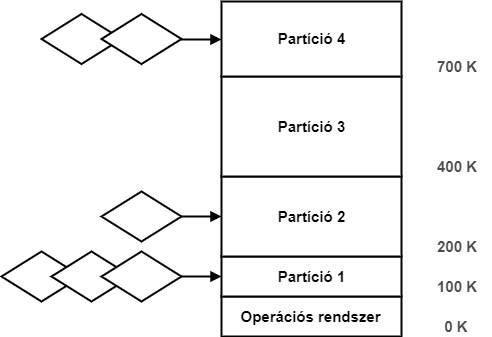
\includegraphics[width=0.5\textwidth]{img/memory_partitioning_individial_queue.png}
            \caption{}
            \label{memorymanagement_partitioning_iq}
        \end{figure}

        \item[2.] Csak egy várakozási sort használunk, ekkor a megüresedett partíció helyére az a program kerül, amelyik a sorban előrébb van és bele is fér a partícióba.

        \begin{figure}[H]
            \centering
            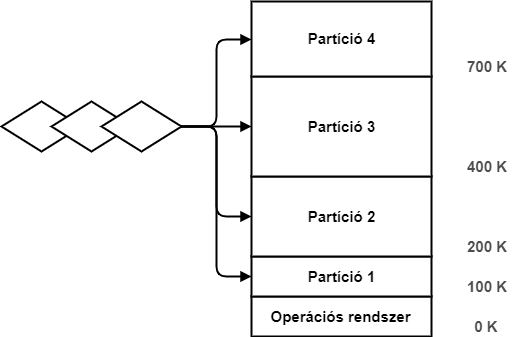
\includegraphics[width=0.5\textwidth]{img/memory_partitioning_single_queue.png}
            \caption{}
            \label{memorymanagement_partitioning_sq}
        \end{figure}

         Ebben az esetben kis módosítása lehet a kiválasztásnak, hogy nem az első beleférő programot helyezzük bele a partícióba, hanem a beleférők közül a legnagyobbat. Ezzel a módszerrel a partíció veszteséget lehet minimalizálni. \\

         Egy-egy programválasztás során a partícióba több program fér be, a nem kiválasztottakhoz jegyezzük fel, hogy most éppen nem volt szerencséjük. Ezt a \emph{szerencsétlenség} számlálót növeljük egyel. Megadhatunk egy korlátot $k$, amit ha elér egy vagy több program, akkor a sorban első $k$-t elérő programot választjuk ki. Így nem várakozik végtelen ideig egyik program se a memóriába kerüléshez.
    \end{enumerate}
	
    \subsubsection*{Multiprogramozás cserével}

    \noindent Főleg időosztásos rendszerek tipikus megoldása.

    \noindent Ez a technika az „azonos” időben futó programokat teljes egészében –a méretüknek megfelelően – mozgatja a lemezterület és a memória között. Mivel egy-egy folyamat működésének végeztével felszabadul a memória általa használt része, de nincs mit betölteni, a memóriában lyukak keletkeznek. Emiatt jelentősen csökkenhet a memória kihasználtsága, így szükség van a lyukak „egyesítésére”, amit memóriatömörítésnek nevezünk. Ilyenkor a rendszernek arra kell ügyelnie, hogy bent lévő processzek ne sérüljenek (az esetleges áthelyezések miatt újra kell számolni az utasítások címeit). A következő ábra ezt a csere folyamatot szemlélteti. Az \emph{A} folyamat kikerül a memóriából, a háttértáron kerül elhelyezésre, míg a \emph{B} folyamat a háttértárból a fizikai memóriába kerül.\\

    \noindent A cserék adminisztrálására kétféle módszert dolgoztak ki.

    \paragraph*{Bittérképes cserekezelés}

    \noindent A memóriát, szónyi vagy kilobájtnyi egységekre osztjuk.(Talán leggyakrabban ma 4KB egységről beszélhetünk, de előfordulhat 2/4 MB is.) Minden egységhez hozzárendelünk egy-egy foglaltsági bitet. Ennek értéke egy, ha foglalt és nulla, ha szabad. Új processz érkezésekor olyan összefüggő szabad területet kell keresni, melyek együttes hossza elegendő az új tevékenység betöltéséhez. Az allokációs területek hosszának tervezésekor figyelembe kell venni, hogy a csere lehetőleg gyors legyen (a keresési algoritmusok is időt igényelnek), valamint ne foglaljon aránytalanul sok memóriát, hiszen akkor megint sehol sem vagyunk.\\

    \paragraph*{Láncolt listás cserekezelés}

    \noindent Ennél a technikánál egy kétirányú listába fűzzük a memóriában szereplő allokációs elemeket, a szabad helyeket, valamint a valamilyen processz által foglalt területeket. A lista ezek után egy négy elemet tartalmazó rekord: a terület jellege (szabad, foglalt), a terület kezdőcíme, a terület hossza, illetve a következő elem címe (mutató). Célszerű a listát kezdőcím szerint rendezetten kezelni, így egyszerűbb helyet keresni egy új feladatnak, valamint egyszerűbb a lyukakat összevonni. Nézzük meg, hogy milyen módon kereshetünk helyet egy új processznek. Feltesszük, hogy a memóriakezelő tudja az igényelt hely nagyságát:
    \begin{itemize}[topsep=8pt,itemsep=4pt,partopsep=4pt, parsep=4pt]
        \item \textbf{firstfit}: megkeresi az első olyan üres helyet, amiben elférünk, majd két részre osztja a területet: az egyik tartalmazza magát a processzt, a maradék rész pedig szabad listaelem lesz;
        \item \textbf{nextfit}: az utolsó szabad helytől keres üres területet;
        \item \textbf{bestfit}: az egész listában keresi azt a legkisebb szabad területet, ahol elfér a processz. Természetesen az eljárás általában lassabb, mint az előbbiek, viszont helyet talál olyan processzeknek is, amelyeknek az előző két módszer nem talál a nagy helyigény miatt. Azok ugyanis kis igényhez is az első szabad helyet rendelik, ami lehet, hogy nagyobb igénynek is megfelelne;
\newpage
        \item \textbf{worstfit}: a legnagyobb szabad lyukat választja;
        \item a módszerek javíthatóak azáltal, hogy külön listában kezeljük a foglalt, illetve a szabad területeket. Tovább javítható bizonyos előfeltételek teljesülése esetén: például ha elég egyformák a processzek méretei, akkor a leggyakoribb mérethez külön szabadlistát készítünk, és ebben keresünk. Ezt a módszert \textbf{quickfit} technikának nevezik.

    \end{itemize}

    {\footnotesize \noindent {\color{blue} \faLightbulbO\ $\triangleright$ } }
    {\footnotesize
    \noindent A fejlődés következő foka az volt, amikor lehetőség nyílt arra, hogy ne csak teljes „programok” legyenek a memóriában, hanem csak az éppen működő futó részek. Ehhez a programokat úgynevezett rétegekre kell darabolni az overlay technika révén. Mivel a mozgatást eleve az operációs rendszer végzi, azzal nincsen gond. A technika kezdeti használatakor azonban a darabolást még a programok készítői végezték. Az operációs rendszerrel való megoldás a virtuális memória (1961, Fotheringham). A modern operációs rendszerek képesek arra, hogy látszólag több memóriát biztosítsanak a programoknak, mint amennyi fizikailag a rendelkezésükre áll. A módszert virtuális memóriakezelésnek hívják.
    $\triangleleft$ \faLightbulbO}\\

	\subsection*{Virtuális memória fogalma}
	
    \noindent A számítógépek korai időszakában a véletlen elérésű memória (RAM) hozzávetőlegesen ezerszer drágább volt, mint a mechanikai tárolók, azaz a mai merevlemezeknek megfelelő tárolók.\\

    \noindent Jó megoldásnak tűnt, hogy a drága – ezért viszonylag kis tárolókapacitású – gyors memóriába csak az éppen szükséges programrész kerüljön be, a „nem használt” programrészek pedig külső, mechanikus tárolókon helyezkedjenek el. Különösen a több felhasználós (időosztásos) rendszerek esetében látszott előnyösnek ez a megoldás, amikor a program- és felhasználóváltás amúgy is jó alkalmat szolgáltatott arra, hogy a programot cseréljék.\\

    \noindent A program megállítása helyett több számítógéprendszer a kevéssé használt memóriaterületeket másolja ki mechanikai tárolóra.\\

    \noindent A mozgatás a háttértár és a memória között viszont nagyon időigényes feladat. A programok rövid idő alatt csak kis részét használják a tárterületnek, valamint az operációs rendszer felelőssége nagy (biztosítania kell, hogy a program ne nyúljon ki a partícióból; ha a partíció túl kicsi, akkor dinamikusan „hozzá kell foglalni”, stb.).\\

    \noindent A virtuális memória a számítógép RAM memóriáját a merevlemezen egy ideiglenes használatú területtel kombinálja. Ha nincs elegendő RAM memória, a virtuális memória az adatokat a RAM memóriából a lapozófájlnak nevezett területre mozgatja. Az adatok lapozófájlba mozgatása RAM memória területet szabadít fel, mellyel befejezhetők a feladatok.\\

    \noindent Általánosan elmondható, hogy minél több RAM memória van a számítógépben, annál gyorsabban futnak a programok. Ha a számítógép működését a kevés RAM memória lelassítja, akkor ellensúlyozásként a virtuális memória növelése látszik megoldásnak. Azonban a számítógép az adatokat a RAM memóriából sokkal gyorsabban tudja olvasni, mint a merevlemezről, ezért a RAM memória bővítése jobb megoldás.\\

    \noindent Az operációs rendszer úgy szabadít fel operatív memóriát az éppen futó program számára, hogy a memóriában tárolt, de éppen nem használt blokkokat (lapokat) kiírja a külső tárolóra, amikor pedig ismét szükség van rájuk, visszaolvassa őket. Mivel a merevlemez sebessége töredéke a memória sebességének, nagyon sok múlik azon, hogy a virtuálismemória-kezelő milyen stratégiát alkalmaz az operatív memóriából kimozgatandó lapok kiválasztásakor. A memóriakezelésnek két fajtája létezik. Az egyik az úgy nevezett lapozás, a másik pedig a szegmentálás.\\
\newpage
    \noindent A virtuális memóriaval szemben támasztott követelmények:
    \begin{itemize}[topsep=8pt,itemsep=4pt,partopsep=4pt, parsep=4pt]
        \item Minden program saját memóriaterületet lásson (mintha minden memória az övé volna)
        \item Bármely címre lehessen hivatkozni, ahol is az adatok permanens tárolódjanak (akárcsak a fizikai memóriában)
        \item A program ne tudjon semmit arról, hogy hogyan van ez megvalósítva
        \item A hatékonyság ne romoljon drasztikusan a fizikai memóriához képest\\
    \end{itemize}

    \paragraph*{A virtuális memória megvalósítása}

    \noindent A virtuális és a fizikai memóriát is felosztjuk részekre, ezeket egymáshoz rendelhetjük. Ha a folyamat olyan memóriaterületre hivatkozik, amihez még nincs fizikai memória rendelve, akkor kivétel keletkezik $\rightarrow$ ennek kezelését az operációs rendszer végzi, amely folyamán hozzárendel egy fizikai memória részt.\\

    \noindent Minden program saját címtárral rendelkezik, az ő címei nem hivatkozhatnak másik folyamat fizikai memóriájára, kivéve bizonyos speciális eseteket (pl.: operációs rendszerkódja,   adatai;   kommunikációs   adatok,   stb.). \\

    \noindent A leképezés  során a címpárokat tárolni kell, ezt tehetjük:
    \begin{itemize}[topsep=8pt,itemsep=4pt,partopsep=4pt, parsep=4pt]
        \item byte-onként: rugalmas, de a címtáblázat nagy
        \item rögzített méretű darabonként: \emph{lapozás}
        \item változó méretű darabonként: \emph{szegmentálás}
    \end{itemize}

	\section*{Lapozás és szegmentálás}
	
	\subsection*{Lapozás}
	
    A virtuális és a fizikai memóriát is egyenlő méretű darabokra osztjuk:
    \begin{itemize}[topsep=8pt,itemsep=4pt,partopsep=4pt, parsep=4pt]
        \item virtuális memória $\rightarrow$ lapok,
        \item fizikai memória $\rightarrow$ lapkeretek.
    \end{itemize}

    \noindent Egy lappal csak akkor dolgozhatunk, ha keretbe foglaltuk, de a keretek száma kevesebb, mint a lapoké. Egy lapon belüli címek egy lapkereten belüli címekké "fordítódnak". A felhasználói programok csak a lapokat látják, mint ha az lenne a fizikai memória.\\

    \begin{figure}[H]
        \centering
        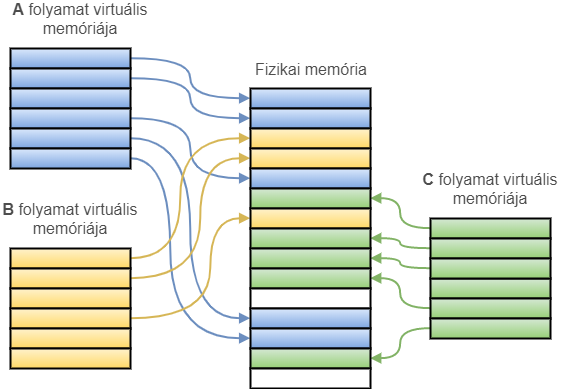
\includegraphics[width=0.6\textwidth]{img/paging.png}
        \caption{}
        \label{paging}
    \end{figure}

    \noindent A lapok mérete általában kettő hatványa ($2^k$).\\

    \paragraph*{Laptábla}

    \noindent A lapok és lapkeretek egymáshoz rendeléseit tartalmazza. Minden folyamatnak külön laptáblája van. A laptábla alapcím szerint indexelt, mezői üresek vagy a lapkeret címét tartalmazzák. Mezői tartalmazzák, hogy a laphoz tartozik-e lapkeret a fizikai memóriában, és ha van ilyen, akkor mi annak a címe. Hivatkozás esetén ez a lapcím keret a táblázatból a lapcím helyére másolódik. Ha nem tartozik hozzá lapkeret: laphiba kivétel történik és a kivételkezelő feladat a lapot valamelyik lapkeretbe elhelyezni. A laphiba kivétel mindig hiba (fault), azaz a végén a kivételt okozó utasítás a kivétel kezelése után újra végrehajtódik. A gyakori lapcím–lapkeret párokat egy gyorsítótárban tároljuk.

    \begin{figure}[H]
        \centering
        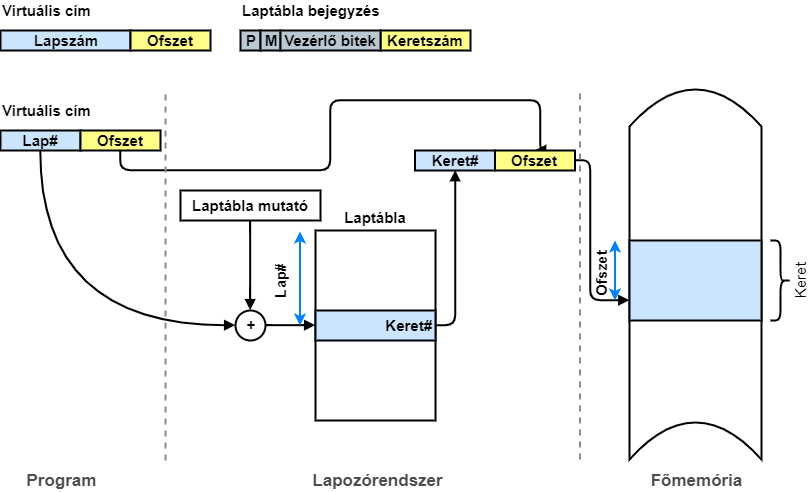
\includegraphics[width=0.9\textwidth]{img/paging_address_conversion.png}
        \caption{Címfordítás egy lapozó rendszerben}
        \label{paging_address_transformation}
    \end{figure}

    \paragraph*{A lapméret problematikája}

    \noindent Ha nagy a lapméretünk, akkor kicsit a laptábla, de belső elaprózódás lép fel (a kisebb folyamatok több memóriát kapnak, mint amire szükségük lenne).\\

    \noindent Ha kicsi a lapméret, akkor kevés memória veszik kárba, ellenben nagy a laptábla, ami viszont sok memóriát eszik. Erre megoldás a két szintű laptáblázat.

	\section*{Lapcserélési algoritmusok}
	
    Akkor válik szükségessé lapcsere, ha a használni kívánt programrész nincs a memóriában. Ezt az eseményt laphibának nevezik, ami kiváltja a lapcserélési eljárás megindítását.\\

   \noindent A hiányzó lapot be kell töltenünk vagy létre kell hoznunk egy üres lapot. Ha van üres lapkeret, ezt megtehetjük, ha nincs, akkor „ki kell dobnunk” egy lapot, a kérdés, hogy melyiket. Mivel a laphibakezelése sok erőforrást igényel, a cél a minél kevesebb laphiba.\\

   \noindent Fontos elemei a virtuális memóriakezelésnek a lapcserélési algoritmusok. Ezek többfélesége egyrészt a fejlődésüket, hatékonyabbá válásukat mutatja, másrészt esetleg ismerve a feladat milyenségét, egyikük valamilyen szempontból jobb lehet egy másiknál.

    \begin{itemize}[topsep=8pt,itemsep=4pt,partopsep=4pt, parsep=4pt]
        \item \textbf{Optimális} – egyben megvalósíthatatlan – \emph{lapcserélési algoritmus}. Ennek lényege, hogy a memóriában levő minden lapot megcímkézünk azzal a számmal, amelyik azt jelzi, hogy hány utasítás végrehajtása után kerül erre a lapra „sor”. Nyilván a legnagyobb számú lapot kellene kidobni, de az operációs rendszerek nem tudják megmondani a számot. Ehhez ugyanis először „virtuálisan” le kellene futtatni a programot, ami nyilvánvalóan abszurditás.

        \item \textbf{NRU} (Not Recently Used, nem mostanában használt) algoritmus:
        \begin{itemize}
            \item Minden laphoz, ami a memóriába kerül, hozzárendelünk még két bitet: egy R bitet, amely minden hivatkozáskor (akár olvasás, akár írás) egyesre állítódik, és egy M bitet, ami módosításkor kap 1-es értéket. Ennek alapján a memóriába lévő lapok négy osztályba sorolhatóak:
			\begin{itemize}
				\item 0.osztály: 00 (nem hivatkozott, nem módosított)
				\item 1.osztály: 01 (nem hivatkozott, módosított)
				\item 2.osztály: 10 (hivatkozott, nem módosított)
				\item 3.osztály: 11 (hivatkozott, módosított)
			\end{itemize}
			\item A módszer az, hogy véletlenszerűen kiválaszt a legalacsonyabb sorszámú osztályból egyet, és azt kidobja. Egyszerű módszer, könnyen megvalósítható.
		\end{itemize}
        \item \textbf{FIFO} (First-In First-Out) \emph{lapcserélési algoritmus}. A sor-adatszerkezet műveleteinek megfelelően lapcsere esetén a legrégebben bent lévő lapot eldobja, és a sor végére teszi az újonnan érkezőt.
        \item \textbf{Second chance} (második lehetőség) \emph{lapcserélési algoritmus}. A FIFO olyan módosítása, amelyben a legrégebbi egyes hivatkozású lapot nullás bittel a sor végére teszi, és keresi tovább a megfelelőt.
        \item \textbf{Az óra} \emph{lapcserélési algoritmus}: A bent lévő lapokat egy láncnak képzeljük, azaz nincs első és utolsó, eleje meg vége elem, hanem egy aktuális elem, amellyel utoljára volt dolgunk laphiba esetén. Innen indulva szintén az R bitet vizsgáljuk: amennyiben ez egyes, akkor nullára állítjuk, és megyünk tovább. Lényegében az előző algoritmus, csak a kitüntetett elem – ahonnan a keresés indul – az utolsónak hivatkozott változásra mutat.
		vizsgáljuk. Ha vizsgált lap hivatkozás bitje 0, akkor kitesszük.
        \item \textbf{LRU} (Least Recently Used) \emph{lapcserélési algoritmus}: Talán ez közelíti legjobban az optimális lapcserélést. Statisztikai megfontolásokra támaszkodik: az utoljára használt néhány utasítás által gyakran használt lap valószínűleg továbbra is szükséges lehet; viszont amit régen nem használtunk, valószínűleg még egy darabig nem is kell. Így azt dobjuk el, amelyiket a legrégebben nem használtunk. Az okozhat implementációs nehézséget, hogy minden hivatkozáskor aktualizálni kell a laphivatkozásokat. Ehhez minden lapbejegyzéshez felveszünk egy újabb bejegyzést, amely a lapra hivatkozáskor annak a számlálónak az értékét tartalmazza, amely minden memóriahivatkozás esetén eggyel nő.
        HW vagy SW megvalósítás.
        \begin{itemize}
            \item HW1: Vegyünk egy számlálót, ami minden memória hivatkozásnál 1-gyel nő. Minden laptáblában tudjuk ezt a számlálót tárolni. Minden memóriahivatkozásnál ezt a számlálót beírjuk a lapba. Laphibánál megkeressük a legkisebb számlálóértékű lapot.
            \item HW2: LRU bitmátrix használattal, n lap, n x n bitmátrix. Egy k. lapkeret hivatkozásnál állítsuk a mátrix k. sorát 1-re, míg a k. oszlopát 0-ra. Laphibánál a legkisebb értékű sor a legrégebbi.
		\end{itemize}
		\item \textbf{NFU} (Not Frequently Used) algoritmus:
		\begin{itemize}
            \item Minden laphoz tegyünk egy számlálót. Minden óramegszakításnál ehhez adjuk hozzá a lap hivatkozás (R) bitjét.
			\item Laphibánál a legkisebb számlálóértékű lapot dobjuk ki. (A leginkább nem használt lap)
			\item Hiba, hogy az NFU nem felejt, egy program elején gyakran használt lapok megőrzik nagy értéküket.
			\item Módosítsuk: Minden óramegszakításnál csináljunk jobbra egy biteltolást a számlálón, balról pedig hivatkozás bitet tegyük be (shr).(Öregítő algoritmus)
			\item Ez jól közelíti az \emph{LRU} algoritmust.
			\item Ez a lapszámláló véges bitszámú (n), így n időegység előtti eseményeket biztosan nem tud megkülönböztetni.
		\end{itemize}
	\end{itemize}

	\subsection*{Szegmentálás}

    A memóriát logikailag részekre un. szegmensekre osztják, és minden résznek megvan a saját, 0-tól kezdődő címtartománya. Egy memóriacím így két részből áll, egy szegmenscímből és egy eltolási- (offset) címből, azaz a memória kétdimenziós. Két szinten valósul meg, hardver és operációs rendszer szinten. A lapozással ellentétben ez nem marad rejtve a felhasználó (programozó) előtt.\\

    \noindent Szegmentálás nélkül egyetlen egydimenziós címterünk lenne, pl.:0-100 címig. Tegyük fel, hogy a programunk két folyamatosan növekvő méretű memóriaterületet használ. Előfordulhat, hogy az első a 0-49. címig tart, a második az 50-től 80-ig. Az első memóriaterületet nem tudjuk tovább növelni, pedig még lenne szabad memória a 81-től kezdődően. A megoldás a szegmentálás. Létrehozunk egy-egy szegmenst a két memóriaterület számára, mindkettő a 0. címtől kezdődik, így mindkét memóriaterületet addig tudjuk növelni amíg a memória el nem fogy.\\

    \begin{figure}[H]
        \centering
        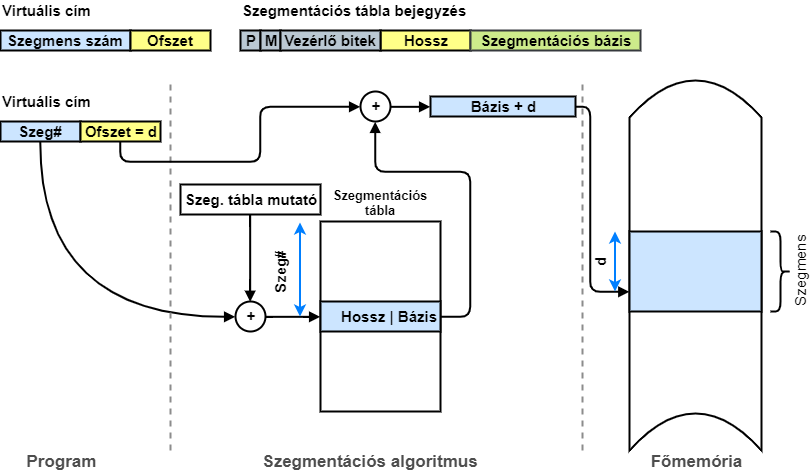
\includegraphics[width=0.9\textwidth]{img/segmentation_address_conversion.png}
        \caption{Címfordítás egy szegmentációval működő rendszerben}
        \label{segmentation_address_transformation}
    \end{figure}

    \noindent A szegmensekhez elérési jogok tartoznak:
    \begin{itemize}[topsep=8pt,itemsep=4pt,partopsep=4pt, parsep=4pt]
        \item írható,
        \item olvasható,
        \item futtatható.
    \end{itemize}

    \noindent Így például a programunk nem írhatja felül saját magát, mert a programkódot egy olyan szegmensben tároljuk, amely csak futtatható.\\

    \noindent A szegmentálás hasznos osztott programkönyvtárak használata esetén is. Ha a függvények külön-külön szegmensben helyezkednek el, akkor a programkönyvtár újabb verziójával a függvények kezdőcíme nem fog megváltozni, még akkor sem, ha a méretük megváltozik.\\

    \noindent Kétféleképp lehet megvalósítani:
    \begin{itemize}[topsep=8pt,itemsep=4pt,partopsep=4pt, parsep=4pt]
        \item cseréléssel
        \item lapozással.
    \end{itemize}

    \noindent Cserélésnél a rendszer a memóriában csak néhány szegmenst tárol. Kezdetben a szegmensek folyamatosan helyezkednek el. Ha a memória betelt, és egy olyan szegmensre van szükség, amely nincs benn a memóriában, helyet kell neki csinálni, azaz ki kell egyet írni a lemezre. Mivel egy szegmenst csak a vele legalább egyenlő méretű helyre tudunk beilleszteni, a memória előbb-utóbb lyukacsossá válik -mivel a pontos illeszkedés valószínűsége csekély- , ezt hívják külső elaprózódásnak. Ennek elkerülésére több módszer lehetséges. Az egyik, hogy a szegmenseket a memória eleje felé tolják, így a sok apró lyuk helyett a memória végén egy nagy lyuk keletkezik. Egy másik, hatékonyabb módszer, hogy olyan szegmenseket írnak ki a lemezre, amelyek két lyuk közé esnek, így a lyukak mérete nő.\\

    \noindent Lapozásnál nem teljes szegmensek cserélődnek, hanem ezeket a rendszer fix méretű részekre -lapokra- osztja. Ezeket a lapokat írja ki, vagy olvassa be. A klasszikus lapozáshoz képest, a különbség csak annyi, hogy minden szegmensnek külön laptábla kell.

	\section*{Lemezterület-szervezés, redundáns tömbök, fájlrendszerek szolgáltatásai és jellemző megvalósításaik}
	
    \subsubsection*{Partíciók}

    \begin{itemize}[topsep=8pt,itemsep=4pt,partopsep=4pt, parsep=4pt]
        \item A partícionálással a lemezt független szeletekre osztjuk.
        \item A partíciók az alkalmazások és az OS magasabb rétegei számára általában a lemezegységekhez hasonló eszközként látszanak.
        \item Az egyes partíciókat különböző célokra használhatjuk:
        \begin{itemize}
            \item Nyers partíciók (pl. adatbáziskezelőknek)
            \item Virtuális memóriaterület (swap)
            \item Fájlrendszer
        \end{itemize}
    \end{itemize}

	\subsection*{Redundáns tömbök}
	
    \textbf{RAID} -- Redundant Array of Inexpensive Disks. (olcsó lemezegységek redundáns tömbje)\\

    \noindent Szoftverből és hardverből is megvalósítható
    \begin{itemize}[topsep=8pt,itemsep=4pt,partopsep=4pt, parsep=4pt]
        \item Hardver-RAID esetén általában egész diszkeket kötünk össze egy külső vezérlőegységgel, az OS szemszögéből az eredmény egy szokásos lemezegységnek látszik (RAID diszkrendszer)
        \item Szoftver-RAID-et az OS valósítja meg, így partíciók felett is működhet
        \item A hardver megvalósítás drágább, de hatékonyabb
    \end{itemize}

    \noindent Bár nevében szerepel az olcsó (Inexpensive), valójában inkább nem az. Több lemezt fog össze, és egy logikai egységként látja az operációs rendszer.\\
    Többféle ,,összefogási" elv létezik: RAID 0-6 (7).\\

	\paragraph*{RAID 0 (összefűzés vagy síkozás)}

    \begin{itemize}[topsep=8pt,itemsep=4pt,partopsep=4pt, parsep=4pt]
        \item Néhány diszk tárterületének összefűzésével megsokszorozhatjuk az összefüggő(nek látszó) tárkapacitást
        \item A logikai diszk blokkjait általában felváltva osztjuk szét a fizikai diszkek szektorai között (striping)
        \item Az IO műveletek párhuzamosításával nő a teljesítmény
        \item Nincs redundancia
        \item Nő az adatvesztés esélye
        \item Általában a blokknál nagyobb egységeket kezelünk (stripe), de akár bitszintű szétosztás is lehetséges
    \end{itemize}

    \begin{figure}[H]
        \centering
        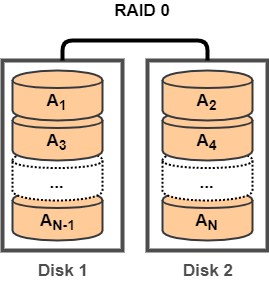
\includegraphics[width=0.325\textwidth]{img/raid0.png}
        \caption{RAID 0}
        \label{ref:raid0}
    \end{figure}

    {\footnotesize \noindent {\color{blue} \faLightbulbO\ $\triangleright$ } }
    {\footnotesize
    \noindent A RAID 0 az egyes lemezek egyszerű összefűzését jelenti, viszont semmilyen redundanciát nem ad, így nem biztosít hibatűrést, azaz egyetlen meghajtó meghibásodása az egész tömb hibáját okozza. Mind az írási, mind az olvasási műveletek párhuzamosítva történnek, ideális esetben a sebesség az egyes lemezek sebességének összege lesz, így a módszer a RAID szintek közül a legjobb teljesítményt nyújtja. A megoldás lehetővé teszi különböző kapacitású lemezek összekapcsolását is, viszont a nagyobb kapacitású lemezeken is csak a tömb legkisebb kapacitású lemezének méretét lehet használni.
    $\triangleleft$ \faLightbulbO}\\

    \noindent A RAID 0 főleg olyan helyeken alkalmazható, ahol nem szempont az adatbiztonság vagy kevés merevlemez csatolható fel az operációs rendszer korlátozása miatt. A másik pozitív tulajdonsága viszont továbbra is csábító lehet olyan, kifejezetten csak játékra épített rendszereknél, ahol ezzel tetemes teljesítménynövekedést érhetünk el. Ilyen célú alkalmazásra mégsem túl ajánlott, mivel az egyszer már összekapcsolt diszkek különálló alkalmazása csak újraszervezés után, a teljes adattartalom eltávolításával és újraformázással lehetséges.\\

    \noindent A RAID 0 legfontosabb paraméterei
    \begin{itemize}[topsep=8pt,itemsep=4pt,partopsep=4pt, parsep=4pt]
        \item olvasás: nincs overhead (elemszám * olvasási sebesség)
        \item írás: nincs overhead (elemszám * írási sebesség)
        \item tárolókapacitás: egyenesen arányos (elemszám * tárolókapacitás)
        \item meghibásodási tolerancia: nincs
    \end{itemize}

	\paragraph*{RAID 1 (tükrözés)}

    \begin{itemize}[topsep=8pt,itemsep=4pt,partopsep=4pt, parsep=4pt]
        \item Minden adatot két független diszken tárolunk
        \item A tárolókapacitás a felére csökken
        \item Olvasási teljesítmény nőhet, írás nem változik, vagy kissé csökken
        \item Diszkhibából eredő adatvesztés esélye jelentősen csökken
        \item Egyszerű, de drága megoldás
        \item Nagyon kicsi processzorigény
        \item 1 GB adat tárolásához 2 GB diszkterület szükséges
    \end{itemize}

    \begin{figure}[H]
        \centering
        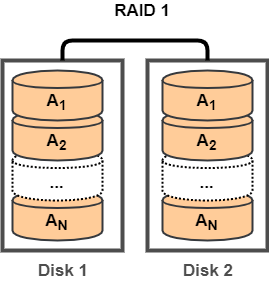
\includegraphics[width=0.325\textwidth]{img/raid1.png}
        \caption{RAID 1}
        \label{ref:raid1}
    \end{figure}

    {\footnotesize \noindent {\color{blue} \faLightbulbO\ $\triangleright$ } }
    {\footnotesize
    \noindent A RAID 1 eljárás alapja az adatok tükrözése (disk mirroring), azaz az információk egyidejű tárolása a tömb minden elemén. A kapott logikai lemez a tömb legkisebb elemével lesz egyenlő méretű. Az adatok olvasása párhuzamosan történik a diszkekről, felgyorsítva az olvasás sebességét; az írás normál sebességgel, párhuzamosan történik a meghajtókon. Az eljárás igen jó hibavédelmet biztosít, bármely meghajtó meghibásodása esetén folytatódhat a működés. A RAID 1 önmagában nem használja a csíkokra bontás módszerét.

    \noindent A RAID 1 legfontosabb paraméterei
    \begin{itemize}[topsep=8pt,itemsep=4pt,partopsep=4pt, parsep=4pt]
        \item olvasás: nincs overhead (elemszám * olvasási sebesség)
        \item írás: overhead - a tükrözés kétszer annyi írási művelettel jár (elemszám * írási sebesség / 2)
        \item tárolókapacitás: a tükrözött elemek fele (elemszám * tárolókapacitás / 2)
        \item meghibásodási tolerancia: (elemek száma - 1) elem
    \end{itemize}
    $\triangleleft$ \faLightbulbO}\\

	\paragraph*{RAID 2 (ECC)}

    \begin{itemize}[topsep=8pt,itemsep=4pt,partopsep=4pt, parsep=4pt]
        \item A gépi memóriánál megszokott hibajavító kódok használata (ECC memória)
        \item Az adatbitek mellett néhány extra bitet is tárolunk (lásd Hamming kódok)
        \item A bájt bitjeit és a hibajavító biteket tároljuk különböző diszkeken
        \item Az egyik diszk meghibásodása esetén a paritásbitekből helyreállítható a hiányzó bit
        \item pl. 4 diszk kapacitáshoz elég 7 fizikai diszk
        \item A gyakorlatban ritkán használt
    \end{itemize}

    \begin{figure}[H]
        \centering
        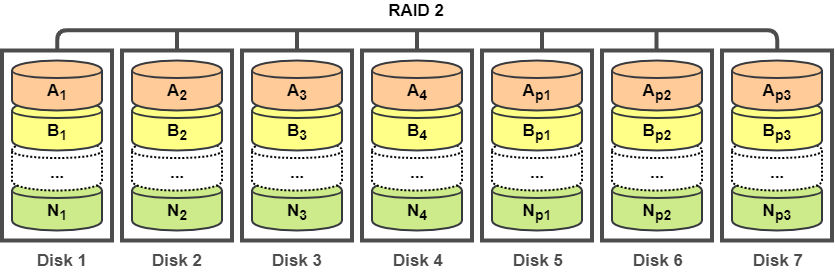
\includegraphics[width=0.9\textwidth]{img/raid2.png}
        \caption{RAID 2}
        \label{ref:raid2}
    \end{figure}

    {\footnotesize \noindent {\color{blue} \faLightbulbO\ $\triangleright$ } }
    {\footnotesize
    \noindent A RAID 2 használja a csíkokra bontás módszerét, emellett egyes meghajtókat hibajavító kód (ECC: Error Correcting Code) tárolására tartanak fenn. A hibajavító kód lényege, hogy az adatbitekből valamilyen matematikai művelet segítségével redundáns biteket képeznek. A használt eljárástól függően a kapott kód akár több bithiba észlelésére, illetve javítására (ez utóbbi persze több redundanciát igényel) alkalmas. A védelem ára a megnövekedett adatmennyiség. Ezen meghajtók egy-egy csíkjában a különböző lemezeken azonos pozícióban elhelyezkedő csíkokból képzett hibajavító kódot tárolnak. A módszer esetleges lemezhiba esetén képes annak detektálására, illetve kijavítására. Manapság nem használják, mivel a SCSI meghajtókban már minden egyes szektorban az adott szektorhoz tartozó ECC is eltárolódik.
    $\triangleleft$ \faLightbulbO}\\

	\paragraph*{RAID 3 (paritásbitek)}

    \begin{itemize}[topsep=8pt,itemsep=4pt,partopsep=4pt, parsep=4pt]
        \item A memóriával ellentétben a P lemezegységek jelzik, ha hiba történik
        \item Nincs szükség a teljes hibajavító kódra, elég egyszerűen a paritásbitet tárolni (XOR)
        \item Az ismert pozíciójú hibás bit ebből helyreállítható
        \item Előnyök:
        \begin{itemize}
            \item Olcsó: n diszk kapacitáshoz elég n+1 diszk
            \item Egy blokk írása/olvasása szétosztódik a diszkek között, tehát felgyorsul
        \end{itemize}
        \item Hátrányok:
        \begin{itemize}
            \item Magasabb CPU igény
            \item I/O műveletekben az összes diszk részt vesz, a párhuzamos teljesítmény romlik
        \end{itemize}
    \end{itemize}

    \begin{figure}[H]
        \centering
        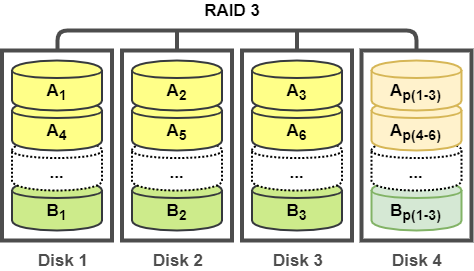
\includegraphics[width=0.65\textwidth]{img/raid3.png}
        \caption{RAID 3}
        \label{ref:raid3}
    \end{figure}

    {\footnotesize \noindent {\color{blue} \faLightbulbO\ $\triangleright$ } }
    {\footnotesize
    \noindent A RAID 3 felépítése hasonlít a RAID 2-re, viszont nem a teljes hibajavító kód, hanem csak egy lemeznyi paritásinformáció tárolódik. Egy adott paritáscsík a különböző lemezeken azonos pozícióban elhelyezkedő csíkokból XOR művelet segítségével kapható meg. A rendszerben egy meghajtó kiesése nem okoz problémát, mivel a rajta lévő információ a többi meghajtó (a paritást tároló meghajtót is beleértve) XOR-aként megkapható. Az alapvető különbség a RAID 2-ben alkalmazott hibajavító kóddal szemben, hogy itt feltesszük, hogy a meghajtó meghibásodását valamilyen módon (például többszöri sikertelen olvasás hatására) észleljük, majd a meghibásodott diszken lévő információt a többi diszken lévő adatok segítségével állítjuk elő. A RAID 2 a diszkhibák ellen is védelmet nyújt, például egyes bájtok megsérülése esetén. (Vegyük észre, hogy csak az XOR-os paritásbit technikát használva az egyik meghajtón egy adott bájt megsérülése esetén csak azt vennénk észre, hogy a különböző meghajtókon az azonos csíkba tartozó részek XOR-a nem nullát adna, de nem tudnánk sem azt, hogy melyik meghajtón van a hiba, sem azt, hogy hogyan javítsuk ki. Ezért van szükség a szektoronkénti hibajavító kód alkalmazására.)

    \noindent A RAID 3-nál kisméretű csíkokat definiálnak, így az egyes fájlok olvasása és írása párhuzamosan történhet az egyes meghajtókon, viszont a módszer nem támogatja egyszerre több kérés párhuzamos kiszolgálását (single-user mode). (Természetesen a paritáscsíkot minden egyes íráskor módosítani kell, amihez szükséges a korábbi tartalom kiolvasása. Viszont például fájltranszfer esetén, pont a kisméretű csíkok miatt, az azonos pozícióban lévő csíkokat általában az összes diszken felülírják, így ez esetben a probléma kevésbé jelentkezik.)
    $\triangleleft$ \faLightbulbO}\\

	\paragraph*{RAID 4 (paritásblokkok)}

    \begin{itemize}[topsep=8pt,itemsep=4pt,partopsep=4pt, parsep=4pt]
        \item  A RAID 0 megoldást egészítsük ki egy P paritásdiszkkel
        \item Nincs szükség a bájtok felszabdalására, a paritás független blokkokra is számolható
        \item Egy diszk kiesése esetén a paritásdiszk és a többi diszk blokkjaiból helyreállíthatók az adatok
        \item Előnyök:
        \begin{itemize}
            \item A RAID 3-hoz hasonlóan olcsó
            \item Egy blokk beolvasásához elég egyetlen diszk, így a független olvasások párhuzamosíthatók
        \end{itemize}
        \item Hátrányok:
        \begin{itemize}
            \item Az egyedi olvasásműveletek sebessége csökken
            \item Az írások nem párhuzamosíthatóak (a paritásdiszket minden írás használja)
            \item A diszkek igénybevétele nem egyforma
        \end{itemize}
    \end{itemize}

    \begin{figure}[H]
        \centering
        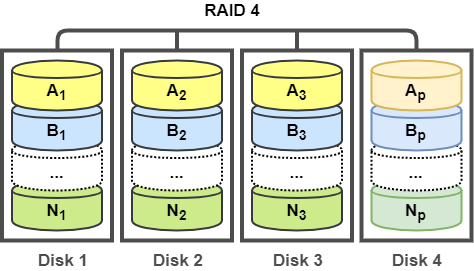
\includegraphics[width=0.65\textwidth]{img/raid4.png}
        \caption{RAID 4}
        \label{ref:raid4}
    \end{figure}

    {\footnotesize \noindent {\color{blue} \faLightbulbO\ $\triangleright$ } }
    {\footnotesize
    \noindent A RAID 4 felépítése a RAID 3-mal megegyezik. Az egyetlen különbség, hogy itt nagyméretű csíkokat definiálnak, így egy rekord egy meghajtón helyezkedik el, lehetővé téve egyszerre több (különböző meghajtókon elhelyezkedő) rekord párhuzamos írását, illetve olvasását (multi-user mode). Problémát okoz viszont, hogy a paritás-meghajtó adott csíkját minden egyes íráskor frissíteni kell (plusz egy olvasás és írás), aminek következtében párhuzamos íráskor a paritásmeghajtó a rendszer szűk keresztmetszetévé válik. Ezenkívül valamely meghajtó kiesése esetén a rendszer olvasási teljesítménye is lecsökken, a paritás-meghajtó jelentette szűk keresztmetszet miatt.
    $\triangleleft$ \faLightbulbO}\\

    \noindent Ma ezen megoldások (RAID 2,3,4) nem gyakran használatosak.\\
\newpage
	\paragraph*{RAID 5 (elosztott paritásblokkok)}

    \begin{itemize}[topsep=8pt,itemsep=4pt,partopsep=4pt, parsep=4pt]
        \item A RAID 4 javítása: a paritásblokkokat keverjük az adatblokkok közé
        \item Például egy 5 diszkből álló tömbben az n. blokkhoz tartozó paritásblokkot tároljuk az (n mod 5)+1. diszken, a többi diszk n. blokkjai tárolják az adatokat
        \item A diszkek igénybevétele kiegyenlítődik
        \item Az írások némileg párhuzamosíthatók, azonban még mindig jóval lassabbak az egyszerű tükrözésnél
    \end{itemize}

    \begin{figure}[H]
        \centering
        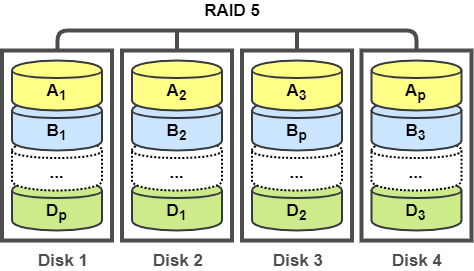
\includegraphics[width=0.65\textwidth]{img/raid5.png}
        \caption{RAID 5}
        \label{ref:raid5}
    \end{figure}

    {\footnotesize \noindent {\color{blue} \faLightbulbO\ $\triangleright$ } }
    {\footnotesize
    \noindent A RAID 5 a paritás információt nem egy kitüntetett meghajtón, hanem „körbeforgó paritás” (rotating parity) használatával, egyenletesen az összes meghajtón elosztva tárolja, kiküszöbölve a paritás-meghajtó jelentette szűk keresztmetszetet. Minimális meghajtószám: 3, de az írási sebesség csökkenésének elkerülése érdekében 4 elemnél kevesebb nem ajánlott. Mind az írási, mind az olvasási műveletek párhuzamosan végezhetőek. Egy meghajtó meghibásodása esetén az adatok sértetlenül visszaolvashatóak, a hibás meghajtó adatait a vezérlő a többi meghajtóról ki tudja számolni. A csíkméret változtatható; kis méretű csíkok esetén a RAID 3-hoz hasonló működést, míg nagy méretű csíkok alkalmazása esetén a RAID 4-hez hasonló működést kapunk. A hibás meghajtót ajánlott azonnal cserélni, mert két meghajtó meghibásodása esetén az adatok elvesznek!\\

    \noindent Az írási sebességnél fontos figyelembe venni a paritás adatok előállítására szükséges számítási kapacitás igényt! Szoftveres megoldásnál ez jelentős processzorterhelést, illetve az írási sebesség csökkenését eredményezheti, ezért ajánlott a hardveres megoldás, ahol a célhardver látja el ezeket a feladatokat.\\

    \noindent A RAID 5 vezérlők a hibás meghajtó helyére betett új, üres meghajtót automatikusan fel tudják tölteni az eredeti adatokkal.\\

    \noindent A hibás meghajtó egy-egy blokkját a következőképpen lehet visszaolvasni: Ah=(Aj1 XOR Aj2) XOR Aj3, ahol Ah: a fizikailag hibás meghajtó része és Aj1, Aj2, Aj3: a jó meghajtó része.\\

    \noindent A tömb egyetlen meghajtójáról nem állítható vissza a teljes adattartalom, viszont egy-egy adatblokknyi igen. Mivel akár ez is tartalmazhat értékes információt, így a már nem használt vagy hibás adathordozót érdemes megsemmisíttetni.\\\\

    \noindent A RAID 5 legfontosabb paraméterei
    \begin{itemize}[topsep=8pt,itemsep=4pt,partopsep=4pt, parsep=4pt]
        \item olvasás: nincs overhead (elemszám * olvasási sebesség)
        \item írás: jelentős overhead
        \begin{enumerate}
            \item adat olvasása,
            \item paritás olvasása,
            \item adat írása,
            \item paritás írása
        \end{enumerate}
        (elemszám * írási sebesség / 4)
        \item tárolókapacitás: az elosztott paritás miatt kiesik 1 elem (elemszám-1 * tárolókapacitás)
        \item meghibásodási tolerancia: 1 elem
    \end{itemize}
    $\triangleleft$ \faLightbulbO}\\

    \paragraph*{RAID 6 (P+Q)}

    \begin{itemize}[topsep=8pt,itemsep=4pt,partopsep=4pt, parsep=4pt]
        \item Paritásblokk (P) mellett hibajavító kódok (Q, Reed-Solomon)
        \item n+2 diszk költséggel n diszknyi kapacitást nyújt, és bármely két diszk kiesését elviseli
        \item Matematikai háttér: Galois-terek
        \item Jelentős, a RAID 5-nél is magasabb CPU igény
        \item Elvileg általánosítható kettőnél több diszk kiesésére, a gyakorlatban általában nem éri meg
        \item A P és Q blokkokat célszerű itt is az adatblokkok közé keverni
    \end{itemize}

    \begin{figure}[H]
        \centering
        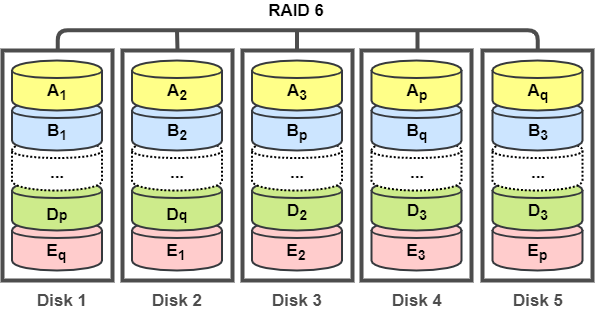
\includegraphics[width=0.65\textwidth]{img/raid6.png}
        \caption{RAID 6}
        \label{ref:raid6}
    \end{figure}

    {\footnotesize \noindent {\color{blue} \faLightbulbO\ $\triangleright$ } }
    {\footnotesize
    \noindent A RAID 6 tekinthető a RAID 5 kibővítésének. Itt nemcsak soronként, hanem oszloponként is kiszámítják a paritást. A módszer segítségével kétszeres meghajtómeghibásodás is kiküszöbölhetővé válik. A paritáscsíkokat itt is az egyes meghajtók között, egyenletesen elosztva tárolják, de ezek természetesen kétszer annyi helyet foglalnak el, mint a RAID 5 esetében, valamint még nagyobb az írási műveletek overheadje. Ennek ellenére, nagy elemszám esetén a RAID 6 lényegesen biztonságosabb alternatívája a RAID 5-nek, valamint arányaiban kevesebb tárkapacitás veszteséggel jár.\\

    \noindent Egy RAID 6 tömb legalább 4 elemből kell álljon, de az írási sebesség csökkenésének elkerülése érdekében 6 elemnél kevesebb nem ajánlott.\\\\

    \noindent A RAID 6 legfontosabb paraméterei
    \begin{itemize}[topsep=8pt,itemsep=4pt,partopsep=4pt, parsep=4pt]
        \item olvasás: nincs overhead (elemszám * olvasási sebesség)
        \item írás: jelentős overhead
        \begin{enumerate}
            \item adat olvasása,
            \item vízszintes paritás olvasása,
            \item függőleges paritás olvasása,
            \item adat írása,
            \item vízszintes paritás írása,
            \item függőleges paritás írása,
        \end{enumerate}
        (elemszám * írási sebesség / 6)
        \item tárolókapacitás: a kétféle elosztott paritás miatt kiesik 2 elem (elemszám-2 * tárolókapacitás)
        \item meghibásodási tolerancia: 2 elem
    \end{itemize}
    $\triangleleft$ \faLightbulbO}\\

	\paragraph*{RAID 1+0 (RAID 10)}

    {\footnotesize \noindent {\color{blue} \faLightbulbO\ $\triangleright$ } }
    {\footnotesize
    \noindent Hasonlít a RAID 01 megoldáshoz, annyi különbséggel, hogy itt a lemezeket először tükrözzük, majd a kapott tömböket fűzzük össze. Ez biztonság szempontjából jobb megoldás, mint a RAID 01, mivel egy diszk kiesése csak az adott tükrözött tömböt érinti, a rá épült RAID 0-t nem; sebességben pedig megegyezik vele.\\

    \noindent Hátránya, hogy legalább 4 adathordozóra van szükség, ahol 1-1 tükrözött adathordozó kerül összefűzésre, ezért az egyes adathordozók összes tárkapacitásának mindössze a fele felhasználható a tömbben. Előnye azonban az összefűzésből fakadó írási sebesség növekedés, valamint egy sajátos, több elemre is kiterjedő redundancia.\\\\

    \noindent A RAID 10 legfontosabb paraméterei
    \begin{itemize}[topsep=8pt,itemsep=4pt,partopsep=4pt, parsep=4pt]
        \item olvasás: nincs overhead (elemszám * olvasási sebesség)
        \item írás: overhead - a tükrözés kétszer annyi írási művelettel jár (elemszám * írási sebesség / 2)
        \item tárolókapacitás: a tükrözött elemek fele (elemszám * tárolókapacitás / 2)
        \item meghibásodási tolerancia: legalább 1 elem, de legfeljebb a tömb elemszámának fele (amennyiben kizárólag független kettőzött elemek hibásodnak meg)
    \end{itemize}
    }

    \begin{figure}[H]
        \centering
        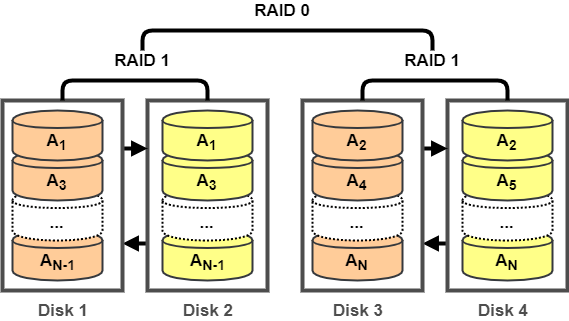
\includegraphics[width=0.65\textwidth]{img/raid1+0.png}
        \caption{RAID 1+0}
        \label{ref:raid10}
    \end{figure}

	\paragraph*{RAID 0+1 (RAID 01)}

    \noindent Ez egy olyan hibrid megoldás, amelyben a RAID 0 által hordozott sebességet a RAID 1-et jellemző biztonsággal ötvözhetjük. Hátránya, hogy minimálisan 4 eszközre van szükségünk, melyekből 1-1-et összefűzve, majd páronként tükrözve építhetjük fel a tömbünket, ezért a teljes kinyerhető kapacitásnak mindössze a felét tudjuk használni. Mivel a tükrözés (RAID 1) a két összefűzött (RAID 0) tömbre épül, ezért egy lemez meghibásodása esetén az egyik összefűzött tömb mindenképp kiesik, így a tükrözés is megszűnik. Fontos megjegyeznünk, hogy ez a megoldás legalább négy darab merevlemezt igényel.

    \begin{figure}[H]
        \centering
        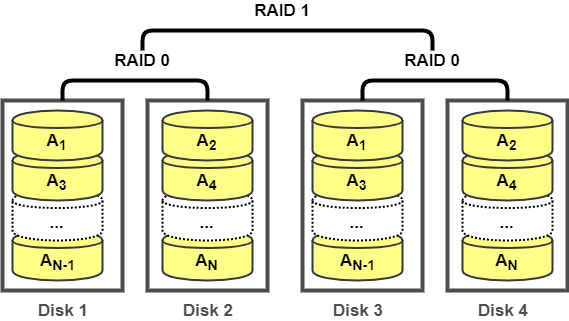
\includegraphics[width=0.65\textwidth]{img/raid0+1.png}
        \caption{RAID 0+1}
        \label{ref:raid01}
    \end{figure}
	
    \noindent A vezérlők gyakran nyújtják egyiket, másikat, mivel így is, úgy is tükrözés van, azaz drága, így ritkán használt.\\

    \paragraph*{RAID összefoglalás\\}

    \begin{itemize}[topsep=8pt,itemsep=4pt,partopsep=4pt, parsep=4pt]
        \item A gyakorlatban csak a 0., 1., 5. és 6. szinteket alkalmazzák, illetve az 1+0, 0+1 kombinált megoldásokat
        \item A komponens diszkek méretének egyformának kell lennie
        \item Új diszkek menet közbeni hozzáadásával nem lehet növelni a tárkapacitást, újra létre kell hozni a tömböt
        \item A 6. illetve szerencsés esetben az 1+0, 0+1 kivételével valamennyi szint csak egyetlen diszk kiesését viseli el
        \item Választási szempontok:
        \begin{itemize}
            \item Magas megbízhatóság: 1, 5, 6, 1+0, 0+1
            \item Nagy teljesítmény: 0, 1, 1+0, 0+1
            \item Alacsony költség: 0, 5, 6
            \item Ezek közül bármelyik kettőt teljesíthetjük
        \end{itemize}
        \item Minden rendszernél külön kell mérlegelni, melyik a legmegfelelőbb megoldás; gyakran több különböző RAID szintű és méretű tömböt definiálunk
        \item Általában lehetőség van készenléti diszkek definiálására, melyeket a rendszer automatikusan üzembe állít, ha egy diszk kiesik
        \begin{itemize}
            \item Az új diszk szinkronizációja időbe telik, ezalatt a tömb teljesítménye csökken
            \item A szinkronizáció közbeni új diszkhiba végzetes (a RAID-6 ez ellen védelmet nyújt)
        \end{itemize}
        \item A redundáns tömbök nem nyújtanak védelmet minden hibalehetőség ellen
        \begin{itemize}
          \item Emberi tévedések
          \item Programhibák
          \item Az egész rendszert érintő hibák
        \end{itemize}
        \item Váratlan leállások
        \item Túlfeszültség
        \item Természeti katasztrófák
        \item A fejlett operációs rendszerek kötetkezelő rendszerekkel (volume manager) könnyítik meg a hibatűrő logikai diszkek létrehozását és üzemeltetését
        \begin{itemize}
            \item Új indirekciós szint a logikai blokkok és a RAID tömbök fizikai blokkjai között
            \item A kötetkezelő rendszertől a partíciókhoz hasonló, de rugalmasan átméretezhető, \\
            hibatűrő logikai tárterületek (kötetek) igényelhetők
            \item A rábízott fizikai partíciók tárterületével a kötetkezelő automatikusan gazdálkodik
        \end{itemize}
    \end{itemize}
	
	\subsection*{Fájlrendszerek szolgáltatásai}
	
    \noindent Az adatállományok a rendelkezésre álló lemezterületen történő tárolásának és elrendezésének módszere a fájlrendszer.\\

    \noindent \textbf{Fájl}\\

    \noindent Olyan bitsorozat, melyek tartalma a folyamat befejeződése vagy a rendszer újraindítása után sem veszik el. \\
	\noindent A fájlok logikai szerkezete lehet

	\begin{itemize}[topsep=8pt,itemsep=4pt,partopsep=4pt, parsep=4pt]
		\item bájtsorozat
		\item fix méretű rekordok sorozata
		\item változó méretű rekordok sorozata (szövegsorok)
        \item egyéb (például szegmensekre osztott programfájlok stb.)
	\end{itemize}

    \noindent Fizikai szerkezetét tekintve egy blokksorozat, amely nem feltétlenül egymást követő blokkokból áll (töredezés). És az utolsó blokkja általában töredékblokk (nem tölti ki feltétlenül a teljes blokkot).

    \noindent A fájl az információtartalmán túl a fájlt leíró ún. meta-adatokat vagy attribútumokat is tárolunk:
    \begin{itemize}[topsep=8pt,itemsep=4pt,partopsep=4pt, parsep=4pt]
      \item neve
      \item elhelyezkedése a lemezen
      \item mérete
      \item tulajdonosai, elérési jogosultságok
      \item elérési és egyéb időbélyegek
      \item $\ldots$
    \end{itemize}

    \noindent A meta-adatokat a fájl tartalmától elkülönítve önálló fájlleíró blokkokban tároljuk a lemezen.\\

    \noindent A fájl típusa közli, hogy a fájl tartalma hogyan értelmezhető
    \begin{itemize}
      \item Expilict meta-attributumokban (pl MAC)
      \item A fájlnévbe építve, kiterjesztés formájában (Windows)
      \item A fájl tartalmában elhelyezett speciális kódokkal (UNIX)
    \end{itemize}

    \noindent A fájl műveletei
    \begin{itemize}[topsep=8pt,itemsep=4pt,partopsep=4pt, parsep=4pt]
        \item Új, üres fájl létrehozása
        \item Egy létező fájl törlése
        \item Írás (felülírás, beszúrás, hozzáfűzés)
        \item Olvasás (szekvenciális vagy közvetlen)
        \item Újrapozíciónálás (szekvenciális írás/olvasás)
        \item Meta-adatok lekérdezése, módosítása (például: Átnevezés)
        \item Zárolás
        \item $\ldots$
    \end{itemize}

    \noindent A fájlrendszer feladata a fenti műveletek hatékony implementációja.\\

    \noindent A könyvtár a fájlrendszerben tárolt fájlokról tárolt jegyzék. Egy könyvtár alá tartozhatnak további könyvtárak ún. alkönyvtárak (egymásba ágyazás). Ez esetben minden könyvtárnak pontosan egy szülője lehet, kivéve a gyökér könyvtár, aminek nincs szülője. A könyvtárak hierarchiája fa szerkezetű.\\

    \noindent Egy fájl útvonala a gyökérkönyvtár a fájlt tartalmazó könyvtárral összekötő út a könyvtárszerkezetben.\\

    \noindent A rendszer a folyamatokhoz aktuális könyvtárat rendel. Ehhez az aktuális könyvtárhoz képest egy fájl vagy könyvtár hivatkozható relatív elérési úttal is.\\

    \noindent A könyvtáraknak is vannak meta-adatai:
    \begin{itemize}[topsep=8pt,itemsep=4pt,partopsep=4pt, parsep=4pt]
        \item neve,
        \item tulajdonos, elérési jogosultságok
        \item időbélyegzők
    \end{itemize}

    \noindent A könyvtár műveletei:
    \begin{itemize}[topsep=8pt,itemsep=4pt,partopsep=4pt, parsep=4pt]
        \item Új, üres könyvtár létrehozása
        \item Egy létező könyvtár törlése
        \item Listázás
        \item Bejárás
        \item Keresés
        \item Meta-adatok lekérdezése, módosítása (például: Átnevezés)
        \item $\ldots$
    \end{itemize}

    \noindent A fájlkezelés alrendszerét rétegekre oszthatjuk. Az egyes rétegek csak a közvetlenül alattuk és fölöttük lévő rétegekkel kommunikálnak. Az alsó réteg szolgáltatásait használják, és a felső réteg számára szolgáltatásokat nyújtanak.

	\begin{figure}[H]
		\centering
		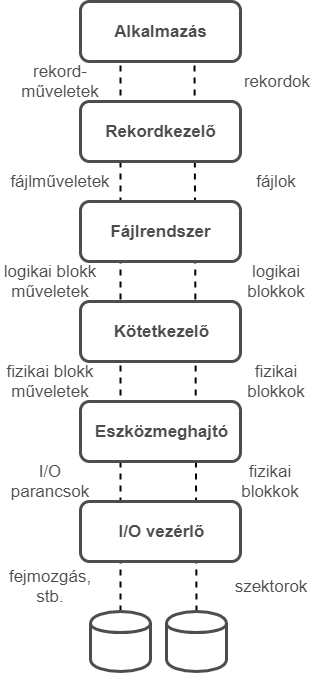
\includegraphics[width=0.4\textwidth]{img/file_system_management.png}
		\caption{Fájl-kezelés}
        \label{file_system_management}
	\end{figure}

	\noindent Fájlrendszer típusok:
	\begin{itemize}[topsep=8pt,itemsep=4pt,partopsep=4pt, parsep=4pt]
		\item Merevlemezen alkalmazott fájlrendszer: FAT, NTFS, EXT2FS, XFS, stb
		\item Szalagos rendszereken (elsősorban backup) alkalmazott fájlrendszer: Tartalomjegyzék, majd a tartalom szekvenciálisan
		\item CD, DVD, Magneto-opto Disc fájlrendszer: CDFS, UDF (Universal Disc Format)
		\item RAM lemezek (ma már kevésbé használtak)
		\item FLASH memória meghajtó (FAT32)
		\item Hálózati meghajtó: NFS
		\item Egyéb pszeudó fájlrendszerek: Zip, tar.gz, ISO
	\end{itemize}

    \noindent A kezdeti UNIX és UNIX-szerű operációs rendszerek (így pl. a GNU/LINUX operációs rendszer is) csak egyfajta fájlrendszert támogattak, a saját formátumukat. A modern operációs rendszerek viszont többféle fájlrendszert is támogatnak, és vannak olyan fájlrendszerek is, amelyeket több operációs rendszer is támogat.

	\subsection*{Fájlrendszerek szolgáltatásainak jellemző megvalósításai\\}
	
    \paragraph*{A lemezen tárolt adatszerkezetek\\}

    \begin{itemize}[topsep=8pt,itemsep=4pt,partopsep=4pt, parsep=4pt]
        \item Boot blokk
        \item Fájlrendszer-leíró blokk vagy blokkok (superblock)
        \begin{itemize}[topsep=8pt,itemsep=4pt,partopsep=4pt, parsep=4pt]
            \item Fájlok száma
            \item Blokkok száma és mérete
            \item Szabad blokkok száma
            \item A fájlrendszer állapota (tiszta, gyanús, hibás)
            \item Időbélyegzők
            \begin{itemize}
                \item Utolsó csatolás
                \item Utolsó ellenőrzés
                \item Utolsó modosítás
            \end{itemize}
            \item Fájlrendszer címkéje
        \end{itemize}
        \item Könyvtárszerezet a fájlok szervezéséhez
        \item Fájlleíró blokkok (i-node) a fájlok metaadatainak tárolására
    \end{itemize}

    \noindent Superblock nélkül a fájlrendszer nem használható, ezért több példányban is eltárolják általában.

    \paragraph*{A memóriában tárolt adatszerkezetek\\}
    \begin{itemize}[topsep=8pt,itemsep=4pt,partopsep=4pt, parsep=4pt]
      \item Csatolt fájlrendszerek táblázata
      \item Nemrégiben használt könyvtárak táblázata
      \item Rendszerben megnyitott összes fájl leírása
      \item Folyamatonkénti táblázat a folyamat megnyitott fájlairól
      \item Blokk gyorsítótár
    \end{itemize}

    \noindent A könyvtárakat általában speciális tartalmú adatállományokkal reprezentálják. Hasonló a fájlok tárolásához.\\

    \subsection*{Blokkfoglalás}

    \noindent A fájlok tartalmát adatblokkokban tárolja
    \begin{itemize}[topsep=8pt,itemsep=4pt,partopsep=4pt, parsep=4pt]
      \item Nyilvántartja mely blokkok tartoznak egy fájlhoz és milyen sorrendben
      \item Tudnia kell egy új blokkok hozzáadását egy már létező fájlhoz
    \end{itemize}

    \noindent A blokkok nyilvántartását metaadatok között tárolja magában az i-node-ban, vagy a lemez egy erre a célra elkülönített területén.

    \paragraph*{Folytonos blokkfoglalás}

    Legyenek a fájlok blokkjai együtt egy folytonos lemezterületen
    \begin{itemize}[topsep=8pt,itemsep=4pt,partopsep=4pt, parsep=4pt]
      \item Dinamikus partíciók használhatók
      \item Egy fájl blokkjainak nyilvántartásához elég a kezdőblokkot és a fájl hosszát tárolni.
      \item Nagyon hatékony, mivel kizárja a fájl töredezettségéből eredő fejmozgásokat
      \item \emph{Hátrányai:}
      \begin{itemize}
        \item A szabad terület elaprozódása miatt külső töredezettség
        \item Mivel a végső fájlméretet előre meg kell adni, a lassan növő fájlok jelentős belső töredezettséget eredményeznek
        \item A fájlméret utólag nehezen növelhető
      \end{itemize}
      \item Csak olvasható háttértárakon (CD, DVD, stb.), illetve nagy I/O teljesítmény esetén (nagyszámítógépek) éri meg használni
    \end{itemize}

    \paragraph*{Láncolt listás blokkfoglalás}

    Minden adatblokk végén megtalálható a következő adatblokk száma
    \begin{itemize}[topsep=8pt,itemsep=4pt,partopsep=4pt, parsep=4pt]
      \item Az i-node csak az első adatblokk számát tartalmazza
      \item Láncolt lista adatszerkezet
      \item \emph{Hátrányai:}
      \begin{itemize}
        \item Csak szekvenciális I/O műveletek esetén elfogadható
        \item A blokkmutatók tárolása miatt a használható tárkapacítás százalékokban kifejezhető mértékben csökken
        \item Ha a blokkmutatók elromlanak jelentős lesz lehet az adatvesztés
      \end{itemize}
      \item A tisztán ezt a módszert a gyakorlatban ritkán használják
      \begin{itemize}
        \item Több blokkot fürtbe (cluster) fogva javítható a viselkedés, de nő a belső töredezettség
        \item Jellemzően a blokkmutatók kigyűjtése egy külön táblázatba: FAT
      \end{itemize}
    \end{itemize}

    \paragraph*{Indexelt blokkfoglalás}

    A fájl adatblokkjainak sorszámát sorojuk fel egy külön erre a célra fenntartott indexblokkban
    \begin{itemize}[topsep=8pt,itemsep=4pt,partopsep=4pt, parsep=4pt]
      \item Az i-node-ban erre az indexblokkra hivatkozunk
      \item Minden fájlhoz külön indexblokkot rendelünk
      \item A szekvenciális és közvetlen elérést egyaránt jól támogatja
      \item Rövid fájlok esetén az utolsó adatblokk mellett az indexblokk is csak részlegesen lesz kihasználva
      \item Az indexblokkokat általában a memóriában megőrizzük
    \end{itemize}

    \noindent Mi történik, ha betelik az indexblokk?
    \begin{itemize}[topsep=8pt,itemsep=4pt,partopsep=4pt, parsep=4pt]
      \item Új blokkot láncolhatunk hozzá (láncolt listás index)
      \item Második szintű indexblokkot definiálhatunk
      \begin{itemize}
        \item Követlen indexblokkok számait sorolja fel
        \item Tetszőlegese szintig kiterjeszthető
      \end{itemize}
      \item A két megoldást kombináljuk
      \begin{itemize}
        \item Az i-node-ban felsorolunk néhány adatblokkot, néhány közvetlen indexblokkot, és egy-egy második és harmadik szintű indexet
        \item Hatékony és gazdaságos megoldás
        \item Elterjedt (klasszikus UNIX UFS, Linux ext2, stb.)
      \end{itemize}
    \end{itemize}

     \section*{Fájlrendszerek megvalósításai}

	\subsubsection*{FAT}

    \paragraph*{Egy FAT partíció létrehozása}

	\begin{figure}[H]
		\centering
		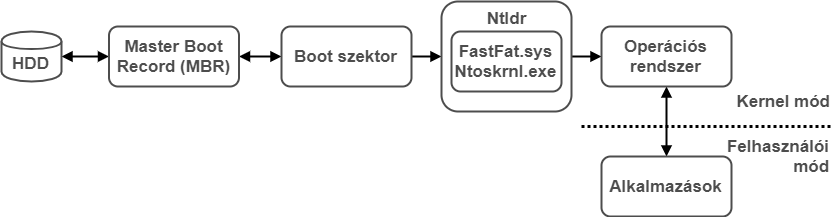
\includegraphics[width=0.9\textwidth]{img/FAT_disk.png}
		\caption{FAT partíció}
        \label{fat_partition}
	\end{figure}

    \noindent Egy partíció formázásakor és a FAT fájlrendszer beállításakor egy úgynevezett Master Boot Record (MBR) jön létre a háttértárolón.\\

    \noindent A Master Boot Record, vagy más néven a partíciós szektor a merevlemez legelső szektorának (azaz az első lemezfelület első sávja első szektorának) elnevezése. \\

    \noindent Csak a particionált merevlemezeknek van Master Boot Recordjuk. \\

    \noindent A Master Boot Record a merevlemez legelején, az első partíció előtt található meg.\\

    \noindent A Master Boot Record egy kisebb végrehajtható kódot, amit Master Boot Code-nak hívunk, és egy partíciós táblát tartalmaz. \\

    \noindent Egy új partíció becsatolásakor a Master Boot Record végrehajtja a Master Boot Code-ot, és átadja a vezérlést a lemez boot szektorának.\\

    \renewcommand{\arraystretch}{2}
    {\footnotesize
      \begin{tabular}{|p{6cm}|p{8cm}|} \hline
      Hard disk & Háttértároló, ami egy vagy két partíciót tartalmaz. \\ \hline
      Boot szektor & Összesen: Bootolható partíció, amely információkat tartalmaz a lemez kialakításáról, a fájlrendszer struktúrájáról. Itt tárolódik a boot code is, amely az Ntdlr-t tölti be. \\ \hline
      Master Boot Record & Olyan végrehajtható kódot tartalmaz, amit a rendszer BIOS (Basic Input/Output System) tölt be a memóriába. A kód a partíciós tábla alapján eldönti, hogy melyik partíció aktív vagy bootolható. \\ \hline
      Ntldlr.dll & A processzort (CPU) védett módba állítja, elindítja a fájlrendszert, majd kiolvassa a Boot.ini fájl tartalmát. Ezek az információk meghatározzák a kezdeti beállításokat és a kezdeti „boot menu” opciókat.

Az Ntldr Windows NT alapú operációs rendszerek betöltőprogramja, amelynek feladata az alapvető hardverkonfigurációs jellemzők felderítése és az ezeknek megfelelő rendszermagváltozat betöltése és elindítása. \\ \hline
      Fastfat.sys & System file driver a FAT 16-hoz és a FAT 32-höz.  \\ \hline
      Ntoskrnl.exe & Információt ad arról, hogy melyik system device drivert kell betölteni, és hogy mi a megfelelő betöltési sorrend. \\ \hline
      Kernel mód & Az a végrehajtó mód, amely lehetőséget biztosít a kódoknak, hogy közvetlen hozzáférjenek az összes hardverhez és a memóriához a rendszerben. \\ \hline
      Felhasználói mód & Az a végrehajtó mód, ahol az alkalmazások futnak. \\ \hline
      \end{tabular}
    }
    \renewcommand{\arraystretch}{1}\\

    \paragraph*{A FAT fájlrendszer fizikai szerkezete, lemezkezelése}

    \noindent A klaszter a legkisebb egység a lemezen, amit le lehet foglalni egy fájl tárolásához. A szektor a tárolás egysége a háttértárolón. Ha például egy háttértároló 512 bájtos szektorméretet használ, akkor az 512 bájtos klaszter egy szektort, míg a 4 kilobájtos klaszter nyolc szektort foglal magában.\\

    \noindent A klaszterek a partíció kezdetétől sorban vannak megszámozva. Mivel a FAT fájlrendszer adatklaszterei a BIOS Parameter Block, a fenntartott szektorok és két FAT struktúra után találhatók, így a FAT formázás nem garantálja, hogy az adatklaszterek illeszkednek a klaszterhatárokra.\\

    \noindent Mivel a FAT 16 és a FAT 32 különböző méretű klaszterekkel dolgozik, a kötet méretétől függően, így az összes fájlrendszernek megvan a maximálisan támogatott klaszterszáma. Minél kisebb a klaszter mérete, annál hatékonyabb az adattárolás a lemezen.\\

    \noindent A nevekben elhelyezkedő számok utalnak arra, hogy hány bit szükséges a FAT tábla egy bejegyzésének tárolására:
    \begin{itemize}[topsep=8pt,itemsep=4pt,partopsep=4pt, parsep=4pt]
        \item FAT16:
        \begin{itemize}
            \item 16 bites bejegyzések
            \item (Ez 216 klasztert jelent.)
        \end{itemize}
        \item FAT32:
        \begin{itemize}
            \item 32 bites bejegyzések, amiből 4 bit a FAT bejegyzésre van félretéve.
            \item (Tehát maximum 228 klaszter lehetséges.)\\
        \end{itemize}
    \end{itemize}

    \noindent A \textbf{FAT16} fájlrendszer méretkorlátai\\

    \noindent \renewcommand{\arraystretch}{2}
    {\footnotesize
      \begin{tabular}{|p{6cm}|p{9cm}|} \hline
      Leírás & Maximális fájlméret \\ \hline \hline
      Maximális fájlméret & Összesen: 4 GB - 1 bájt (azaz 232 bájt - 1 bájt). \\ \hline
      Maximális kötetméret & Összesen: 4 GB. \\ \hline
      Fájlok maximális száma kötetenként & Megközelítően 65 536 (azaz 216 darab fájl). \\ \hline
      Maximum hány fájl vagy könyvtár lehet a gyökérkönyvtárban? & 512 db \\ \hline
      \end{tabular}\\
    }
    \renewcommand{\arraystretch}{1}\\

    \noindent A \textbf{FAT32} fájlrendszer méretkorlátai\\

    \noindent \renewcommand{\arraystretch}{2}
    {\footnotesize
      \begin{tabular}{|p{6cm}|p{9cm}|} \hline
      Leírás & Maximális fájlméret \\ \hline \hline
      Maximális fájlméret & Összesen: 4 GB - 1 bájt (azaz 232 bájt - 1 bájt). \\ \hline
      Maximális kötetméret & 32 GB (implementációfüggő). \\ \hline
      Fájlok maximális száma kötetenként & 4 194 304 darab. \\ \hline
      Maximum hány fájl vagy könyvtár lehet a gyökérkönyvtárban? & 65 536 db \\ \hline
      \end{tabular}
    }
    \renewcommand{\arraystretch}{1}\\

    \paragraph*{A FAT fájlrendszer kötetszervezése, felépítése}

        {\footnotesize
    \begin{centering}
        \noindent \renewcommand{\arraystretch}{2}
            \begin{tabular}{|c|c|c|c|c|c|} \hline
                \textbf{Boot sector} & \makecell{Reserved \\ sectors} & \textbf{FAT} (1) & \makecell{\textbf{FAT (2)}\\Copy of FAT (1)} & \textbf{Root folder} & \textbf{Files and folders} \\ \hline
            \end{tabular}
        \renewcommand{\arraystretch}{1}\\
    \end{centering}
        }

    \renewcommand{\arraystretch}{2}
    {\footnotesize
      \begin{tabular}{|p{6cm}|p{9cm}|}
      \hline
        Elemek & Leírás \\ \hline \hline
        Boot sector & Bootolható partíció, amely információkat tartalmaz a lemez kialakításáról, a fájlrendszer struktúrájáról. Itt tárolódik a boot code is. \\ \hline
        Reserved sectors & A szektorok száma, ami megelőzi az első FAT köteget, és tartalmazza a boot szektort. \\ \hline
        FAT 1 & Eredeti FAT kötet. \\ \hline
        FAT 2 & Biztonsági mentés a FAT kötetről. \\ \hline
        Root folder & Leírja a fájlokat és a mappákat, amelyek a partíció gyökerében találhatóak. \\ \hline
        Files and folders & A fájlok és mappák adatait tartalmazza, amelyek a fájlrendszerben találhatóak. \\ \hline
      \end{tabular}
  }
  \renewcommand{\arraystretch}{1}\\\\

    \noindent A FAT fájlrendszer az elnevezését a benne megvalósított fájlláncolási eljárásról kapta. Ebben a fájlláncolási eljárásban nemes egyszerűséggel felvettek egy táblázatot, ami megmondja, hogy az n.-ik klaszteren elhelyezkedő fájl következő darabja pontosan hol található. A FAT táblában szerepelhet a valós értékek mellett egy-két extrém érték is, amelyek a fájl végét, hibás klasztert vagy üres blokkot jelölhetnek.\\

    \noindent A FAT tábla összesen két példányban került a lemezre, így ha az egyik megsérült valamilyen oknál fogva, akkor az a másikból helyreállítható volt. Sajnálatos módon a tervezésnél a két FAT tábla (az eredeti és a duplikátum) pontosan egymás mögött helyezkedik el, így egy szerencsétlen hardverhiba esetén mind a kettő akár egyszerre is megsérülhet. A dupla hibalehetőségre viszont az informatikában nem lehet tervezni, mivel elég költséges.\\

    \noindent A FAT fájlrendszeren egy fájl neve nyolc (8) ASCII karakter lehetett, amelyet egy háromkarakteres (3) kiterjesztés követett. Az MS-DOS és a Microsoft Windows operációs rendszerek a kiterjesztés alapján döntötték el (és ez alapján döntik el a mai napig is) egy fájl típusát.\\

    \noindent A könyvtárak és a kötetazonosítók attribútumokkal voltak jelölve. A FAT fájlrendszer egyéb attribútumai (mint például a rendszerattribútum, a rejtett attribútum, az archív attribútum és a csak olvasható attribútum) eléggé „gyengére” sikerültek, mivel alkalmazásfüggő volt, hogy a fájlrendszer figyelembe vette-e őket, vagy sem. A FAT fájlrendszer eredetileg csak az utolsó módosítás dátumát tárolta, azt is csak két másodperces felbontással.\\

    \noindent A Microsoft Windows 95 operációs rendszerben bevezették az úgynevezett LFN-t, azaz a hosszú fájlnév támogatást.\\

    \noindent Minden egyes könyvtárbejegyzés tárolja a fájl első darabjának helyét (a kezdő klasztert), és a FAT fájlrendszerben a fájl végigolvasásához innen indulva kell végigjárni a FAT táblát.

    \paragraph*{A fragmentáció a FAT fájlrendszerekben}

    \noindent A FAT fájlrendszernek sosem voltak különféle mechanizmusai, eljárásai a fájlok töredezettségének a megakadályozására, illetve kezelésére. A fájltöredezettség azt jelenti, hogy a fájl egyes darabkái egymástól messze található klaszterekbe kerülnek (ez az úgynevezett first-fit allokációs módszer). Így a fájlok beolvasásakor a merevlemez olvasófejének rendkívül sokat kell ide-oda mozognia, ezáltal nagyon lassú lett a fájlok beolvasása, a merevlemez pedig folyamatosan „berregett”.\\

    \noindent A FAT fájlrendszerhez mellékeltek emiatt egy úgynevezett defragmentáló (töredezettségmentesítő) programot, amellyel „on-demand”, azaz azonnal sorba lehetett rendezni a fájlrendszeren található állományokat. Így könnyen megtörténhetett az, hogy egy akkoriban lassan bootoló 486-os számítógép szinte „szárnyakat kapott” egy egyszerű defragmentálástól.\\

    \noindent A defragmentálás mindenesetre akkoriban egy rendkívül időigényes és veszélyes folyamat volt. A veszélyesség abban az értelemben nyilvánult meg, hogy egy pillanatnyi áramszünet komoly adatvesztéses károkat okozhatott a fájlrendszerben.\\

    \paragraph*{A FAT fájlrendszer napjainkban}

    \noindent A FAT fájlrendszer az MS-DOS, a Microsoft Windows 95 és a Microsoft Windows 98 operációs rendszerek natív fájlrendszere. Manapság az MP3 és az MP4 lejátszókon, a flash-drive-okon, a memóriakártyákon és a digitális kamerákon is használnak FAT fájlrendszert, mert kompatibilis szinte minden operációs rendszerrel.\\

    \noindent A FAT eredeti változatai a nagyobb meghajtók esetében a rendelkezésre álló helyet nagyon rosszul kezelték, éppen ezért hozta létre a Microsoft a FAT fájlrendszer bővített 32-bites változatát, amit FAT 32-nek neveztek el. Az „eredeti merevlemezes” FAT változatra FAT 16-osként szokás hivatkozni, mert az allokációs egységek számát 16 biten tárolja. A FAT fájlrendszernek ezen a két változatán kívül (FAT16, FAT32) létezett még 12 bites változata is, amit FAT 12-nek nevezünk. Utóbbi azonban kizárólag hajlékonylemezes egységeken volt használatban.\\

    \noindent A FAT fájlrendszer napjainkban elavult fájlrendszernek tekinthető, mert sem naplózási, sem biztonsági jogosultságok tárolására nem alkalmas.\\

	\paragraph*{NTFS}

    \noindent Az NTFS fájlrendszer (avagy New Technology File System, magyarul az új technológiájú fájlrendszer) a Microsoft korábbi FAT fájlrendszerét váltotta le.\\

    \noindent A Microsoft Windows NT operációs rendszerben jelent meg először az NTFS fájlrendszer.\\

    \noindent Manapság széles körben elterjedt az NTFS fájlrendszer, ugyanis rengeteg újítás, újdonság és extra funkció érhető el benne, ami az elavult FAT fájlrendszerben nem volt elérhető, és emiatt a FAT fájlrendszer hiányosságaként soroltuk fel az előző pontban. Ilyenek például
    \begin{itemize}[topsep=8pt,itemsep=4pt,partopsep=4pt, parsep=4pt]
        \item metaadatok támogatása,
        \item fejlettebb adatstruktúrák támogatása,
        \item sebesség és a megbízhatóság növekedése,
        \item lemezterület optimálisabb felhasználás,
        \item rendelkezik hozzáférés-védelmi listával
        \item naplózás
    \end{itemize}

    \noindent Elterjedése a Microsoft operációs rendszereken kívül akadályozott, mivel az NTFS fájlrendszer pontos speciikációja a Microsoft szabadalma.\\

    \noindent Az NTFS fájlrendszer 64 bites indexeket használ a klaszterek kiválasztásához, így nem pazarol az amúgy is szűkös hellyel. A 64 bites indexelési módszernek köszönhetően az NTFS fájlrendszernek az elvileg elérhető maximális partíciómérete 16 exabájt (16 EB), ám a gyakorlatban 2 terabájtnál (2 TB) nagyobb partíciókat már nem kezel.\\

    \noindent Az NTFS fájlrendszer teljesen a Microsoft Windows NT operációs rendszer biztonsági modelljére épül. Pontosabban a DACL (Discretionary Access Control List) és SACL (System Access Control List, magyarul hozzáférési listák) biztonsági megfontolásaira épül, így az NTFS fájlrendszeren belül megadható, hogy melyik felhasználó mikor és mit végezhet egy-egy fájllal, továbbá minden elvégzett művelet visszakövethető benne. Ez a biztonsági modell az, amivel az NTFS fájlrendszer valóban hatalmas előrelépés volt a FAT fájlrendszerhez képest. Az NTFS fájlrendszer mellett szól még az is, hogy egy többfelhasználós környezetben, mint amilyen a Microsoft Windows NT operációs rendszer szerver verziója, feltétlenül szükséges egy ilyenfajta biztonsági modell követése.\\

    \noindent A FAT fájlrendszerrel ellentétben az NTFS fájlrendszer volt az első olyan Microsoft Windows platformú fájlrendszer, ami natívan (bármiféle „hack” nélkül) támogatta a hosszú fájlneveket.\\

    \noindent A FAT fájlrendszer legnagyobb hibáját, miszerint a FAT fájlrendszerben nincs semmilyen hibatűrő\footnote{A hibatűrő megoldás alatt azt értjük, hogy ha a nyitott fájlok módosítása, szerkesztése során fellép egy esetleges rendszerhiba, például a számítógép „lefagy”, akkor a fájlrendszer -partíción tárolt adatok nem vállnak inkonzisztenssé.} megoldás, az NTFS fájlrendszer ügyesen megoldotta.\\

    \noindent Az NTFS fájlrendszer megoldása az lett, hogy vezet egy beépített fájlművelet-végzési nyilvántartást (azaz egy úgynevezett log fájlt). Ebbe a speciális log fájlba minden egyes fájlművelet során egy bejegyzést tesz. Így amikor egy esetleges rendszerhiba következik be (pl. a fentebb említett „lefagyás”), akkor az újrabootolás során a log fájlok alapján azonnal meg lehet állapítani, hogy a rendszerhiba bekövetkezésekor történt-e bármiféle adatvesztés, vagy sem. Amennyiben a log fájlok alapján megállapítható az adatvesztés megtörténte (a log fájlban benne lesz, hogy a fájlmódosító művelet félbemaradt), akkor el kell indítani az úgynevezett CHKDSK (lemezellenőrző) programot. A CHKDSK program a log fájlt felhasználva megpróbálja visszaállítani az eredeti konzisztens állapotot. A log fájl minden bejegyzése két típusú lehet: vagy ismétlő (redo), vagy visszavonó (undo) parancsot tartalmazhat.\\

    \noindent A log fájl mérete a merevlemeztől függően két és négy megabájt között (2 MB – 4 MB) mozoghat. Ha az NTFS fájlrendszer nem vizsgálná meg mindig, hogy az ismétlő (redo) és a visszavonó (undo) információk szükségesek-e hibajavítás esetére, akkor a log fájl mérete gyorsan megnőne, és így hamar be is telne. Ennek az elkerülése végett az összes módosított adatot lemezre menti az NTFS fájlrendszer, és törli a log fájl tartalmát. Ez a vizsgálat az úgynevezett checkpoint- (határpont-) képzés. A vizsgálat körülbelül minden 4. vagy 5. másodpercben megtörténik.

    \paragraph*{Az NTFS fájlrendszer maximális fájlmérete}

    \renewcommand{\arraystretch}{2}
    {\footnotesize
      \begin{tabular}{|p{6cm}|p{9cm}|}
      \hline
        \textbf{Elemek} & \textbf{Határ} \\ \hline \hline
        Maximális fájlméret & Elvi megvalósíthatóság: 16 exabájt – 1 kB (264 bájt – 1 kB)
        Megvalósított: 16 terabájt – 64 kB (244 bájt – 64 kB)  \\ \hline
        Maximális kötetméret & Elvi megvalósíthatóság: 264 klaszter – 1 klaszter
        Megvalósított: 256 terabájt – 64 kB (azaz 232 klaszter – 1 klaszter)  \\ \hline
        Fájlok maximális száma kötetenként & 4 294 967 295 (azaz 232 – 1 fájl)  \\ \hline
      \end{tabular}
  }
  \renewcommand{\arraystretch}{1}\\

    \paragraph*{Az NTFS fájlrendszer maximális kötetmérete}

    \noindent Elméletben a maximális NTFS kötetméret 264 - 1 klaszter (foglalási egység). Ennek ellenére a maximális NTFS kötetméret a Windows XP Professional megvalósításának megfelelően 232 - 1 klaszter.\\

    \noindent \renewcommand{\arraystretch}{2}
    {\footnotesize
      \begin{tabular}{|p{6cm}|p{9cm}|}
      \hline
        \textbf{Partíció méret} & \textbf{NTFS klaszterméret} \\ \hline \hline
        7 megabájt (MB) – 512 megabájt (MB) & 512 bájt (B)  \\ \hline
        513 megabájt (MB) – 1,024 megabájt (MB) & 1 kilobájt (kB)  \\ \hline
        1,025 megabájt (MB) – 2 gigabájt (GB) & 2 kilobájt (kB) \\ \hline
        2 gigabájt (GB) – 2 terabájt (TB) & 4 kilobájt (kB) \\ \hline
      \end{tabular}
  }
  \renewcommand{\arraystretch}{1}\\

    \paragraph*{Az NTFS fájlrendszer kötetszervezése, felépítése}

    \begin{centering}
        \renewcommand{\arraystretch}{2}
        {\footnotesize
          \begin{tabular}{|c|c|c|c|} \hline
          \textbf{NTFS Boot sector} & \makecell{\textbf{MFT} \\ Master File Table} & \textbf{File System Data} & \textbf{Copy of MFT} \\ \hline
      \end{tabular}
  }
  \renewcommand{\arraystretch}{1}\\
    \end{centering}

    \noindent \renewcommand{\arraystretch}{2}
    {\footnotesize
      \begin{tabular}{|p{6cm}|p{9cm}|}
      \hline
        \textbf{Elemek} & \textbf{Leírás} \\ \hline \hline
        NTFS Boot Sector & Tartalmazza a BIOS paraméterblokkot, ami információkat tárol a lemez kialakításáról és a fájlrendszer struktúrájáról; a „boot code” is itt tárolódik. \\ \hline
        MFT Master File Table & A fájlok eléréséhez szükséges információkat tartalmazza, amelyek az NTFS fájlrendszerű partíción találhatók. \\ \hline
        File System Data & Minden más olyan adatot tárol, amelyeket a Master File Table már nem. \\ \hline
        Master File Table Copy & Biztonsági mentés a Master File Table-ről, ha az eredetin tárolt adatokhoz nem lehet hozzáférni. \\ \hline
      \end{tabular}
  }
  \renewcommand{\arraystretch}{1}\\

    \paragraph*{Az NTFS fájlrendszer fizikai szerkezete, lemezkezelése}

    \noindent Az NTFS fájlrendszer a fájlok és a könyvtárak adatai mellett egy sereg egyéb fájlt is használ a lemezkezeléssel összefüggő adatok tárolása végett. Ezekben a fájlokban és más, az NTFS fájlrendszerrel kapcsolatos fájlban, illetve könyvtárban tárolt adatok összességét úgynevezett metaadatnak (metadata) nevezzük. Egy NTFS fájlrendszerbeli partíció formázása során 11 metaadatfájl jön létre. A metaadatfájlok nem láthatóak egyszerűen semmilyen felsorolásban, viszont ha tudjuk, mi az általunk keresett a metaadatfájl neve, akkor kilistáztathatjuk.\\

    \noindent Az NTFS fájlrendszer legfeljebb 32 000 Unicode karakter hosszúságú elérési útvonalakat támogat, amelyeknek minden komponense (ami egy könyvtár vagy egy fájlnév) legfeljebb 255 Unicode karakter hosszúságú lehet. Bizonyos azonosító neveket a rendszer azonban fenntart a saját használatra. Ennek az az oka, hogy az NTFS fájlrendszer metaadatai szabályos (ámbár rejtett és általában nem hozzáférhető) fájlokban tárolódnak; emiatt a felhasználói adatállományok nem használhatják fel a neveiket. Ezek a rendszerfájlok mindig az NTFS fájlrendszerű kötet gyökerében tárolódnak, és kizárólag a gyökérkönyvtárban vannak fenntartva.\\

	\subsection*{Ext fájlrendszer}

    \noindent Az „ext” kifejezés a fájlrendszerek neveiben az extended (magyarul kiterjesztett) kifejezést takarja. \\

    \noindent Az extended fájlrendszer volt az első kifejezetten a UNIX-szerű GNU/LINUX operációs rendszerekhez készített fájlrendszer, amely örökölte az UFS (UNIX File System) fájlrendszer metaadat-szerkezetét, és arra készült, hogy a Minix operációs rendszer fájlrendszerének a hibáit kiküszöbölje.\\

    \noindent A hibák kiküszöbölése többek között a Minix operációs rendszer fájlrendszer-határainak kiterjesztése, például:
    \begin{itemize}
        \item a maximális méret, amely a 16 bites offszet miatt csak maximálisan 64 megabájt (64 MB) lehetett, illetve
        \item a maximális fájlnévhosszúság, amely csak 14 karakter lehetett.
    \end{itemize}
    Ennek megoldásához egy virtuális fájlrendszerréteget tettek a Linux-kernelbe\footnote{Az operációs rendszer magja. Ez a rész tartalmazza a hardver eszközöket kezelő programot is.}, mellyel a maximális méret két gigabájtra (2 GB), a fájlnevek hosszúsága pedig 255 karakteresre növekedhetett.\\

    \noindent Hiányossága volt azonban az, hogy mindezek ellenére nem biztosította a fájlok egyenkénti elérését, és nem rögzítette a fájlok módosításának idejét!

    \subsection*{Ext2 fájlrendszer}

    \noindent Az extended fájlrendszer következő verziója az „ext2” fájlrendszer lett (second extended filesystem – második kiterjesztett fájlrendszer).\\

    \noindent Az ext2 fájlrendszer, amely a GNU/LINUX operációs rendszereken kívül más rendszereken is megjelent, több Linux disztribúció alapértelmezett fájlrendszere volt, amíg az utódja, az „ext3” fájlrendszer  el nem készült.\\

    \noindent Az ext2 fájlrendszer nagy előnye a többi más fájlrendszerekhez képest, hogy már a tervezésénél készültek a folytatására, továbbfejlesztésére úgy, hogy a még meg nem valósított, azaz nem implementált funkcióknak meghagyták benne a helyet.

    \paragraph*{Az ext2 fájlrendszer adatszerkezete}

    \noindent A szabad területet az ext2 fájlrendszer blokkokra osztja, a blokkokat pedig további csoportokra osztja tovább. \\

    \noindent Egy-egy fájl – amennyire csak lehet – egy csoportba tartozik, hogy a csökkentse a fájlrendszer szabad területének töredezését, és hogy csökkentse a keresést nagyméretű folytonos elérésű fájlok esetén.\\

    \noindent Minden csoport tartalmazza a saját leírótábláját és a szuperblokk leírójának másolatát, egy blokktérképet, amely számon tartja, hogy mely fizikai részek foglaltak, és melyek nem.\\

    \noindent Ezeken kívül tartalmaz még egy úgynevezett \textbf{i-node}-ot\footnote{A UNIX fájlrendszerének megszervezésében használatos, a fájllal kapcsolatos információkat tárolja}, melynek szintén van blokktérképe és leírótáblája. Ezek címeit a csoportleíró tartalmazza.

    \paragraph*{Az i-node-ok használata az ext2 fájlrendszerben}

    Minden egyes fájlt és könyvtárat egy-egy i-node ír le (\ref{ref:ex2inode}. ábra).\\
    Ez tartalmazza a fájlok tulajdonságait:
    \begin{itemize}[topsep=8pt,itemsep=4pt,partopsep=4pt, parsep=4pt]
        \item hozzáférési jogok,
        \item engedélyek,
        \item fájlméret és
        \item a fájl helye a merevlemezen
    \end{itemize}

    \noindent Az i-node struktúra 15 mutatót tartalmaz, melyből 12 fix, és a 13-astól kezdve pedig újabb i-node-okra mutathat, amennyiben a fájl nem fér bele egy i-node-ba.

	\begin{figure}[H]
		\centering
		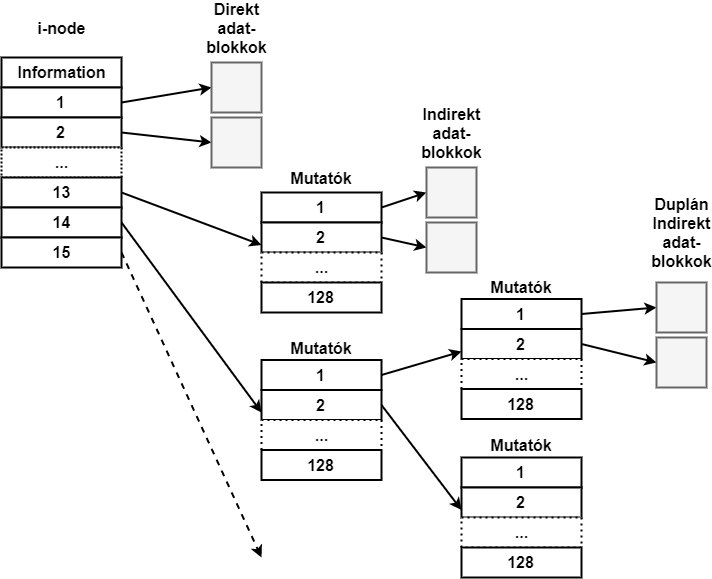
\includegraphics[width=0.8\textwidth]{img/ext2inode.png}
		\caption{i-node szerkezete}
        \label{ref:ex2inode}
	\end{figure}

    \paragraph*{A könyvtárak az ext2 fájlrendszerben}

    Minden egyes könyvtár további könyvtárbejegyzéseket tartalmazhat. Ezek a bejegyzések azonosítják az egyes fájlokat az egyes i-node-okhoz.
    Tartalmazhatják az
    \begin{itemize}[topsep=8pt,itemsep=4pt,partopsep=4pt, parsep=4pt]
        \item i-node számát,
        \item a fájlnév hosszúságát és
        \item a fájl nevét.
    \end{itemize}

    \noindent Egy megadott keresés során a kereső ezeken az adatokon megy végig, ezeket az adatokat vizsgálja meg. A gyökérkönyvtár mindig az i-node második eleme, így a rendszer a felcsatlakoztatás (mount) során rögtön megtalálja. Az alkönyvtárak a fájlokhoz hasonlóan szerepelhetnek a táblában, egy saját i-node számmal és egy saját névvel. A hivatkozások pedig ugyancsak egy i-node azonosítóhoz rendelnek több nevet, így végül mindegyik hivatkozás ugyanarra a fizikai helyre mutat.\\

    \noindent Az aktuális munkakönyvtár [. (a pont)] és a szülő munkakönyvtár [.. (a dupla pont)] ugyanígy tárolódik a fájlrendszeren belül, vagyis minden egyes könyvtár tartalmazza a saját és a szülőjének a nevét és az ő azonosítóját. Ezek a könyvtárak létrehozásakor automatikusan létrejönnek, és csak a könyvtárral együtt törölhetők!

    \paragraph*{Az ext2 fájlrendszer határai}

    \noindent A fájl méretének és a meghajtó méretének határait a blokkok mérete határozza meg az ext2 fájlrendszerben, amelyet az adott architektúra lapmérete határoz meg a legfőképpen. Ezek a határok a fájlrendszer felépítése során rögzülnek, és még számos felhasználói programnak is lehetnek határai [például a két gigabájtnál (2GB) nagyobb fájlok esetében].\\

    \noindent Az ext2 fájlrendszer maga nem tartalmazza a lehetőséget az adatok tömörített tárolására.

    \subsection*{Ext3 fájlrendszer}

    \noindent Az ext3 fájlrendszer (third extended filesystem – harmadik kiterjesztett fájlrendszer) az ext2 fájlrendszer utódja.

    \begin{itemize}[topsep=8pt,itemsep=4pt,partopsep=4pt, parsep=4pt]
        \item Az ext2 fájlrendszerhez képest naplózást is tartalmaz.\\\\
        {\footnotesize \noindent {\color{blue} \faLightbulbO\ $\triangleright$ } }
        {\footnotesize
        A naplózás elsősorban a biztonságot növeli, és lehetővé teszi azt, hogy szabálytalan leállás bekövetkezése után ne kelljen az egész fájlrendszert újra ellenőrizni.
        $\triangleleft$ \faLightbulbO}
        \item Visszafelé irányú kompatibilitása lehetővé teszi, hogy bármiféle adatmentés nélkül átalakítható legyen az ext2 fájlrendszerből.
        \item Tesztek azt mutatják, hogy a hasonló fájlrendszerekhez képest kevesebb processzor- (CPU-) erőforrást használ, és egyszerűsége.
        \item A nagy felhasználói bázisa miatt biztonságosabb.
        \item A naplózáson kívül az ext3 fájlrendszer lehetővé tette a kikapcsolás nélküli növelés és a sok fájlt tartalmazó könyvtárak H-fával való indexelését.
        \item Az ext2 fájlrendszerre írt diagnosztikai és javító eszközök kisebb módosítással használhatók az ext3 fájlrendszerrel.
    \end{itemize}

    \noindent Ezek nélkül az ext3 fájlrendszer teljesen azonos lett volna az ext2 fájlrendszerrel.\\

    {\footnotesize \noindent {\color{blue} \faLightbulbO\ $\triangleright$ } }
    {\footnotesize
    \noindent \textbf{Az ext3 fájlrendszer háromszintű naplózása}

    \begin{enumerate}[topsep=8pt,itemsep=4pt,partopsep=4pt, parsep=4pt]
        \item Ezen a naplózási szinten a metaadat és a fájl is egy az egyben a naplóba íródik. Abban az esetben, ha folyamatosan nagy fájlokkal dolgozunk, akkor ez a fajta naplózás gyorsíthat is, de alapvetően inkább lassít a dupla írás miatt.

        \item Ezen a naplózási szinten egy rendezett naplózás található, azaz csak a metaadat. íródik a naplóba, de garantált az, hogy az aktuális metaadat. csak akkor kerül elfogadásra (commitálásra), ha a teljes fájl már a fizikai helyére került. A legtöbb GNU/LINUX disztribúcióban ezt használják. Tegyük fel, hogy egy fájl kiíródása közben baj történik (áramkimaradás vagy kernelpánik). Ekkor a napló jelzi, hogy a fájl írása nem fejeződött be, ezért következő indításkor a módosítások megsemmisülnek. A módosított fájlokban azonban így könnyen sérülések keletkezhetnek, ugyanis a fájl eredeti változata nem tárolódik, ezáltal sem az eredeti, sem az új verzió nem állítható vissza.

        \item Ezen a naplózási szinten egy visszaírás található, azaz csak a metaadat. íródik ki a naplóba, de a naplóba írás a tényleges írás előtt és után is egyaránt megtörténhet. Ebben az esetben egy hirtelen leálláskor az írás alatt lévő fájlok könnyebben sérülhetnek. Például egy hozzáfűzés megszakadásakor a fájl nagyobb, mint ahogy az a naplóban található, ellenben ez a fajta aszinkron működés gyakran gyorsabbá teszi a fájlrendszert.
    \end{enumerate}
    $\triangleleft$ \faLightbulbO}\\

    \noindent \textbf{Az ext3 fájlrendszer hátrányai\\}

    \begin{itemize}[topsep=8pt,itemsep=4pt,partopsep=4pt, parsep=4pt]
        \item Az ext2 fájlrendszerrel való visszafelé kompatibilitás miatt számos modern fájlrendszerre jellemző tulajdonság kimaradt az ext3 fájlrendszerből.\\\\
        {\footnotesize \noindent {\color{blue} \faLightbulbO\ $\triangleright$ } }
        {\footnotesize
        A könyvtárankénti fájlok száma is összesen 31 998 darab fájlra korlátozódik az i-node mutatók maximális számából adódóan.}
        \item Az ext3 fájlrendszer nem ellenőrizhető addig, amíg az csatlakoztatva van az operációs rendszerhez.\\\\
        {\footnotesize \noindent {\color{blue} \faLightbulbO\ $\triangleright$ } }
        {\footnotesize
        Az ext3 fájlrendszer fájlrendszer szintjén töredezettségmentesítés sem végezhető el addig, amíg az csatlakoztatva van az operációs rendszerhez, tehát felcsatolt állapotban van. Ellenben a felhasználói szinten vannak erre megfelelő eszközök, amelyek a legnagyobb folyamatos szabad helyeket keresve, fájlokat ide-oda másolgatva működnek, de ehhez viszonylag nagyméretű szabad hely szükséges. Erre általában viszont nincs is nagy szükség, mert az ext3 fájlrendszer igyekszik az egymás után következő fájlokat eleve egymáshoz a lehető legközelebb másolni.
        $\triangleleft$ \faLightbulbO}\\
        \item Törlésnél a fájlrendszer aktívan távolítja el az i-node -okban tárolt adatokat, főleg biztonsági okokból, ezért nincs sok lehetőség a fájlok helyreállítására.
        \item A tömörítést, mint az ext2 fájlrendszer esetén, csak egy kiegészítő program biztosíthatja.
        \item Nincs támogatás egy aktuális állapotkép készítésére, mely időnként mentené a fájlrendszer állapotát.
        \item Nem számol ellenőrző összegeket a naplóbejegyzésekhez.\\\\
        {\footnotesize \noindent {\color{blue} \faLightbulbO\ $\triangleright$ } }
        {\footnotesize
        Ez akkor jelenthet igazán gondot, ha a merevlemez nem sorrendben írja az adatokat annak érdekében, hogy csökkentse az olvasófej mozgását és ezáltal a meghajtó elhasználódását. Ekkor előfordulhat, hogy egy esetleges leállás pontosan akkor következik be, amikor egy fájlnak az eleje még nem, de egy másik része már a merevlemezre íródott. Ekkor a naplóból való visszaállítás során a kiírt adatok hibás adatokkal íródnak felül, mert a napló nem tudja eldönteni, hogy a fájl melyik része íródott ki.
        $\triangleleft$ \faLightbulbO}\\
    \end{itemize}

	\subsection*{ReiserFS fájlrendszer\\}

    \noindent A ReiserFS fájlrendszer lehetővé teszi egy blokkos eszközön (block device) változó méretű fájlok tárolását és könyvtárstruktúrába rendezését.\\

    \noindent A ReiserFS fájlrendszer egy olyan fájlrendszer, amely csak és kizárólag a GNU/LINUX operációs rendszer alatt használható jelenleg korlátozás nélkül.\\

    {\footnotesize \noindent {\color{blue} \faLightbulbO\ $\triangleright$ } }
    {\footnotesize
    \noindent A ReiserFS fájlrendszerről a GNU/ Linux operációs rendszer indítása lehetséges, például a GRUB vagy a LILO segítségével (A GRUB képes a ReiserFS fájlrendszert olvasni, a LILO pedig fájlrendszer-független.)

    \noindent A ReiserFS fájlrendszert tartalmazó partíció \emph{\textbf{írására}} nem ismert semmilyen szoftver Microsoft Windows és Mac OS operációs rendszerek alatt.\\

    \noindent Mac OS X operációs rendszer alatt a virtualizáción kívül nincs ismert megoldás a ReiserFS fájlrendszer írására és olvasására.\\

    \noindent A Microsoft Windows operációs rendszerek alatt olvashatjuk a ReiserFS fájlrendszert a megfelelő third-party alkalmazás (például: RFSTool) segítségével.
    $\triangleleft$ \faLightbulbO}

    \paragraph*{A ReiserFS előnyei\\}

    \begin{itemize}[topsep=8pt,itemsep=4pt,partopsep=4pt, parsep=4pt]
        \item Jobb lemezterület-kihasználás.\\

        {\footnotesize \noindent {\color{blue} \faLightbulbO\ $\triangleright$ } }
        {\footnotesize
        \noindent A ReiserFS fájlrendszerben az összes adat kiegyensúlyozott B*-fastruktúrába van szervezve. A fastruktúra jobban ki tudja használni a lemezterületet, mivel a kis fájlok közvetlenül a B*-fa levélcsomópontjaiban kerülnek tárolásra, nem pedig egy másik helyen és csak egy mutató mutat a tényleges tárolási helyre. Ezen felül a tárterület nem 1 vagy 4 kilobájtos egységekben kerül lefoglalásra, hanem az adatok pontosan a szükséges méretet foglalják el. Másik előnye az inode-ok dinamikus lefoglalása. Így a rendszer rendkívül rugalmas, szemben például az Ext2-vel, ahol az inode-ok sűrűségét a fájlrendszer létrehozásakor kell megadnunk.
        $\triangleleft$ \faLightbulbO}\\

        \item Jobb lemezhozzáférési teljesítmény.

        {\footnotesize \noindent {\color{blue} \faLightbulbO\ $\triangleright$ } }
        {\footnotesize
        \noindent Kis fájlok esetén az adatok és a (inode) információ általában egymás mellett kerül tárolásra. Ez az információ egyetlen lemez I/O-művelettel kiolvasható, azaz csak egy lemezhozzáférés szükséges a kívánt információ lekéréséhez.
        $\triangleleft$ \faLightbulbO}

        \item Gyors visszaállítás rendszerösszeomlás után.

        {\footnotesize \noindent {\color{blue} \faLightbulbO\ $\triangleright$ } }
        {\footnotesize
        \noindent A legutolsó metaadat-módosításokat nyomkövető napló segítségével a fájlrendszer ellenőrzése nagyon nagy fájlrendszerek esetén is csak néhány másodpercet vesz igénybe.
        $\triangleleft$ \faLightbulbO}

        \item Megbízhatóság az adatnaplózás használatával.

        {\footnotesize \noindent {\color{blue} \faLightbulbO\ $\triangleright$ } }
        {\footnotesize
        \noindent A ReiserFS az adatnaplózást és a sorbarendezett adatmódokat is támogatja, hasonló elven, mint ahogy az Ext3-nál. Az alapértelmezett mód a data=ordered, amely az adatok és metaadatok integritását egyaránt biztosítja, de naplózást csak a metaadatokhoz használ.
        $\triangleleft$ \faLightbulbO}\\
    \end{itemize}
	
    \paragraph*{A ReiserFS fájlrendszer jellemzői\\}

    \begin{itemize}[topsep=8pt,itemsep=4pt,partopsep=4pt, parsep=4pt]
        \item A ReiserFS fájlrendszer a metaadatokat, sőt a négy kilobájtnál nem rövidebb fájltartalmak kivételével mindent egyetlen B+ fában tárol.\\

        {\footnotesize \noindent {\color{blue} \faLightbulbO\ $\triangleright$ } }
        {\footnotesize
        Ez teszi lehetővé a korlátlan számú i-node létrehozását és a nagy könyvtárak tartalmának elérését.
        $\triangleleft$ \faLightbulbO}\\

        \item Több fájl utolsó blokkjait egyetlen lemezblokkban is képes tárolni.\\

        {\footnotesize \noindent {\color{blue} \faLightbulbO\ $\triangleright$ } }
        {\footnotesize
        \noindent Tárolás szempontjából a legtöbb fájlrendszer a fájlokat blokkokra osztva tárolja. A tipikus blokkméret az NTFS fájlrendszer esetén a négy kilobájt (4 kB), és ha az utolsó blokk rövidebb, akkor a különbség elpazarlódik. Ezen javít a ReiserFS fájlrendszer, mert több fájl utolsó blokkjait egyetlen lemezblokkban is képes tárolni. Ez különösen előnyös az UNIX operációs rendszerbeli apró fájlok esetén, például egy /etc könyvtárban. A technológia neve: tail packing.
        $\triangleleft$ \faLightbulbO}\\

        \item A ReiserFS fájlrendszer – a többi UNIX fájlrendszerhez hasonlóan – egyszerűen az i-node-okat a könyvtárstruktúrán kívül tárolja.\\

        {\footnotesize \noindent {\color{blue} \faLightbulbO\ $\triangleright$ } }
        {\footnotesize
        Tehát például egy négy kilobájtos (4 kB) fájl beolvasásához tipikusan hétszer kell „seekelni”: háromszor, hogy a B+ fában a fájlnév alapján megtaláljuk az i-node számát, és háromszor azért, hogy a B+ fában az i-node száma alapján megtaláljuk az adatblokk kezdőcímét, és egyszer még, mielőtt beolvassuk az adatblokkot.
        \noindent A további olvasások már gyorsabbak, mert a B+ fa gyökere és gyökérhez közeli csúcsai ekkor már a cache-ben (cache memory, magyarul belső gyorsítótár) vannak.\\
        \noindent Egy 10000 fájlt tartalmazó könyvtárban a könyvtár tartalmának listázásához szintén körülbelül hét „seekelés” kell, így a könyvtár adatblokkja a benne levő fájlok neveit tartalmazza. Az attribútumokat is tartalmazó listázáshoz („ls –l” parancs) viszont fájlonként további három „seekelés” szükséges, hogy fájlnév alapján megtaláljuk az i-node-ot a B+ fában. Így 10000 fájl esetén 30 007 „seekelésre” van szükség.\\
        \noindent A Reiser4 ezzel szemben közel teszi egymáshoz az összetartozó i-node-okat, emiatt jóval kevesebb „seekelés” kell az „ls –l” parancshoz, és ez sokkal gyorsabbá teszi.
        $\triangleleft$ \faLightbulbO}\\

        \item Hiba esetén, ha az lemezellenőrzés a B+ fában hibát érzékel, azt a jelenlegi ReiserFS fájlrendszer implementáció csak a teljes B+ fa újraépítésével tudja javítani.\\

        {\footnotesize \noindent {\color{blue} \faLightbulbO\ $\triangleright$ } }
        {\footnotesize
        \noindent Az újraépítés nemcsak lassú művelet (mert az egész lemez újraolvasását igényli), hanem sajnos ad hoc is, tehát olyan blokkokat is csúcsnak érzékelhet, amelyek nem azok. Ha tehát a faújraépítés egy fájladatblokkot tévesen csúcsnak érzékel, és ezután néhány bájt módosításával „megjavítja”, akkor épp emiatt az újraépítés okoz további adatvesztést. Nemcsak az a néhány bájt vész el, amit módosítottunk, hanem az egész korábbi fájl is. Ez a nagymértékű adatvesztés a fájlrendszer-ellenőrzés hatására más elven működő fájlrendszerekre nem jellemző, ez tehát ReiserFS fájlrendszer egyik hátránya például az ext2 fájlrendszerhez képest.\\
        \noindent Hardverhiba ellen naplózással sajnálatosan nem lehet védekezni, és ha a lemezen egyes blokkok meghibásodnak, akkor inkonzisztenssé válhat az egész fájlrendszer is, melyre az ellenőrzés deríthet csak fényt (vagy nagyon súlyos hiba esetén már nem is lehet csatolni a fájlrendszert).
        $\triangleleft$ \faLightbulbO}\\

    \end{itemize}

    \paragraph*{A ReiserFS fájlrendszer összehasonlítása más fájlrendszerekkel\\}

    \noindent A ReiserFS fájlrendszer előnyei az ext2 és egyéb korábbi fájlrendszerekhez képest:

    \begin{itemize}[topsep=8pt,itemsep=4pt,partopsep=4pt, parsep=4pt]
        \item nagyobb maximális fájlméret és fájlrendszer méret
        \item a fájlrendszer mérete lecsatolás nélkül is növelhető (ezt az ext3 fájlrendszer is tudja)
        \item journaling, azaz naplózás (az ext3 és ext4 fájlrendszerben már van naplózás)
        \item nagy könyvtárak gyorsabb elérése
        \item nem kell az i-node-ok számát létrehozáskor megadni
        \item a négy kilobájtnál kisebb fájlok, fájlblokkok pazarlásmentes tárolása (tail packing)
    \end{itemize}

    \noindent A ReiserFS fájlrendszer hátrányai az ext2 és egyéb korábbi fájlrendszerekhez képest:
    \begin{itemize}[topsep=8pt,itemsep=4pt,partopsep=4pt, parsep=4pt]
        \item globálisan lockolja (zárolja) a Linux-kernelt
        \item hardverhiba esetén nagymértékű adatvesztés történhet
    \end{itemize}

\end{document} 